%  LaTeX support: latex@mdpi.com 
%  For support, please attach all files needed for compiling as well as the log file, and specify your operating system, LaTeX version, and LaTeX editor.

%=================================================================
\documentclass[remotesensing,article,accept,pdftex,moreauthors]{Definitions/mdpi} 

%--------------------
% Class Options:
%--------------------
%----------
% journal
%----------
% Choose between the following MDPI journals:
% acoustics, actuators, addictions, admsci, adolescents, aerobiology, aerospace, agriculture, agriengineering, agrochemicals, agronomy, ai, air, algorithms, allergies, alloys, analytica, analytics, anatomia, animals, antibiotics, antibodies, antioxidants, applbiosci, appliedchem, appliedmath, applmech, applmicrobiol, applnano, applsci, aquacj, architecture, arm, arthropoda, arts, asc, asi, astronomy, atmosphere, atoms, audiolres, automation, axioms, bacteria, batteries, bdcc, behavsci, beverages, biochem, bioengineering, biologics, biology, biomass, biomechanics, biomed, biomedicines, biomedinformatics, biomimetics, biomolecules, biophysica, biosensors, biotech, birds, bloods, blsf, brainsci, breath, buildings, businesses, cancers, carbon, cardiogenetics, catalysts, cells, ceramics, challenges, chemengineering, chemistry, chemosensors, chemproc, children, chips, cimb, civileng, cleantechnol, climate, clinpract, clockssleep, cmd, coasts, coatings, colloids, colorants, commodities, compounds, computation, computers, condensedmatter, conservation, constrmater, cosmetics, covid, crops, cryptography, crystals, csmf, ctn, curroncol, cyber, dairy, data, ddc, dentistry, dermato, dermatopathology, designs, devices, diabetology, diagnostics, dietetics, digital, disabilities, diseases, diversity, dna, drones, dynamics, earth, ebj, ecologies, econometrics, economies, education, ejihpe, electricity, electrochem, electronicmat, electronics, encyclopedia, endocrines, energies, eng, engproc, entomology, entropy, environments, environsciproc, epidemiologia, epigenomes, est, fermentation, fibers, fintech, fire, fishes, fluids, foods, forecasting, forensicsci, forests, foundations, fractalfract, fuels, future, futureinternet, futurepharmacol, futurephys, futuretransp, galaxies, games, gases, gastroent, gastrointestdisord, gels, genealogy, genes, geographies, geohazards, geomatics, geosciences, geotechnics, geriatrics, grasses, gucdd, hazardousmatters, healthcare, hearts, hemato, hematolrep, heritage, higheredu, highthroughput, histories, horticulturae, hospitals, humanities, humans, hydrobiology, hydrogen, hydrology, hygiene, idr, ijerph, ijfs, ijgi, ijms, ijns, ijpb, ijtm, ijtpp, ime, immuno, informatics, information, infrastructures, inorganics, insects, instruments, inventions, iot, j, jal, jcdd, jcm, jcp, jcs, jcto, jdb, jeta, jfb, jfmk, jimaging, jintelligence, jlpea, jmmp, jmp, jmse, jne, jnt, jof, joitmc, jor, journalmedia, jox, jpm, jrfm, jsan, jtaer, jvd, jzbg, kidneydial, kinasesphosphatases, knowledge, land, languages, laws, life, liquids, literature, livers, logics, logistics, lubricants, lymphatics, machines, macromol, magnetism, magnetochemistry, make, marinedrugs, materials, materproc, mathematics, mca, measurements, medicina, medicines, medsci, membranes, merits, metabolites, metals, meteorology, methane, metrology, micro, microarrays, microbiolres, micromachines, microorganisms, microplastics, minerals, mining, modelling, molbank, molecules, mps, msf, mti, muscles, nanoenergyadv, nanomanufacturing,\gdef\@continuouspages{yes}} nanomaterials, ncrna, ndt, network, neuroglia, neurolint, neurosci, nitrogen, notspecified, %%nri, nursrep, nutraceuticals, nutrients, obesities, oceans, ohbm, onco, %oncopathology, optics, oral, organics, organoids, osteology, oxygen, parasites, parasitologia, particles, pathogens, pathophysiology, pediatrrep, pharmaceuticals, pharmaceutics, pharmacoepidemiology,\gdef\@ISSN{2813-0618}\gdef\@continuous pharmacy, philosophies, photochem, photonics, phycology, physchem, physics, physiologia, plants, plasma, platforms, pollutants, polymers, polysaccharides, poultry, powders, preprints, proceedings, processes, prosthesis, proteomes, psf, psych, psychiatryint, psychoactives, publications, quantumrep, quaternary, qubs, radiation, reactions, receptors, recycling, regeneration, religions, remotesensing, reports, reprodmed, resources, rheumato, risks, robotics, ruminants, safety, sci, scipharm, sclerosis, seeds, sensors, separations, sexes, signals, sinusitis, skins, smartcities, sna, societies, socsci, software, soilsystems, solar, solids, spectroscj, sports, standards, stats, std, stresses, surfaces, surgeries, suschem, sustainability, symmetry, synbio, systems, targets, taxonomy, technologies, telecom, test, textiles, thalassrep, thermo, tomography, tourismhosp, toxics, toxins, transplantology, transportation, traumacare, traumas, tropicalmed, universe, urbansci, uro, vaccines, vehicles, venereology, vetsci, vibration, virtualworlds, viruses, vision, waste, water, wem, wevj, wind, women, world, youth, zoonoticdis 
% For posting an early version of this manuscript as a preprint, you may use "preprints" as the journal. Changing "submit" to "accept" before posting will remove line numbers.

%---------
% article
%---------
% The default type of manuscript is "article", but can be replaced by: 
% abstract, addendum, article, book, bookreview, briefreport, casereport, comment, commentary, communication, conferenceproceedings, correction, conferencereport, entry, expressionofconcern, extendedabstract, datadescriptor, editorial, essay, erratum, hypothesis, interestingimage, obituary, opinion, projectreport, reply, retraction, review, perspective, protocol, shortnote, studyprotocol, systematicreview, supfile, technicalnote, viewpoint, guidelines, registeredreport, tutorial
% supfile = supplementary materials

%----------
% submit
%----------
% The class option "submit" will be changed to "accept" by the Editorial Office when the paper is accepted. This will only make changes to the frontpage (e.g., the logo of the journal will get visible), the headings, and the copyright information. Also, line numbering will be removed. Journal info and pagination for accepted papers will also be assigned by the Editorial Office.

%------------------
% moreauthors
%------------------
% If there is only one author the class option oneauthor should be used. Otherwise use the class option moreauthors.

%---------
% pdftex
%---------
% The option pdftex is for use with pdfLaTeX. Remove "pdftex" for (1) compiling with LaTeX & dvi2pdf (if eps figures are used) or for (2) compiling with XeLaTeX.

%=================================================================
% MDPI internal commands - do not modify
\firstpage{1} 
\makeatletter 
\setcounter{page}{\@firstpage} 
\makeatother
\pubvolume{1}
\issuenum{1}
\articlenumber{0}
\pubyear{2024}
\copyrightyear{2024}
\externaleditor{Academic Editor: }
\datereceived{29 January 2024} 
\daterevised{5 March 2024} % Comment out if no revised date
\dateaccepted{8 March 2024} 
\datepublished{ } 
%\datecorrected{} % For corrected papers: "Corrected: XXX" date in the original paper.
%\dateretracted{} % For corrected papers: "Retracted: XXX" date in the original paper.
\hreflink{https://doi.org/} % If needed use \linebreak
%\doinum{}
%\pdfoutput=1 % Uncommented for upload to arXiv.org
%\CorrStatement{yes}  % For updates


%=================================================================
% Add packages and commands here. The following packages are loaded in our class file: fontenc, inputenc, calc, indentfirst, fancyhdr, graphicx, epstopdf, lastpage, ifthen, float, amsmath, amssymb, lineno, setspace, enumitem, mathpazo, booktabs, titlesec, etoolbox, tabto, xcolor, colortbl, soul, multirow, microtype, tikz, totcount, changepage, attrib, upgreek, array, tabularx, pbox, ragged2e, tocloft, marginnote, marginfix, enotez, amsthm, natbib, hyperref, cleveref, scrextend, url, geometry, newfloat, caption, draftwatermark, seqsplit
% cleveref: load \crefname definitions after \begin{document}


%=================================================================
% Please use the following mathematics environments: Theorem, Lemma, Corollary, Proposition, Characterization, Property, Problem, Example, ExamplesandDefinitions, Hypothesis, Remark, Definition, Notation, Assumption
%% For proofs, please use the proof environment (the amsthm package is loaded by the MDPI class).

%=================================================================
% Full title of the paper (Capitalized)
 \Title{Characterizing Water Composition with an Autonomous Robotic Team Employing Comprehensive In Situ Sensing, Hyperspectral Imaging, Machine Learning, and Conformal Prediction}%AE title change
%\Title{\textcolor{red}{Towards Real-Time Water Quality Characterization Using an Autonomous Robotic Team Employing Comprehensive In-Situ Sensing, Hyperspectral Imaging, and Conformal Prediction}}

% MDPI internal command: Title for citation in the left column
%\TitleCitation{Robot Team II: Electric Boogaloo}
\TitleCitation{Characterizing Water Composition with an Autonomous Robotic Team Employing Comprehensive In Situ Sensing, Hyperspectral Imaging, Machine Learning, and Conformal Prediction}

% Author Orchid ID: enter ID or remove command
\newcommand{\orcidauthorA}{0000-0002-5910-0183} % John
\newcommand{\orcidauthorB}{0000-0003-2688-648X} % Lakitha
\newcommand{\orcidauthorC}{0000-0002-9841-6703} % Shawhin
\newcommand{\orcidauthorD}{0000-0003-2657-3416} % Prabuddha
\newcommand{\orcidauthorE}{0000-0003-4265-9543} % David
\newcommand{\orcidauthorF}{0000-0003-0667-2345} % Ash
\newcommand{\orcidauthorG}{0000-0002-0126-218X} % Adam

% Authors, for the paper (add full first names)
\Author{John Waczak \orcidA{}, Adam Aker \orcidG{}, Lakitha O. H. Wijeratne \orcidB{}, Shawhin Talebi \orcidC{}, Ashen Fernando \orcidF{}, Prabuddha M. H. Dewage \orcidD{}, Mazhar Iqbal, Matthew Lary, David Schaefer and David J. Lary *\orcidE{}}

%\longauthorlist{yes}

% MDPI internal command: Authors, for metadata in PDF
\AuthorNames{John Waczak, Adam Aker, Lakitha O. H. Wijeratne, Shawhin Talebi, Bharana Fernando, Prabuddha Hathurusinghe, Mazhar Iqbal, Matthew Lary, David Schaefer and David J. Lary}

% MDPI internal command: Authors, for citation in the left column
\AuthorCitation{Waczak, J.; Aker, A.; Wijeratne, L.O.H.; Talebi, S.; Fernando, B.; Hathurusinghe, P.; Iqbal, M.; Lary, M.; Schaefer, D.; Lary, D.J.}
% If this is a Chicago style journal: Lastname, Firstname, Firstname Lastname, and Firstname Lastname.

% Affiliations / Addresses (Add [1] after \address if there is only one affiliation.)
\address[1]{%
Hanson Center for Space Sciences, University of Texas at Dallas, Richardson, TX 75080, USA;  john.waczak@utdallas.edu (J.W.); adam.aker@utdallas.edu (A.A.); lhw150030@utdallas.edu (L.O.H.W.); shawhintalebi@gmail.com (S.T.); ashen.fernando@utdallas.edu  (B.F.); pxh180012@utdallas.edu (P.M.H.D.); mazhar.iqbal@utdallas.edu (M.I.); matthew.lary@utdallas.edu (M.L.); captdaveschaefer@gmail.com (D.S.)}

\corres{\hangafter=1 \hangindent=1.05em \hspace{-0.82em}Correspondence: {David.Lary@utdallas.edu}}

% Contact information of the corresponding author
\corres{Correspondence: david.lary@utdallas.edu} %; Tel.: (optional; include country code; if there are multiple corresponding authors, add author initials) +xx-xxxx-xxx-xxxx (F.L.)}

% Current address and/or shared authorship

% The commands \thirdnote{} till \eighthnote{} are available for further notes

%\simplesumm{} % Simple summary

%\conference{} % An extended version of a conference paper

% Abstract (Do not insert blank lines, i.e. \\) 
\abstract{Inland waters pose a unique challenge for water quality monitoring by remote sensing techniques due to their complicated spectral features and small-scale variability. At the same time, collecting the reference data needed to calibrate remote sensing data products is both time consuming and expensive. In this study, we present the further development of a robotic team composed of an uncrewed surface vessel (USV) providing in situ reference measurements and an unmanned aerial vehicle (UAV) equipped with a hyperspectral imager. Together, this team is able to address the limitations of existing approaches by enabling the simultaneous collection of hyperspectral imagery with precisely collocated in situ data. We showcase the capabilities of this team using data collected in a northern Texas pond across three days in 2020. Machine learning models for 13~variables are trained using the dataset of paired in situ measurements and coincident reflectance spectra. These models successfully estimate physical variables including temperature, conductivity, pH, and turbidity as well as the concentrations of blue--green algae, colored dissolved organic matter (CDOM), chlorophyll-a, %AE this paper had several variations of this term (e.g., chlorophyll a, chlorophyll A, chlorophyll-A); I standardized to what seemed to be the authors' most common usage; however, other publications seem to prefer 'chlorophyll a'; authors should confirm
crude oil, optical brighteners, and the ions $\mathrm{Ca}^{2+}$, $\mathrm{Cl}^{-}$, and $\mathrm{Na}^{+}$. We extend the training procedure to utilize conformal prediction to estimate 90\% confidence intervals for the output of each trained model. Maps generated by applying the models to the collected images reveal small-scale spatial variability within the pond. This study highlights the value of combining real-time, in situ measurements together with hyperspectral imaging for the rapid characterization of water composition.}


% A single paragraph of about 200 words maximum. For research articles, abstracts should give a pertinent overview of the work. We strongly encourage authors to use the following style of structured abstracts, but without headings: (1) Background: place the question addressed in a broad context and highlight the purpose of the study; (2) Methods: describe briefly the main methods or treatments applied; (3) Results: summarize the article's main findings; (4) Conclusions: indicate the main conclusions or interpretations. The abstract should be an objective representation of the article, it must not contain results which are not presented and substantiated in the main text and should not exaggerate the main conclusions

% Keywords
\keyword{water quality; robotic teams; hyperspectral imaging; machine learning; conformal prediction}

% The fields PACS, MSC, and JEL may be left empty or commented out if not applicable
%\PACS{J0101}
%\MSC{}
%\JEL{}

%%%%%%%%%%%%%%%%%%%%%%%%%%%%%%%%%%%%%%%%%%
% Only for the journal Diversity
%\LSID{\url{http://}}

%%%%%%%%%%%%%%%%%%%%%%%%%%%%%%%%%%%%%%%%%%
% Only for the journal Applied Sciences
%\featuredapplication{Authors are encouraged to provide a concise description of the specific application or a potential application of the work. This section is not mandatory.}
%%%%%%%%%%%%%%%%%%%%%%%%%%%%%%%%%%%%%%%%%%

%%%%%%%%%%%%%%%%%%%%%%%%%%%%%%%%%%%%%%%%%%
% Only for the journal Data
%\dataset{DOI number or link to the deposited data set if the data set is published separately. If the data set shall be published as a supplement to this paper, this field will be filled by the journal editors. In this case, please submit the data set as a supplement.}
%\datasetlicense{License under which the data set is made available (CC0, CC-BY, CC-BY-SA, CC-BY-NC, etc.)}

%%%%%%%%%%%%%%%%%%%%%%%%%%%%%%%%%%%%%%%%%%
% Only for the journal Toxins
%\keycontribution{The breakthroughs or highlights of the manuscript. Authors can write one or two sentences to describe the most important part of the paper.}

%%%%%%%%%%%%%%%%%%%%%%%%%%%%%%%%%%%%%%%%%%
% Only for the journal Encyclopedia
%\encyclopediadef{For entry manuscripts only: please provide a brief overview of the entry title instead of an abstract.}

%%%%%%%%%%%%%%%%%%%%%%%%%%%%%%%%%%%%%%%%%%
% Only for the journal Advances in Respiratory Medicine
%\addhighlights{yes}
%\renewcommand{\addhighlights}{%

%\noindent This is an obligatory section in “Advances in Respiratory Medicine”, whose goal is to increase the discoverability and readability of the article via search engines and other scholars. Highlights should not be a copy of the abstract, but a simple text allowing the reader to quickly and simplified find out what the article is about and what can be cited from it. Each of these parts should be devoted up to 2~bullet points.\vspace{3pt}\\
%\textbf{What are the main findings?}
% \begin{itemize}[labelsep=2.5mm,topsep=-3pt]
% \item First bullet.
% \item Second bullet.
% \end{itemize}\vspace{3pt}
%\textbf{What is the implication of the main finding?}
% \begin{itemize}[labelsep=2.5mm,topsep=-3pt]
% \item First bullet.
% \item Second bullet.
% \end{itemize}
%}

%%%%%%%%%%%%%%%%%%%%%%%%%%%%%%%%%%%%%%%%%%
\begin{document}

%%%%%%%%%%%%%%%%%%%%%%%%%%%%%%%%%%%%%%%%%%
\section{Introduction}

For decades, remote sensing imagery has been used for environmental monitoring, with applications ranging from resource mapping, land type classification, and urban growth assessment to wildfire monitoring, natural disaster tracking, and many more~\cite{melesse2007remote, joyce2009review}. Among these applications, the retrieval of water quality variables from remote sensing imagery remains challenging due to the difficulty of obtaining in situ reference data coincident with available satellite imagery. Traditional approaches to obtain these data have relied on serendipitous satellite passes over fixed sensing sites or sensor-equipped vessels. As a consequence, curating comprehensive datasets can require decades of observations~\cite{aurin2018remote, ross2019aquasat}. This poses a significant challenge for assessing natural and anthropogenic changes to water composition in real time, for example, during oil spills \cite{fingas2017review}.

Where remote sensing imagery and in situ measurements have been combined, studies have demonstrated successful extraction of optically active water quality variables such as colored dissolved organic matter (CDOM), chlorophyll-a, and suspended sediment concentrations by using combinations of spectral bands \cite{remote-sensing-finland,bonansea2015using, absalon2023detection}. These approaches can be further augmented by machine learning methods, which consist of nonlinear and non-parametric models designed to learn representations of functions directly from data \cite{lary2010artificial}. For example, Petersen et al. utilized a deep neural network to successfully estimate blue--green algae, chlorophyll-a, CDOM, dissolved oxygen, specific conductance, and turbidity from a fused dataset of Landsat-8 and Sentinel-2 imagery \cite{peterson2020deep}. Other methods such as support vector machines and decision trees have also been successfully applied to retrieve water quality parameters from remote sensing imagery \cite{belgiu2016random,sagan2020monitoring}. However, the low spatial and spectral resolution of available multiband remote sensing satellites makes it difficult to analyze inland waters with small spatial features and complicated spectral signatures. 

Advances in multispectral and hyperspectral imaging technology have led to considerable reductions in size, making it possible to incorporate these cameras into the payloads of autonomous aerial vehicles (UAVs) \cite{hruska2012radiometric}. Flying at low altitudes enables the collection of centimeter-scale imagery whilst limiting the need for complicated atmospheric corrections to account for scattering by atmospheric aerosols and gasses \cite{adao2017hyperspectral, banerjee2020uav}. Already, UAVs equipped with multispectral and hyperspectral imagers are being used in a variety of domains to great effect, including for biomass estimation, forest management, precision agriculture, and, recently, water quality monitoring \cite{adao2017hyperspectral, padua2017uas,arroyo2019implementation,kurihara2020unmanned, ehmann2019monitoring}. Despite the superior spectral and spatial resolution enabled by UAV platforms, these improvements alone do not address the limited spatial coverage of the in situ reference data used for the associated water composition retrieval. For instance, Lu et al. used a UAV-born hyperspectral imager to develop machine learning models for the inversion of chlorophyll-a and suspended solids using samples from 33 fixed locations \cite{lu2021retrieval}. Similarly, Zhang et al. utilized a UAV equipped with a hyperspectral imager to estimate water quality parameters by collecting imagery coincident with samples taken from 18 sampling sites \cite{zhang2022selection}. In both of these examples, the collection of in situ reference data remains the key challenge for the application of UAV systems to water quality quantification.

To address this gap and enable comprehensive, real-time evaluation of water composition, we have developed a robotic team comprised of an autonomous uncrewed surface vessel (USV) equipped with a collection of reference grade instruments together with a UAV carrying a hyperspectral imager. By incorporating reference instruments on a maneuverable USV platform, we are able to rapidly collect large volumes of water quality data for a comprehensive suite of physical, biochemical, and chemical variables that are precisely collocated with spectra captured by the UAV. Critically, the USV enables the collection of reference data with significantly improved spatial resolution compared to other approaches. In our previous work, we introduced this paradigm and described how in situ measurements collected by the USV can be used to provide the ground-truth data for machine learning models that map the reflectance spectra captured by the hyperspectral imager to the desired water quality variables \cite{robotTeam1}.

The main objective of this study is to expand on our previous work in three new ways: The first is to explore the breadth of water quality variables that can be inferred from collected hyperspectral imagery. With the goal of comprehensive measurement in mind, we demonstrate the ability to accurately predict physical variables such as temperature, conductivity, pH, and turbidity as well as biochemical constituents, including blue--green algae pigments, CDOM, and chlorophyll-a, in addition to concentrations of crude oil, optical brighteners, and a variety of ions. The second addition is to demonstrate that observations from separate collections can effectively be combined by carefully accounting for variability in the viewing and illumination geometries of the scene. Finally, we expand our machine learning approach to take advantage of the considerable volume of collected data in order to determine reliable confidence intervals for each predicted parameter using conformal prediction.



% critical to this approach

%%%%%%%%%%%%%%%%%%%%%%%%%%%%%%%%%%%%%%%%%%
\section{Materials and Methods}

 The robotic team presented in this study consists of two key sensing sentinels: an uncrewed surface vessel (USV) used to collect in situ reference measurements and an unmanned aerial vehicle (UAV) for performing rapid, wide-area surveys to gather remote sensing data products. Both platforms are coordinated using open-source QGroundControl version 4.0.11 software for flight control and mission planning and are equipped with high-accuracy GPS and INS such that all data points collected are uniquely geolocated and time-stamped~\cite{qgroundcontrol}. Both the USV and UAV include long-range Ubiquiti 5 GHz LiteBeam airMAX WiFi to enable streaming of data products to a ground station with network-attached storage to provide redundancy.

\subsection{USV: In Situ Measurements}

The USV employed in the robot team is a Maritime Robotics Otter equipped with an in situ sensing payload consisting of a combination of Eureka Manta+40 multiprobes. These sensors include fluorometers, ion-selective electrodes, and other physical sensors and are mounted on the underside of the boat as illustrated in Figure~\ref{fig:boat-components}. Together, this sensor array enables the collection of comprehensive near-surface measurements including colored dissolved organic matter (CDOM), crude oil, blue--green algae (phycoerythrin and phycocyanin), chlorophyll-a, $\mathrm{Na^+}$, $\mathrm{Ca^{2+}}$, $\mathrm{Cl^-}$, temperature, conductivity, and many others. The full list of measurements utilized in this study is outlined in Table~\ref{tab:sensors} and is categorized into four distinct types: physical measurements, ion measurements, biochemical measurements, and chemical measurements. Additionally, the USV is equipped with an ultrasonic weather monitoring sensor for measuring air speed and direction as well as a BioSonics MX Aquatic Habitat Echosounder sonar, which are not explored in this study.

\begin{figure}[H]
\hspace{-6pt}\includegraphics[width=\columnwidth]{figures/materials-and-methods/annotated-boat.pdf}
\caption{Configuration of the USV: (\textbf{a}) Frontal view of the USV showing the Eureka Manta+40 multiprobes mounted on the underside of the boat. (\textbf{b}) The USV deployed in the water.\label{fig:boat-components}}
\end{figure} 

As shown in Table~\ref{tab:sensors}, the physical measurements and ion sensors are largely based on different electrode configurations, while the chemical and biochemical measurements are all optically significant in UV and visible light, enabling their determination by fluorometry~\mbox{\cite{de2007ion,trees2002fluorometric,tillman2017evaluation}}. The pigments phycoerythrin and phycocyanin are used to determine the blue--green algae content, which together with chlorophyll-a enables us to assess the distribution of photosynthetic life in the pond~\cite{Brient2008APP, boyer2009phytoplankton}. In addition, we also measured the concentration of colored dissolved organic matter (CDOM), which impacts light penetration and serves as a primary source of bioavailable carbon. Crude oil (natural petroleum) and optical brightener concentrations are also measured with fluorometers and are relevant for identifying sources of industrial contamination, natural seepage, and sewage \cite{brown2003review,cao2009evaluation}. 
% add table describing sensors here: 

\begin{table}[H] 
\caption{In situ reference sensors utilized in this study.\label{tab:sensors}}
\newcolumntype{C}{>{\centering\arraybackslash}X}
\begin{tabularx}{\textwidth}{CCCCC}
\toprule
\textbf{Sensor}	& \textbf{Units} & \textbf{Resolution} & \textbf{Sensor Type} & \textbf{Target Category}\\
\midrule
Temperature		                    & $^{\circ}$C        & 0.01  & Thermistor                           & Physical \\
Conductivity                        & $\upmu$S/cm          & 0.01  & Four-Electrode Graphite Sensor       & Physical  \\
pH                                  & logarithmic (0--14) & 0.01  & Flowing-Junction Reference Electrode & Physical \\
Turbidity                           & FNU                & 0.01  & Ion-Selective Electrode              & Physical \\
$\mathrm{Ca^{2+}}$                  & mg/L               & 0.1   & Ion-Selective Electrode              & Ions \\
$\mathrm{Cl^-}$                     & mg/L              & 0.1   & Ion-Selective Electrode              & Ions \\
$\mathrm{Na^+}$                     & mg/L          & 0.1   & Ion-Selective Electrode              & Ions \\
Blue--Green Algae (phycoerythrin)    & ppb                & 0.01  & Fluorometer                          & Biochemical \\
Blue--Green Algae (phycocyanin)      & ppb                & 0.01  & Fluorometer                          & Biochemical \\
CDOM                                & ppb                & 0.01  & Fluorometer                          & Biochemical \\
Chlorophyll-a                       & ppb                & 0.01  & Fluorometer                          & Biochemical \\
Optical Brighteners                 & ppb                & 0.01  & Fluorometer                          & Chemical \\
Crude Oil                           & ppb                & 0.01  & Fluorometer                          & Chemical\\
\bottomrule
\end{tabularx}
% \noindent{\footnotesize{\textsuperscript{1} Tables may have a footer.}}
\end{table}



The inclusion of optically inactive variables such as conductivity, pH, and ion concentrations was motivated by a desire to be comprehensive. Multiple studies have classified inland water bodies according to their ionic compositions \cite{piper1944graphic, dordoni2023preliminary}. Other research indicates that the structure of dissolved organic matter is affected by changes in pH and cation concentration~\cite{pace2012ph}. Therefore, changes in physical parameters and ionic content can be expected to be related to the observed distribution of optically active variables in the water. It is therefore reasonable to expect that these parameters may be estimated from hyperspectral images at a given site. 


\subsection{UAV: Hyperspectral Data Cubes}

A Freefly Alta-X autonomous quadcopter was used as a UAV platform for the robotic team. The Alta-X is specifically designed to carry cameras and has a payload of up to 35~lbs. We equipped the UAV with a Resonon Pika XC2 visible+near-infrared (VNIR) hyperspectral imager. For each image pixel, this camera samples 462 wavelengths ranging from 391 to 1011 nm.  Additionally, the UAV includes an upward facing Ocean Optics UV-Vis-NIR spectrometer with a cosine corrector to capture the incident downwelling irradiance spectrum. Data collection by the hyperspectral imager is controlled by an attached Intel NUC small-form-factor computer. A second processing NUC is also included for onboard georectification and generation of data products. The collected hyperspectral images (HSIs) are stored locally on a solid state drive that is simultaneously mounted by the processing computer. The configuration of the drone is shown in Figure~\ref{fig:drone-components}.

\begin{figure}[H]
\vspace{-0.3in}
\hspace{-16pt}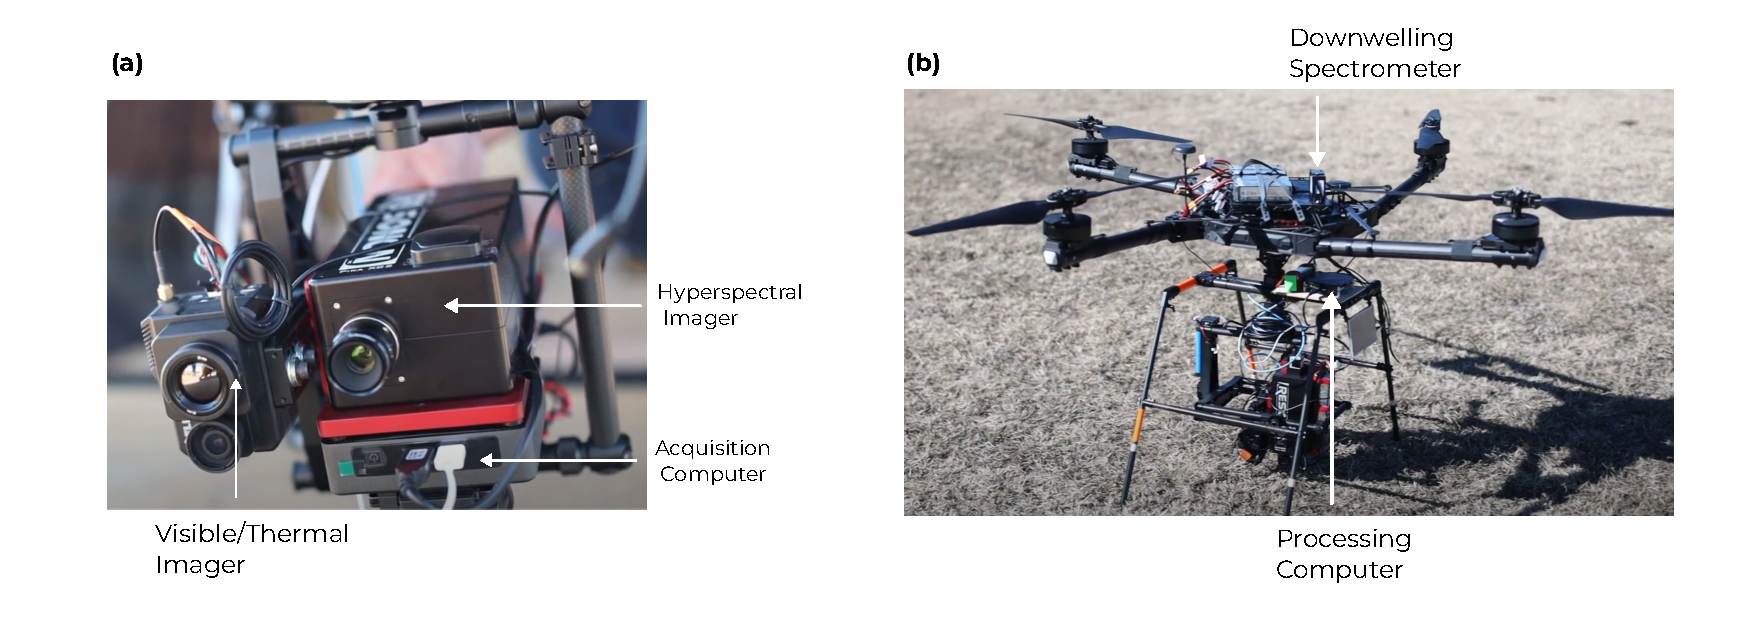
\includegraphics[width=\columnwidth]{figures/materials-and-methods/annotated-drone.pdf}
\vspace{-0.2in}
\caption{Configuration of the UAV: (\textbf{a}) The hyperspectral imager and acquisition computer. (\textbf{b}) The assembled UAV with secondary processing computer and (upward facing) downwelling irradiance spectrometer. \label{fig:drone-components}}
\end{figure} 

To effectively utilize the spectra collected by our UAV, we must account for the variability of the incident light that illuminates the water and transform the raw hyperspectral data cubes from their native imaging reference frame to a chosen coordinate system compatible with the data collected by the USV. This procedure is illustrated in Figure~\ref{fig:hsi-pipeline}.

\begin{figure}[H]
%\begin{adjustwidth}{-\extralength}{0cm}
%\centering
\vspace{-0.3in}
\hspace{-6pt}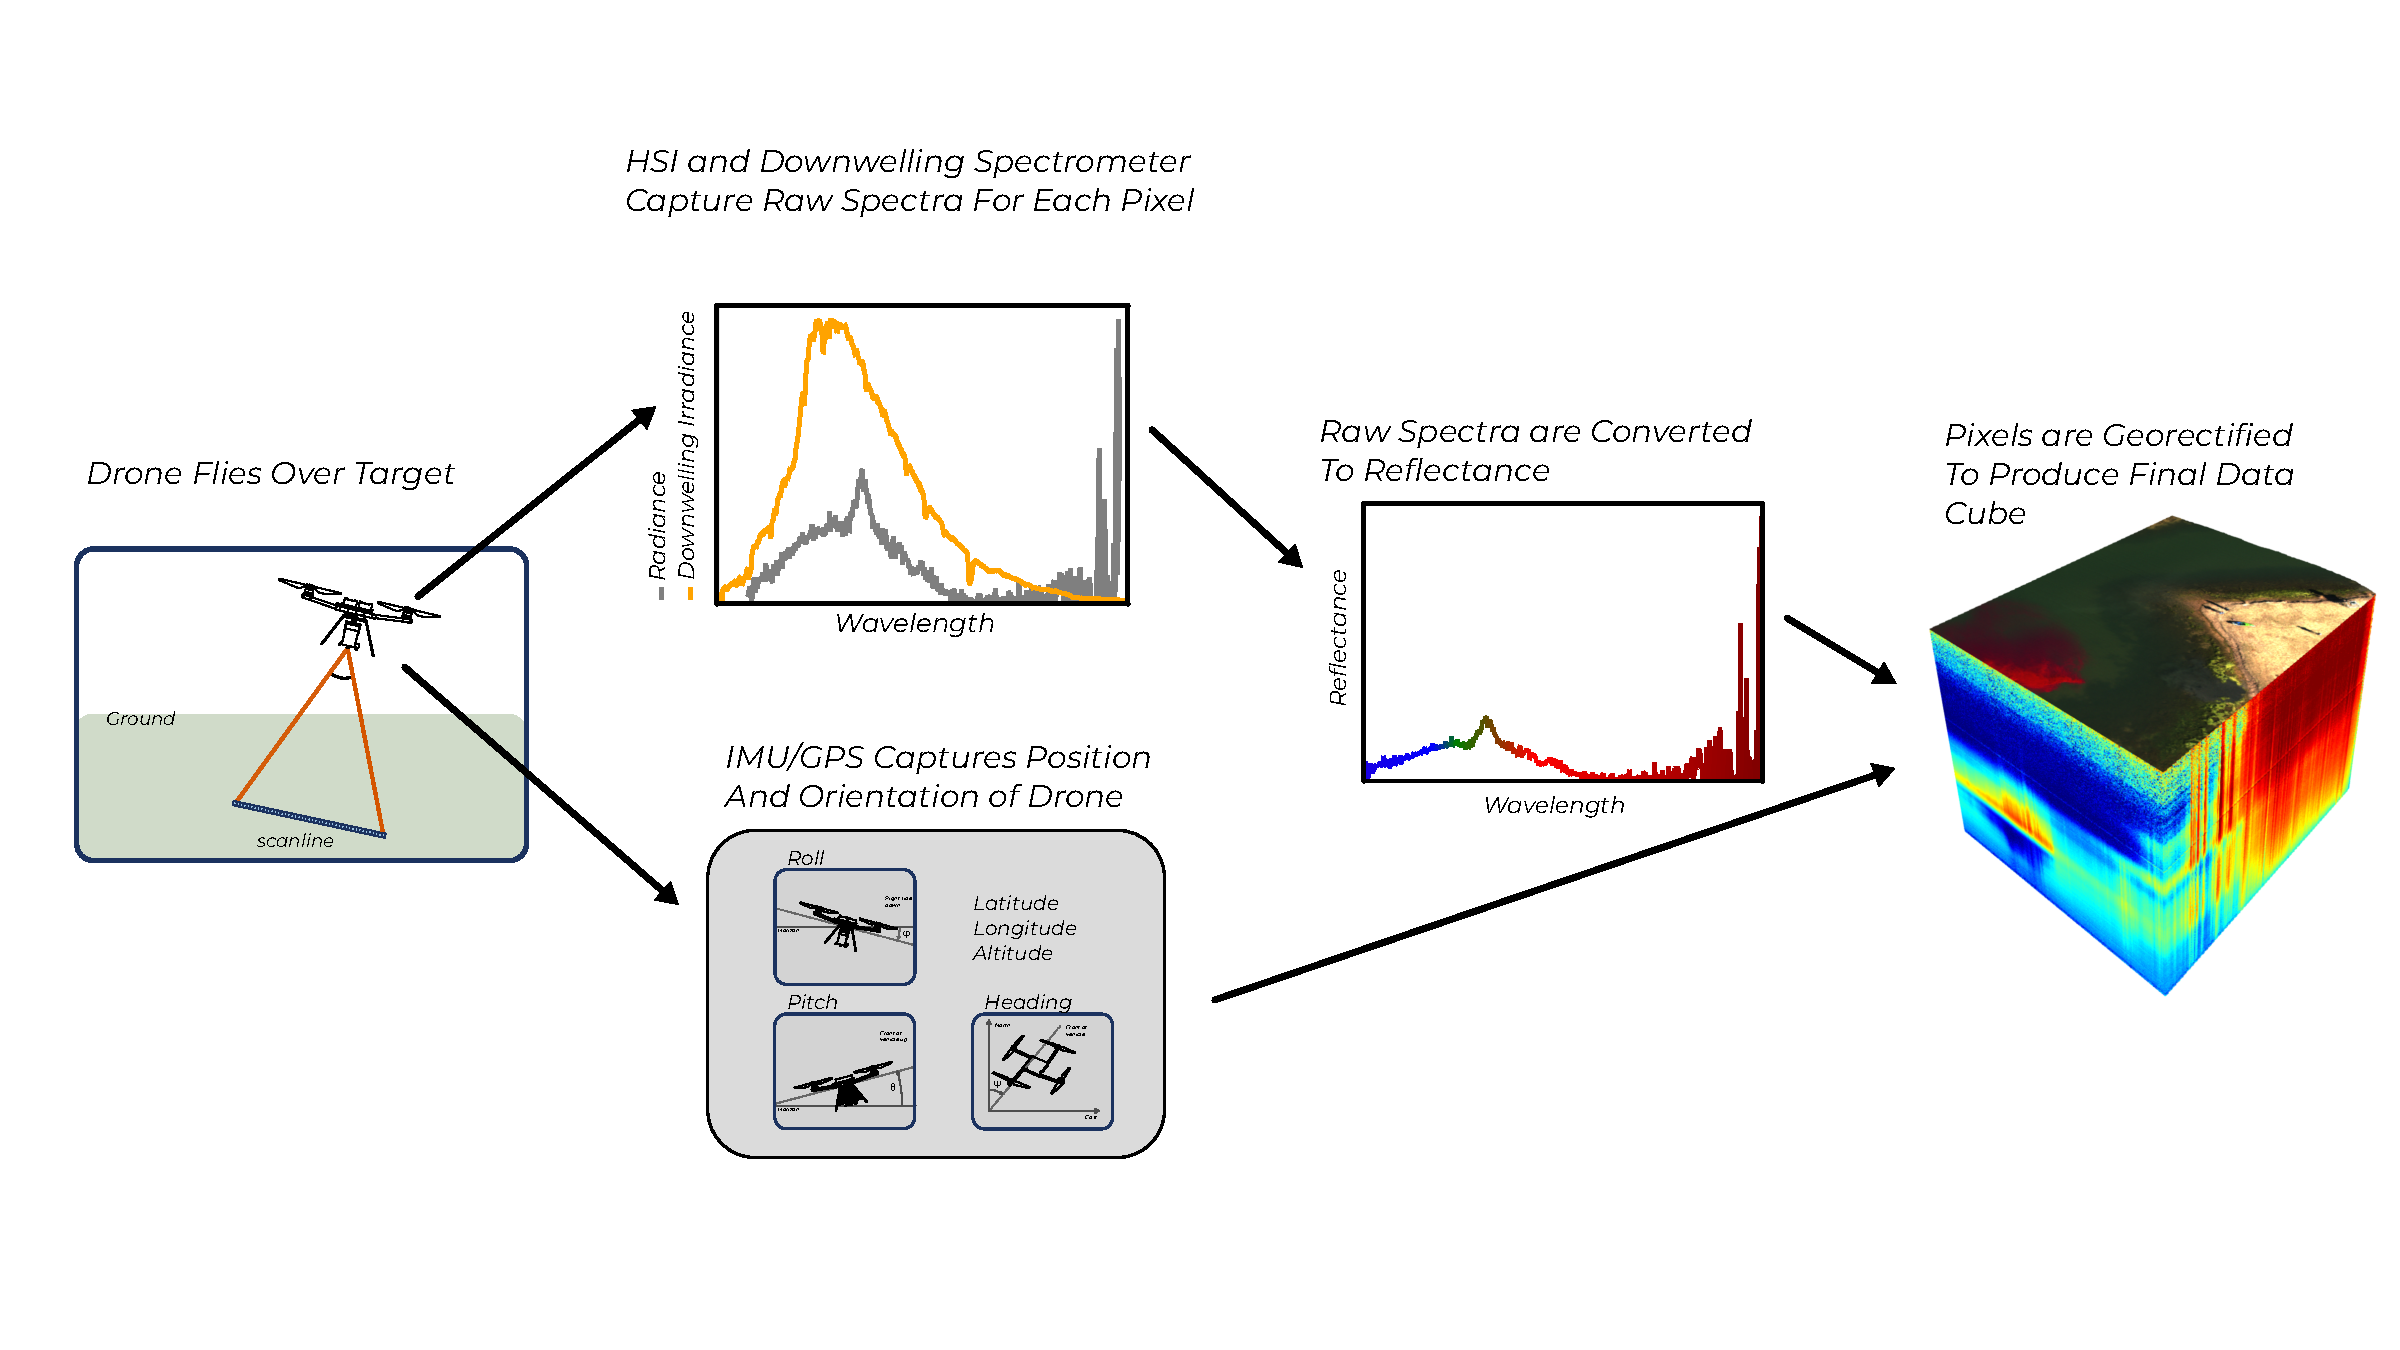
\includegraphics[width=14cm]{figures/materials-and-methods/pipeline-figure-2.pdf}
%\end{adjustwidth}
\vspace{-0.4in}
\caption{Hyperspectral image processing: Hyperspectral data cubes are collected one scan-line at a time (left). By utilizing downwelling irradiance spectra, we convert each pixel from spectral radiance to reflectance. By using orientation and position data from the on-board GPS and INS, we georeference each pixel to assign it a latitude and longitude on the ground. The final data product is the georectified hyperspectral reflectance data cube (right) visualized as a pseudo-color image with reflectance  as a function of wavelength along the z-axis.\label{fig:hsi-pipeline}}
\end{figure}  

The hyperspectral imager utilized in our robot team is in a so-called pushbroom configuration: that is, each image captured by the drone is formed one scan line at a time as the UAV flies. Each scan line consists of 1600 pixels, for which incoming light is diffracted into 462 wavelength bins. In the collection software, a regular cutoff of 1000 lines is chosen so that each resulting image forms an array of size 462 $\times$ 1600 $\times$ 1000 called a hyperspectral data cube. Initially, the captured spectra are in units of spectral radiance (measured in microflicks); however, this does not account for the variability of incident light illuminating the water. To this end, we convert the hyperspectral data cubes into units of reflectance by utilizing the skyward-facing downwelling irradiance spectrometer. When the camera is normal to the water surface, the reflectance is given by
\begin{equation}
    R(\lambda) = \pi L(\lambda)/E_d(\lambda)
\end{equation}
where $L$ is the spectral radiance, $E_d$ is the downwelling irradiance, and a factor of $\pi$ steradians results from assuming the water surface is Lambertian (diffuse) \cite{reflectance-conversion}. 

Having converted the hyperspectral data cube to units of reflectance, we must also georeference each pixel into a geographic coordinate system so that each image pixel can be assigned a latitude and longitude corresponding to the location on the ground from which it was sampled. During our three surveys, the UAV was flown at an altitude of approximately %Please ensure meaning has been retained. 
50 m above the water. At this scale, the surface is essentially flat, so the hyperspectral data cube can be reliably georectified without the need for an on-board digital elevation map (DEM). We adopt the approach outlined in \cite{GeorectificationMuller, GeorectificationBaumker, GeorectificationMostafa} whereby each scan line is georeferenced using the known field of view (30.8$^\circ$) together with the position and orientation of the UAV as provided by the on-board GPS/INS. After a sequence of coordinate transformations, the pixel coordinates are obtained in the relevant UTM zone (in meters). The resulting image is then re-sampled to a final output resolution. For these collections, a resolution of 10 cm was utilized; however, this can be adjusted to optimize the processing time and final resolution for real-time applications. Finally, the UTM pixel coordinates obtained are transformed to latitude and longitude for easy comparison with in situ data collected by the USV. The final result is a georectified hyperspectral reflectance data cube. In Figure~\ref{fig:hsi-infographic}, we visualize one such data cube, highlighting a selection of exemplar pixel spectra as well as the incident downward irradiance spectrum. A pseudo-color image is generated (plotted on the top of the data cube) to illustrate the scene.

\begin{figure}[H]
\begin{adjustwidth}{-\extralength}{0cm}
\centering
\vspace{-0.1in}
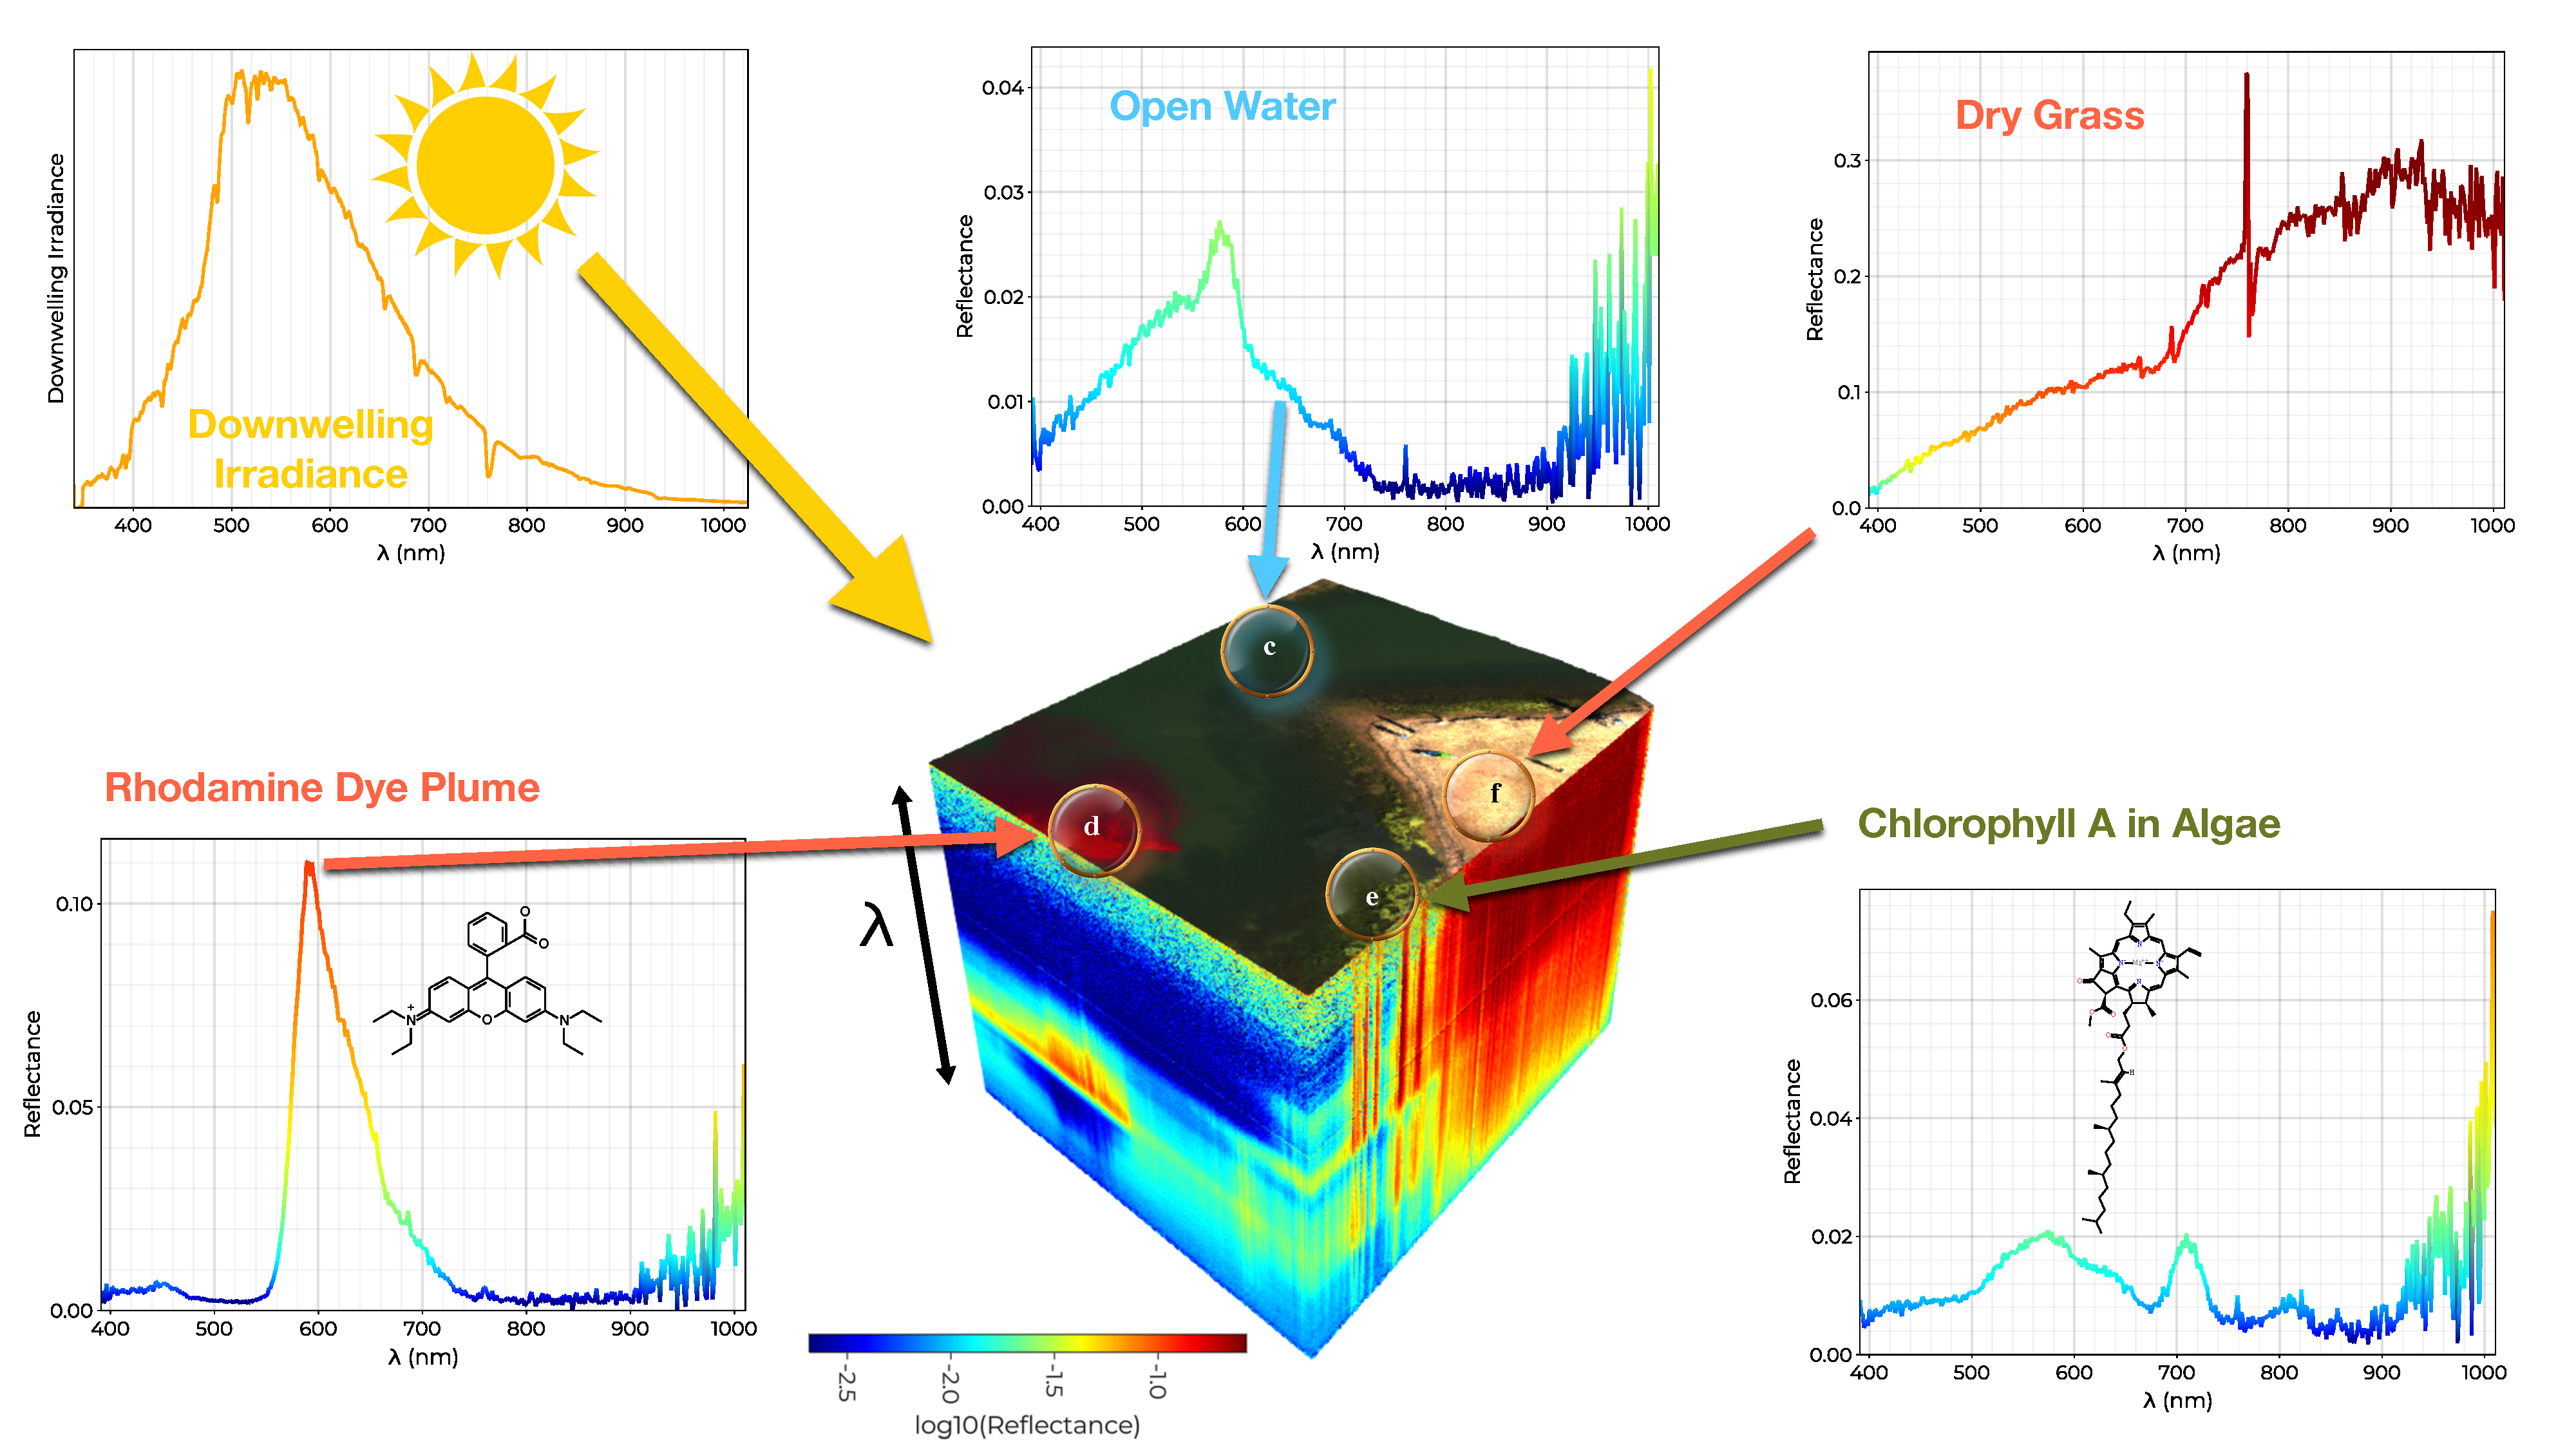
\includegraphics[width=15.5cm]{figures/materials-and-methods/HyperSpectralInfoGraphic.pdf}
\end{adjustwidth}
\caption{A georectified reflectance data cube is visualized (center) with the $\log_{10}$ reflectance along the z-axis and a pseudo-color image on the top. In the top left, we visualize the downwelling irradiance spectrum (the incident light). The surrounding plots showcase exemplar pixel reflectance spectra for open water, dry grass, algae, and a rhodamine dye plume used to test the system.\label{fig:hsi-infographic}}
\end{figure}  

The above processing workflow was implemented using the Julia programming language: a just-in-time compiled language with native multi-threading support \cite{julia-1}. By running this pipeline on the onboard computer, we are able to process the collected hyperspectral data cubes in near real time. This feature is critical for time-sensitive applications wherein we need to quickly assess if an area is safe and cannot afford to wait to download and post-process collected imagery after a flight.

\subsection{Data Collection}

The robot team was deployed at a private pond in Montague, Texas, close to the Oklahoma border for three separate collections on 23 November 2020, 9 December 2020, and 10 December 2020. The pond spans an area $<$0.1 km$^{2}$ and has a maximum depth of 3 m. As shown in Figure~\ref{fig:study-area}, the area includes multiple distinct regions with significant small-scale variability. For each acquisition, the UAV first completed a broad survey of the pond, capturing multiple hyperspectral data cubes. Subsequently, the USV sampled across the pond, collecting in situ reference measurements. Each of these reference measurements was then collocated with individual pixel spectra, whereby the USV track overlapped with the UAV's pixels. To account for any time lag in the values measured by the in situ instruments and to account for the USV's size in comparison to the data cube's spatial resolution, each in situ measurement is associated with a 3 $\times$ 3 grid of HSI pixels: that is, a \mbox{30 cm $\times$ 30 cm} square. These combined data form the tabular dataset on which we train regression models; pixel spectra form input features, and each separate USV sensor forms a distinct target variable.

\begin{figure}[H]
\centering
\vspace{-0.1in}
\hspace{-9pt}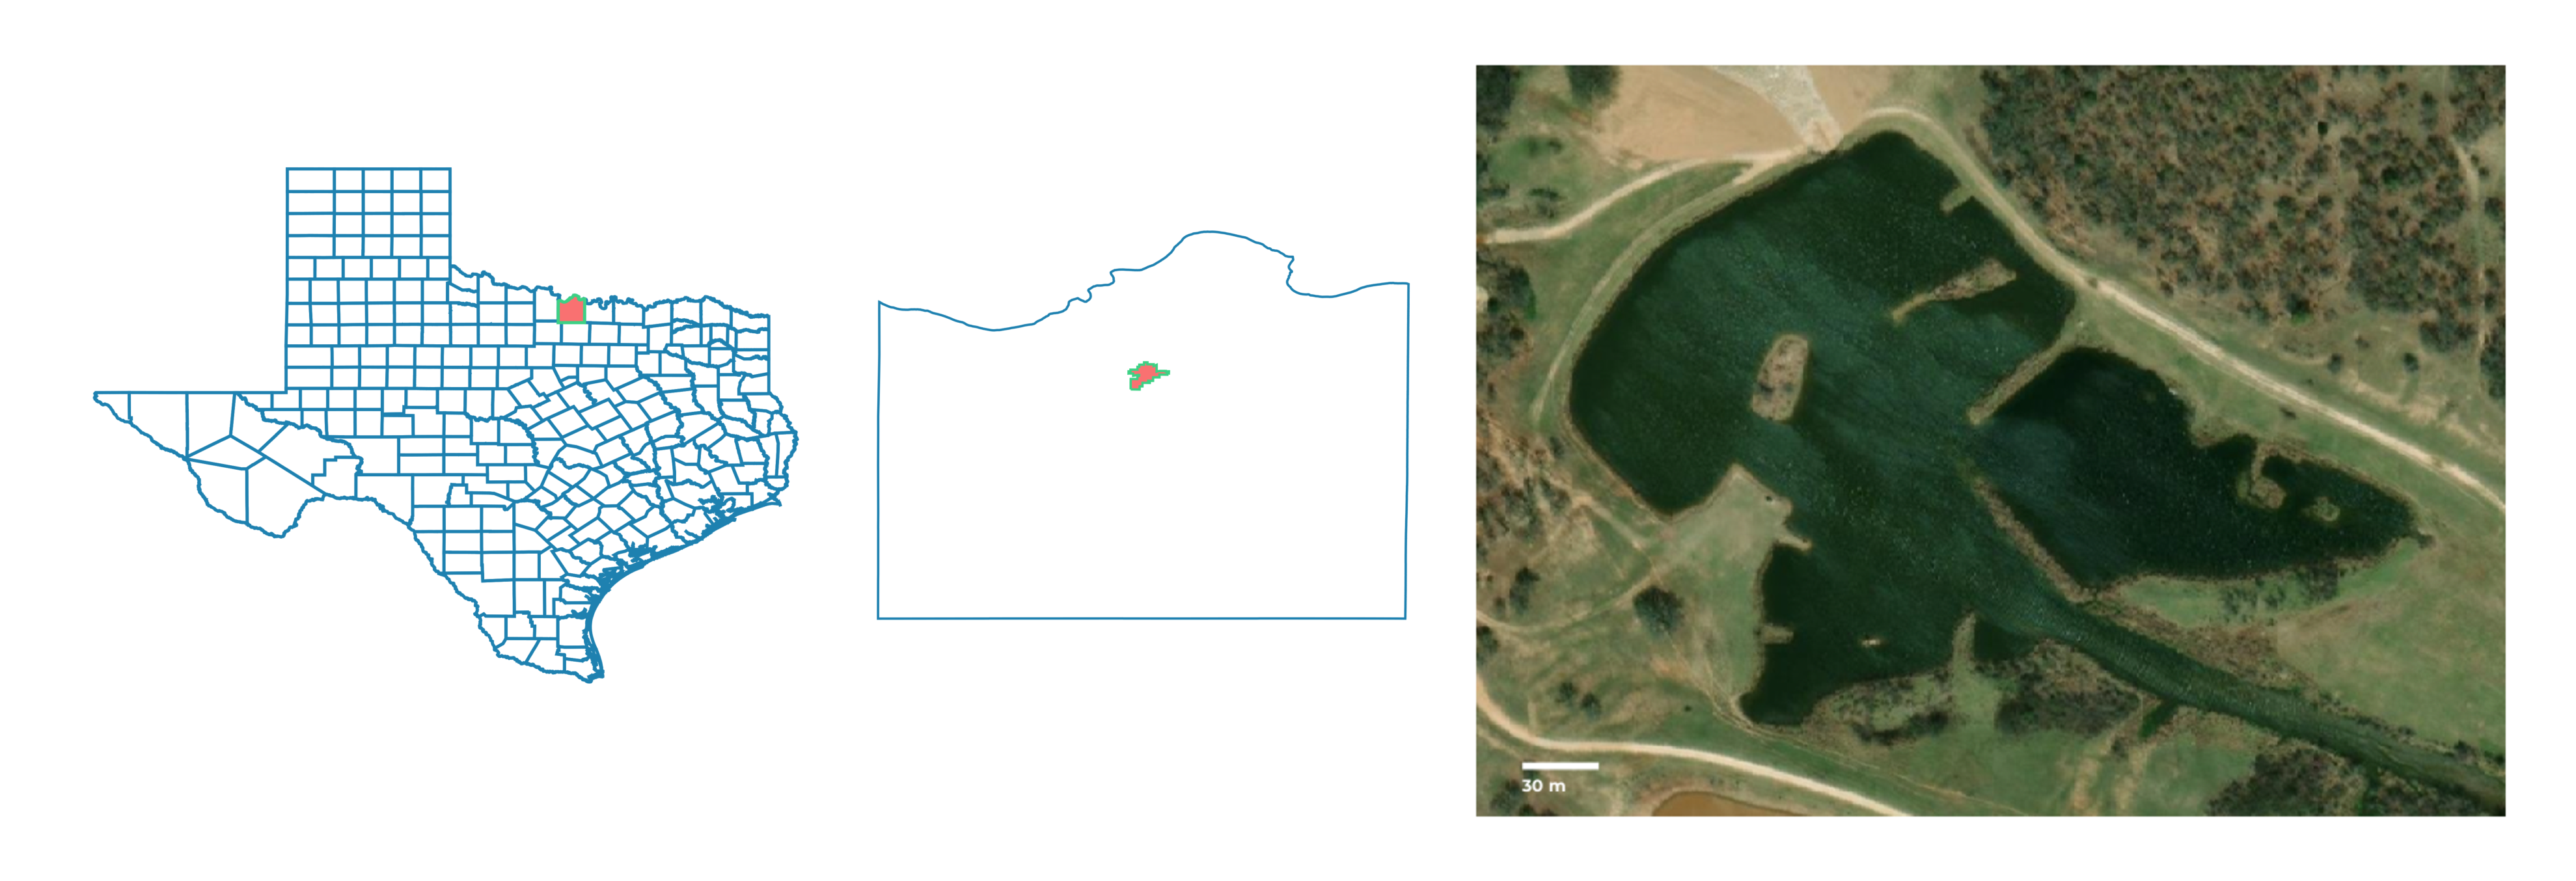
\includegraphics[width=\columnwidth]{figures/materials-and-methods/study-area.pdf}
\vspace{-0.1in}
\caption{The pond in Montague, Texas, where the robot team was deployed. The pond includes multiple distinct regions separated by small islands and grasses. \label{fig:study-area}}
\end{figure}  



Each collection was performed near solar noon to maximize the amount of incident sunlight illuminating the water. For the site in northern Texas, this corresponded to average solar zenith angles of 54.9$^{\circ}$, 56.7$^{\circ}$, and 56.75$^{\circ}$ for 23 November 2020, 9 December 2020, and 10 December 2020, respectively. Given the hyperspectral imager acquires data cubes at nadir, there was little concern for effects due to sunglint. However, to account for any potential variation in lighting conditions between data cubes, we augment the training set with additional features including the drone's viewing geometry (roll, pitch, and heading) and solar illumination geometry (solar azimuth, solar elevation, and solar zenith) as well as the total at-pixel intensity before reflectance conversion, the total downwelling intensity, and the drone's altitude. Further feature engineering is performed to add additional spectral indices that utilize combinations of specific wavelength bands such as the normalized difference vegetation index (NDVI), normalized difference water index (NDWI), simple ratio (SR), photochemical reflectance index (PRI), and more, as outlined in \cite{envi_vegetation_indices, thenkabail2018hyperspectral,kaufman1992atmospherically, SpectralIndexWheat}. A comprehensive list of these added features is provided in Supplementary Table S1. The final dataset includes a total of 526 features (462 reflectance bands plus 64 additional features) with over 120,000 records. 

\subsection{Machine Learning Methods}

For each of the 13 target variables listed in Table~\ref{tab:sensors}, the data were randomly partitioned into a 90:10 training/testing split. To model the data, we chose to use the random forest regressor (RFR) as implemented in the Machine Learning framework for Julia (MLJ) \cite{random-forest-regression, MLJ1}.  Random forests are an ensembling technique based on bagged predictions of individual decision tree regressors trained using the classification and regression trees (CART) algorithm. Each tree in an RFR is trained on a random subset of features and a random subset of training records \cite{decision-tree, random-forest}. Random forests are particularly attractive due to their fast training and inference times. Furthermore, studies continue to observe that tree-based models like random forest remain superior for tabular datasets \cite{grinsztajn2022tree, shwartz2022tabular}.

As reflectance values in adjacent wavelength bins tend to correlate with each other and, therefore, may not necessarily contribute additional information content to the final model, it is desirable to evaluate the relative importance of each feature to the trained model predictions. This is useful both for identifying the most relevant features and for performing feature selection to reduce the final model size. By default, tree-based methods such as RFR allow for impurity-based ranking as described in \cite{random-forest, rfr-importance-ranking}. However, these methods have been shown to be biased towards high cardinality and correlated features \cite{strobl2008conditional}. Therefore, we choose to use the model-agnostic permutation importance as described by \cite{parr2018beware}. To do this, we further partition the training dataset, resulting in an 80:10:10 split with 80\% of the points used for model training, 10\% of the points used for validation and determination of feature importance, and the final 10\% held out as an independent testing set. The importance of the $j^{\text{th}}$ feature is then computed as
\begin{equation}
    \text{Imp}_j = R^2(f(X_{\text{val}}), y_{\text{val}}) - R^2(f(X_{\text{val}}^{(j)}), y_{\text{val}})
\end{equation}
where $(X_{\text{val}}, y_{\text{val}})$ is the validation set, $f(\cdot)$ is the trained model, $R^2(\cdot, \cdot)$ is the coefficient of determination, and $X_{\text{val}}^{(j)}$ is the validation feature set with the $j^{th}$ column randomly permuted. The permutation importance is therefore understood to be the decrease in model performance when the $j^{th}$ feature is replaced by random values from the validation set.

To assess the uncertainty of the final model's predictions, we employed inductive conformal prediction as described in \cite{conformal-prediction-1, conformal-prediction-2, conformal-prediction-3, conformal-prediction-4}. To do this, we computed a set of nonconformity scores of the trained model on the validation set using an uncertainty heuristic: in this case, the absolute error:
\begin{equation}
    s_i = s(X_i, y_i) = \lvert f(X_i) - y_i \rvert = \lvert \hat{y}_i - y_i \rvert
\end{equation}
where $f(X_i)=\hat{y}_i$ denotes the trained ML model applied to the $i^{th}$ calibration record. These n-many scores are sorted, and the interval half width, $d$, is calculated as the $\frac{\lceil(1-\alpha)(n+1) \rceil}{n}$ quantile of this set in order to achieve coverage of $1-\alpha$ on the calibration set. Prediction intervals for new data are then formed as $f(X)\pm d$. For this study, we chose $\alpha=0.1$ for coverage corresponding to a 90\% confidence interval.

Using these tools, the training procedure for each model was as follows: First, each model was trained using six-fold cross-validation on the full 526-feature training set with default hyperparameter values. Feature importances for the trained model were then computed, and the top 25 features were identified. A second model was then trained using the same six-fold cross-validation scheme with only these 25 most important features together with hyperparameter optimization using a random search over the number of trees and sampling fraction. The number of trees was optimized, as it has a significant impact on both model performance and inference time. The sampling ratio determines the fraction of training records that each individual tree is exposed to during training. Tuning this parameter helps limit overfitting by increasing the diversity of trees in the ensemble. Additionally, we chose to fix the maximum tree depth to 20 to control the final model size such that each trained model can fit in-memory on the onboard UAV processing computer. The remaining hyperparameters were left to their default values in order to constrain the total optimization space. The performance of each model was evaluated by computing out-of-fold scores for the coefficient of determination as well as the
\begin{align}
    \text{RMSE} &= \sqrt{\frac{\sum\limits_{i=1}^N (\hat{y}_i-y_i)^2}{N}}, \\
    \text{MAE} &= \frac{\sum\limits_{i=1}^N \lvert \hat{y}_i - y_i \vert}{N},
\end{align}
where RMSE is the root-mean-square error, and MAE is the mean absolute error between the true measurements $y_i$ and the predictions $\hat{y}_i$.

Having identified the model with the best out-of-fold performance, we proceeded to train the final hyperparameter-optimized model on the full training set with the associated uncertainty estimated using conformal prediction.  Then, each final model was evaluated on the previously untouched testing set. We visualize model performance across the distribution of the testing data with a scatter diagram and a quantile--quantile plot, for which successful model predictions should lie close to a 1:1 line.

These trained models can then easily be deployed on the onboard processing computer so that during subsequent surveys, target concentrations can be inferred as imagery are collected and processed. The application of each model to the collected hyperspectral data cubes results in a map of the distribution of the water composition across the pond.

%%%%%%%%%%%%%%%%%%%%%%%%%%%%%%%%%%%%%%%%%%
\section{Results}

The final dataset of combined observations from each of the three separate collections contains more than 120,000 individual records. Based on the size of the UAV payload and the available battery capacity, the collection on 23 November 2020 was chosen to cover the broadest possible area, resulting in small horizontal gaps between flight tracks. The collections on 9 December 2020 and 10 December 2020 were designed to complement this collection by sampling a smaller spatial extent with uniform coverage.

The variability of incident lighting conditions for each collection is visualized in Figure~\ref{fig:downwelling-hist}, wherein the distribution of the total downwelling intensity measured by the downwelling irradiance spectrometer across all hyperspectral data cubes is visualized. Despite performing all UAV flights near solar noon, there were differences in the minimum solar zenith angles between collections due to the time of year. Additionally, there was some slight cloudiness during the 9 December and 10 December collections. 

\begin{figure}[H]
\vspace{-0.1in}
\hspace{-9pt}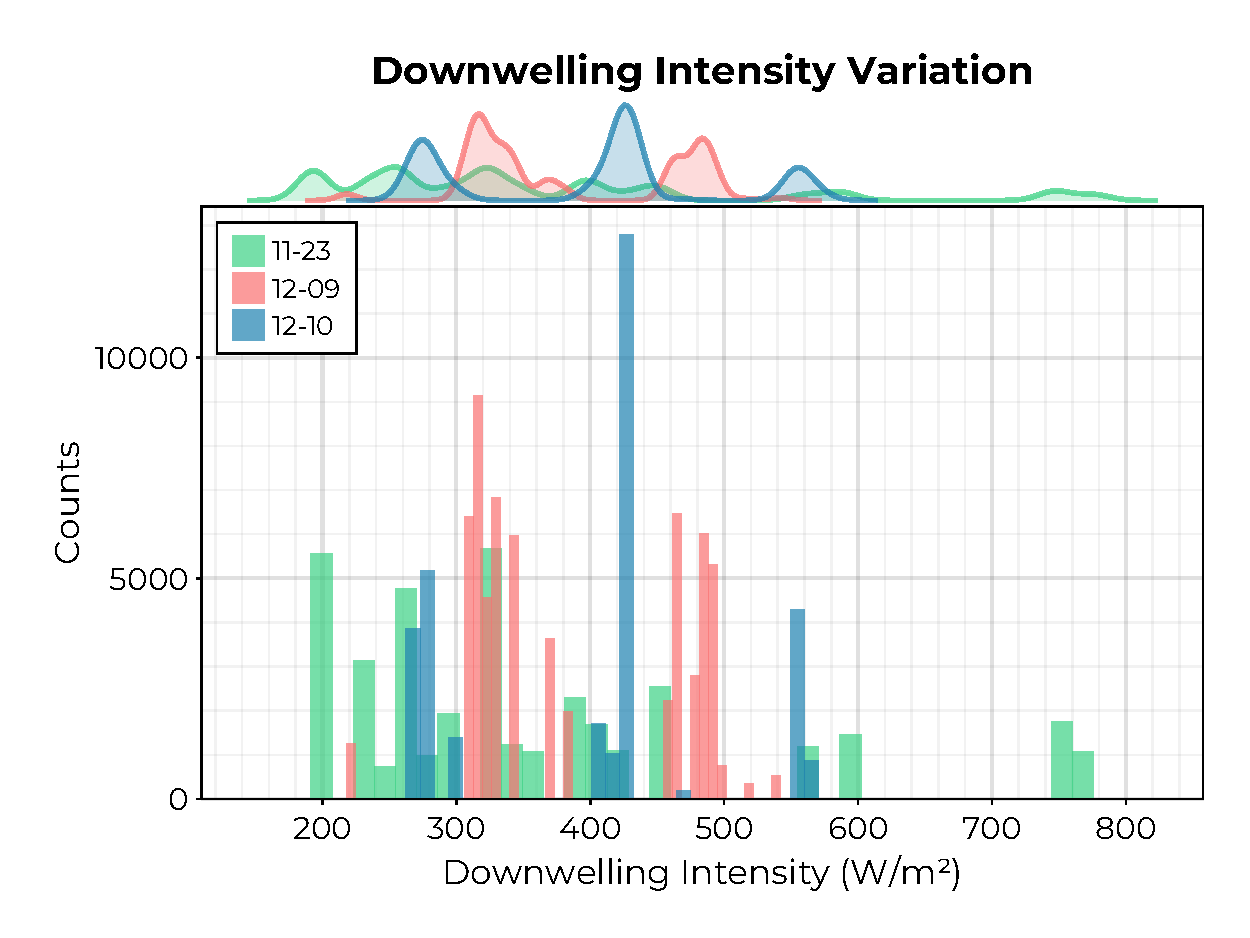
\includegraphics[width=0.7\columnwidth]{figures/results/downwelling-hist.pdf}
\vspace{-0.15in}
\caption{\hl{Distribution} %MDPI: Please use commas to separate thousands for numbers with five or more digits (not four digits) in the picture, e.g., "10000" should be "10,000".
 of total downwelling intensity during each of the three HSI collection flights. The multi-modal nature of these distributions reflects the impact of the relative orientation of the drone to the sun as well as potential occlusion due to the presence of clouds.\label{fig:downwelling-hist}}
\end{figure}   

The results of the model training procedure are presented in Table~\ref{tab:fit-results}. The performance of the model is identified by the $R^2$, RMSE, and MAE out-of-fold estimates (mean $\pm$ standard deviation) of the final hyperparameter-optimized model in the training set, with the target variables ranked in descending order by the $R^2$ value and separated by sensor type (physical variables, ions, biochemical variables, and chemical variables). The final hyperparameter values for each model are listed in Table~\ref{tab:hyperparameters} in Appendix~\ref{Model Hyperparameters}. The small variation in values across folds confirms that the reported performance is independent of how the training set was sampled. Furthermore, we report the interval width that yields a 90\% confidence interval on the holdout validation set determined by the conformal prediction procedure. We then evaluate how the estimated uncertainty generalizes by computing the empirical coverage on the holdout testing set: that is, we compute the percentage of predictions in the test set that actually fall within the estimated 90\% confidence interval. 

From Table~\ref{tab:fit-results},  we see that the empirical coverage achieved by the inferred confidence interval evaluated in the independent test set is within 1\% of our desired coverage for each target modeled. This indicates that the uncertainties obtained by the conformal prediction procedure are reliable---at least within the bounds of the collected dataset. We also note that in all cases, the inferred model uncertainties are larger than the resolution of the in situ sensors. This lends further credence to the inferred uncertainty estimates, as we should not expect to be able to have lower uncertainty than the smallest resolvable difference in reference sensor measurements.

To further examine the differences in model performance between the target variables, we can consider the difference between the RMSE and MAE scores. The MAE is less sensitive to the impact of outliers than the RMSE, and as a consequence, any large difference between the two is indicative of impacts due to the distribution of target values. Indeed, this is the case for turbidity, for which almost all measurements were below 10 FNU, with only a small fraction of observations from a small area near the shore being above this value. %Please ensure meaning has been retained. 
The rest of the models all show mean per-fold RMSE values with sizes comparable to the mean per-fold MAEs. 

In the remainder of this section, we compare the models within each target category.

% \pagebreak

\begin{table}[H] 
\tablesize{\footnotesize}
  \caption{Summary of fitting statistics for each target measurement. Models were evaluated using 6-fold cross-validation on the training set. The estimated uncertainty is evaluated so that a prediction $\hat{y}\pm \Delta y$ achieves 90\% coverage on the calibration holdout set. The empirical coverage is the percentage of predictions in the testing set that fall within the inferred confidence interval. \label{tab:fit-results}}
  \begin{adjustwidth}{-\extralength}{0cm}
  \newcolumntype{C}{>{\centering\arraybackslash}X}
  \begin{tabularx}{\fulllength}{CCCCCCC}
    \toprule
    \textbf{Target} & \textbf{Units} & \textbf{$\text{R}^2$} & \textbf{RMSE} & \textbf{MAE} & \textbf{Estimated Uncertainty} & \textbf{Empirical Coverage (\%)} \\
    \midrule
    Temperature & $^{\circ}$C & 1.0 ± 6.04 $\times$ 10$^{-6}$ & 0.0289 ± 0.000466 & 0.0162 ± 0.00016 &  ±0.039 & 90.3 \\
    Conductivity & $\upmu$S/cm & 1.0 ± 1.54 $\times$ 10$^{-5}$ & 0.574 ± 0.0128 & 0.322 ± 0.00579 &  ±0.76 & 90.6 \\
    pH & 0--14 & 0.994 ± 0.000288 & 0.0145 ± 0.000304 & 0.00739 ± 9.49 $\times$ 10$^{-5}$ &  ±0.017 & 89.5 \\
    Turbidity & FNU & 0.897 ± 0.00611 & 3.13 ± 0.084 & 0.736 ± 0.0156 &  ±1.1 & 89.8 \\
    \midrule
    $\mathrm{Ca}^{2+}$ & mg/L & 1.0 ± 1.06 $\times$ 10$^{-5}$ & 0.285 ± 0.00357 & 0.137 ± 0.00224 &  ±0.33 & 89.8 \\
    $\mathrm{Cl^-}$ & mg/L & 0.995 ± 0.000196 & 0.895 ± 0.0202 & 0.516 ± 0.00759 &  ±1.2 & 90.1 \\
    $\mathrm{Na^+}$ & mg/L &0.993 ± 0.000229 & 6.16 ± 0.102 & 2.83 ± 0.0303 &  ±7.3 & 90.0 \\
    \midrule
    Blue--Green Algae (Phycoerythrin) & ppb & 0.995 ± 0.000601 & 0.783 ± 0.0489 & 0.287 ± 0.00959 &  ±0.73 & 89.3 \\
    CDOM & ppb &  0.965 ± 0.00352 & 0.248 ± 0.0142 & 0.0921 ± 0.0024 &  ±0.15 & 89.9 \\
    Chlorophyll-a & ppb & 0.908 ± 0.00664 & 0.37 ± 0.00934 & 0.131 ± 0.00228 &  ±0.27 & 89.2 \\
    Blue--Green Algae (Phycocyanin) & ppb & 0.708 ± 0.00689 & 0.749 ± 0.0129 & 0.446 ± 0.00405 &  ±0.93 & 89.8 \\
    \midrule
    Crude Oil & ppb & 0.949 ± 0.00267 & 0.247 ± 0.00597 & 0.0935 ± 0.00114 &  ±0.17 & 89.8 \\
    Optical Brighteners & ppb & 0.943 ± 0.00122 & 0.0806 ± 0.0014 & 0.0481 ± 0.000416 &  ±0.095 & 89.8 \\
    \bottomrule
  \end{tabularx}
  \end{adjustwidth}
\end{table}


\subsection{Physical Variables}

Physical variables included temperature, conductivity, pH, and turbidity. In the combined dataset, the distributions for temperature and conductivity had two distinct, nonoverlapping regions corresponding to the measurements from 23 November and the measurements from 9 December and 10 December, respectively. The pH value of the pond was slightly alkaline, showing a multimodal spatial distribution with values ranging from 8.0 to 8.6. As mentioned above, the pond water was very clear for each observation period, with most turbidity values ranging between 1 and 3 FNU and very few above 10.

The results of the hyperparameter-optimized RFR fits are shown in Figure~\ref{fig:physical-fit}. Temperature and conductivity show the best performance in the independent training set, with $R^2$ values of 1.0 (to three decimal places). Similarly, the pH model achieves an excellent fit, with most predictions falling close to the 1:1 line. Quantile--quantile plots for these three models further confirm that the distributions of the true and predicted values match. The turbidity model also achieves a strong fit, with a $R^2$ value of 0.905. The scatter diagram and quantile--quantile plot for this target show that the model performance degrades with larger values, for which deviation in the predicted distribution is apparent past 25 FNU.

\begin{figure}[H]
\vspace{-0.15in}
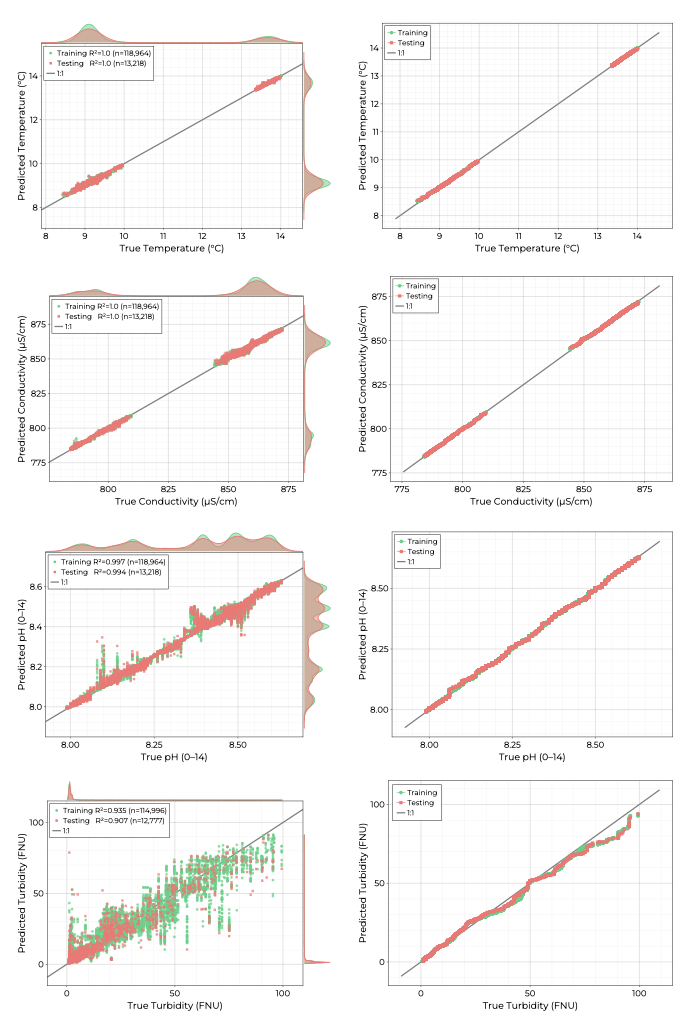
\includegraphics[width=0.9\columnwidth]{figures/results/fits/physical-fitres.png}
\vspace{-0.1in}
\caption{\hl{Scatter} %MDPI: 1. Please change hyphen into endash for range. 2. Please use commas to separate thousands for numbers with five or more digits (not four digits) in the picture, e.g., "10000" should be "10,000". 
 diagrams (\textbf{left}) and quantile--quantile plots (\textbf{right}) for the hyperparameter-optimized RFR models for the physical variables measured by the USV.\label{fig:physical-fit}}
\end{figure}  

The permutation importance of the top 25 features for each of the models of the physical variables is shown in Figure~\ref{fig:physical-fi}. All four models show strong dependence on the solar illumination geometry (solar azimuth, elevation, and solar zenith) as well as the viewing geometry (pitch, altitude, heading, etc.). All four models also include the total downwelling intensity and the total pixel intensity as highly important features. The temperature, conductivity, and pH models all include red-to-infrared reflectance bins and a combination of spectral indices within their most important features. Finally, the turbidity model relies mainly on blue wavelengths from 462 to 496 nm and did not include any spectral indices amongst the 25 most important features.

By applying the trained models to the full hyperspectral data cubes, we can produce maps of the distributions of the target variables as in Figure~\ref{fig:map-physical}. Here, we have chosen to show the map produced from the imagery collected during the 23 November collection period, as it showcases the largest spatial extent. The temperature map shows lower values near the shore, which is to be expected as the air temperature was below the water temperature. The temperature, conductivity, and pH maps all show a distinction between the main body of water and the alcove to the east, which receives little flow from the main body. The turbidity map confirms that the water is largely clear but has elevated levels near the shore.


\begin{figure}[H]

\vspace{-0.15in}
\hspace{-6pt}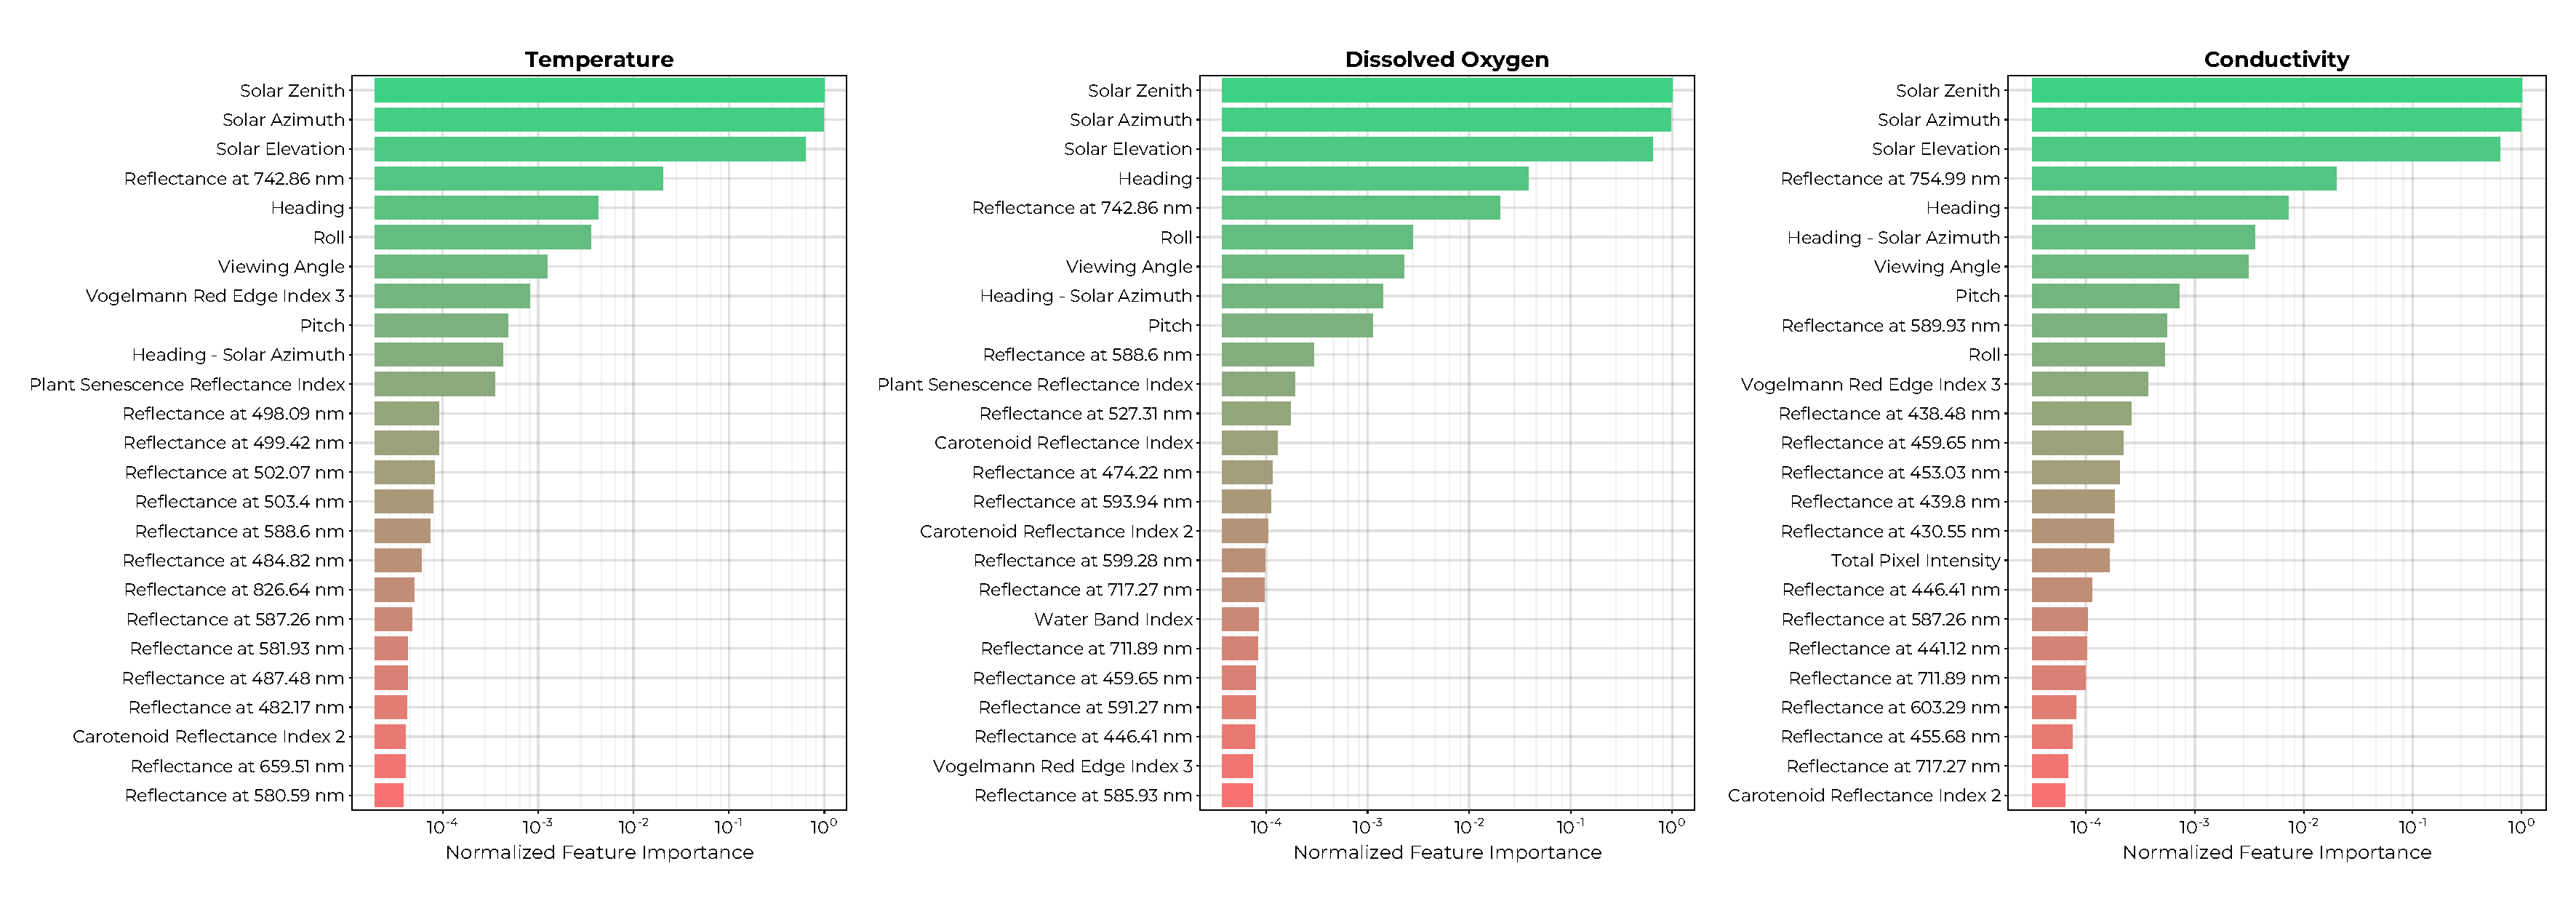
\includegraphics[width=\columnwidth]{figures/results/fits/physical-ranking.pdf}
\vspace{-0.1in}
\caption{Ranked
 \hl{permutation} %MDPI: Please change the hyphen (-) into a minus sign ($-$, "U+2212"). e.g., "-1" should be "$-$1".
 importance for each feature in the physical variable models. Permutation importance measured the decrease in the model's $R^2$ value after replacing each feature in the prediction set with a random permutation of its values.\label{fig:physical-fi}}
\end{figure}  


\begin{figure}[H]

\vspace{-0.15in}
\hspace{-6pt}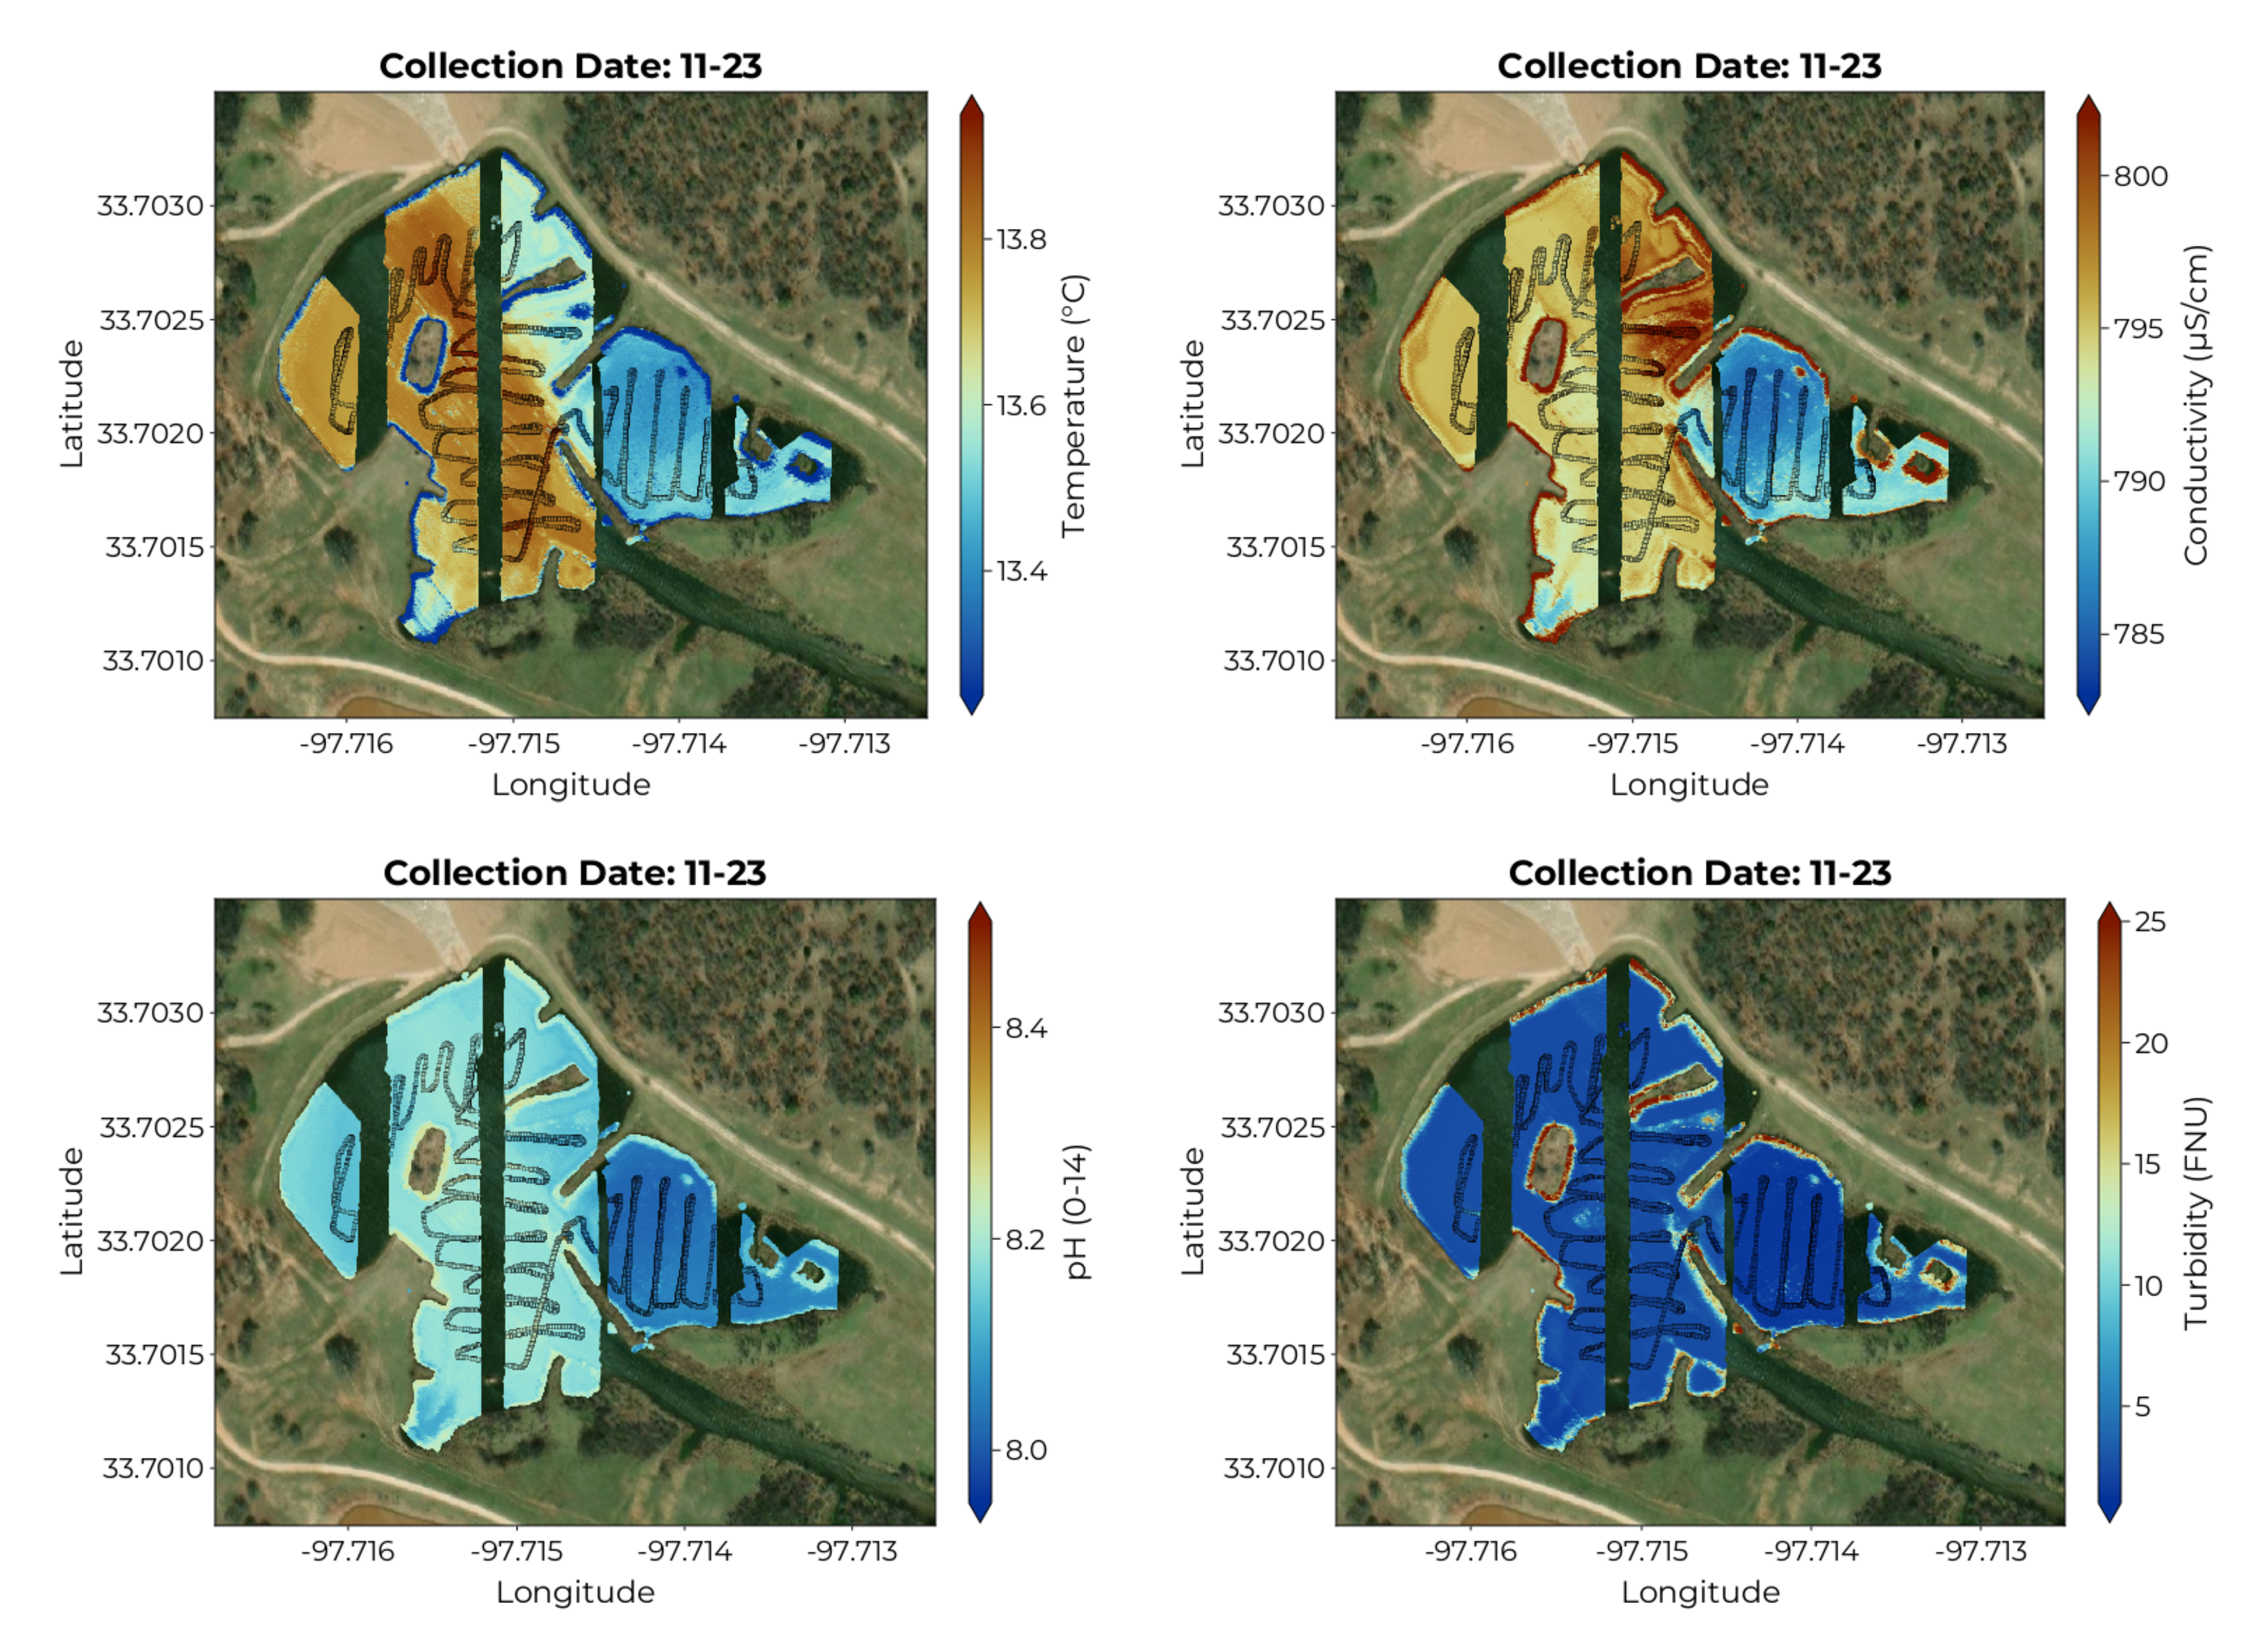
\includegraphics[width=0.9\columnwidth]{figures/results/maps/physical.pdf}
\vspace{-0.05in}
\caption{\hl{Maps} %MDPI: Please change the hyphen (-) into a minus sign ($-$, "U+2212"). e.g., "-1" should be "$-$1".
 generated by applying each of the physical variable models to the hyperspectral data cubes collected on 23 November. Overlaid over the predictions are color-filled squares showing the associated in situ reference data for the same collection period. The size of the squares has been exaggerated for visualization. We note that there is good agreement between the model predictions and the reference data. \label{fig:map-physical}}
\end{figure}  



\subsection{Ions}

The measured ions include $\mathrm{Ca}^{2+}$, $\mathrm{Cl}^{-}$, and $\mathrm{Na}^{+}$. All three measurements showed multimodal spatial distributions throughout the pond on each of the three collections. The scatter diagrams and quantile--quantile graphs for the resulting fits are shown in Figure~\ref{fig:ions-fit}. All three models achieved excellent fits, with $R^2$ values of 1.0, 0.996, and 0.993 on the independent testing set, respectively. Furthermore, there is no clear decrease in model performance for low or high concentrations; rather, for $\textrm{Cl}^{-}$ and $\textrm{Na}^{+}$, the models have the most difficulty in the middle of the target distributions. 

The permutation importance rankings for the top 25 features of each of the ion models is shown in Figure~\ref{fig:ions-fi}. Here, we see that all three models depend on the solar illumination and viewing geometries as well as the total downwelling intensity and the total pixel intensity measured by the hyperspectral imager. All three models utilize a combination of spectral indices that combine green, red, and infrared reflectance bins. The $\textrm{Ca}^{+}$ and $\textrm{Cl}^{-}$ models depend on specific red wavelengths of 740 to 769 nm. $\textrm{Cl}^{-}$ and $\textrm{Na}^{+}$ also depend on green and yellow reflectance bins of 541 to 589 nanometers.

The maps produced by applying the fitted models to the hyperspectral data cubes for 23 November are shown in Figure~\ref{fig:map-ions}. Both positive ions $\mathrm{Ca}^{2+}$ and $\mathrm{Na}^{+}$ show high concentrations in the northwest portion of the pond, with lower values being measured in the alcove on the eastern side. Positive ion concentrations also appear to decrease near the shore. The negative ion $\mathrm{Cl}^{-}$ shows the opposite distribution, with larger values in the alcove to the east and the lowest values on the western side of the pond. The $\mathrm{Cl}^{-}$ ion concentration also appears to increase near the shore.

\begin{figure}[H]

\vspace{-0.15in}
\hspace{-6pt}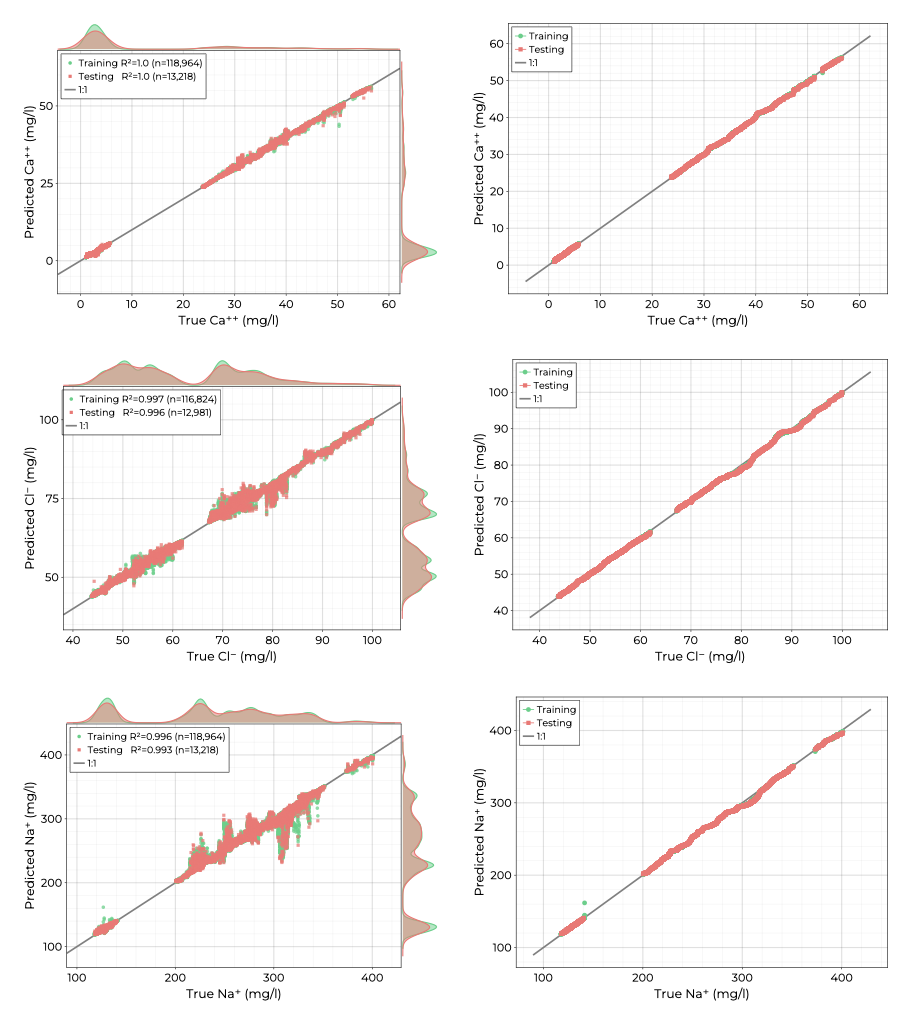
\includegraphics[width=\columnwidth]{figures/results/fits/ions-fitres.png}
\vspace{-0.1in}
\caption{\hl{Scatter} %MDPI: Please use commas to separate thousands for numbers with five or more digits (not four digits) in the picture, e.g., "10000" should be "10,000".
 diagrams (\textbf{left}) and quantile--quantile plots (\textbf{right}) for the hyperparameter-optimized RFR models for the ion measurements made by the USV.\label{fig:ions-fit}}
\end{figure}  

\vspace{-9pt}
\begin{figure}[H]
\begin{adjustwidth}{-\extralength}{0cm}
\centering
\vspace{-0.1in}
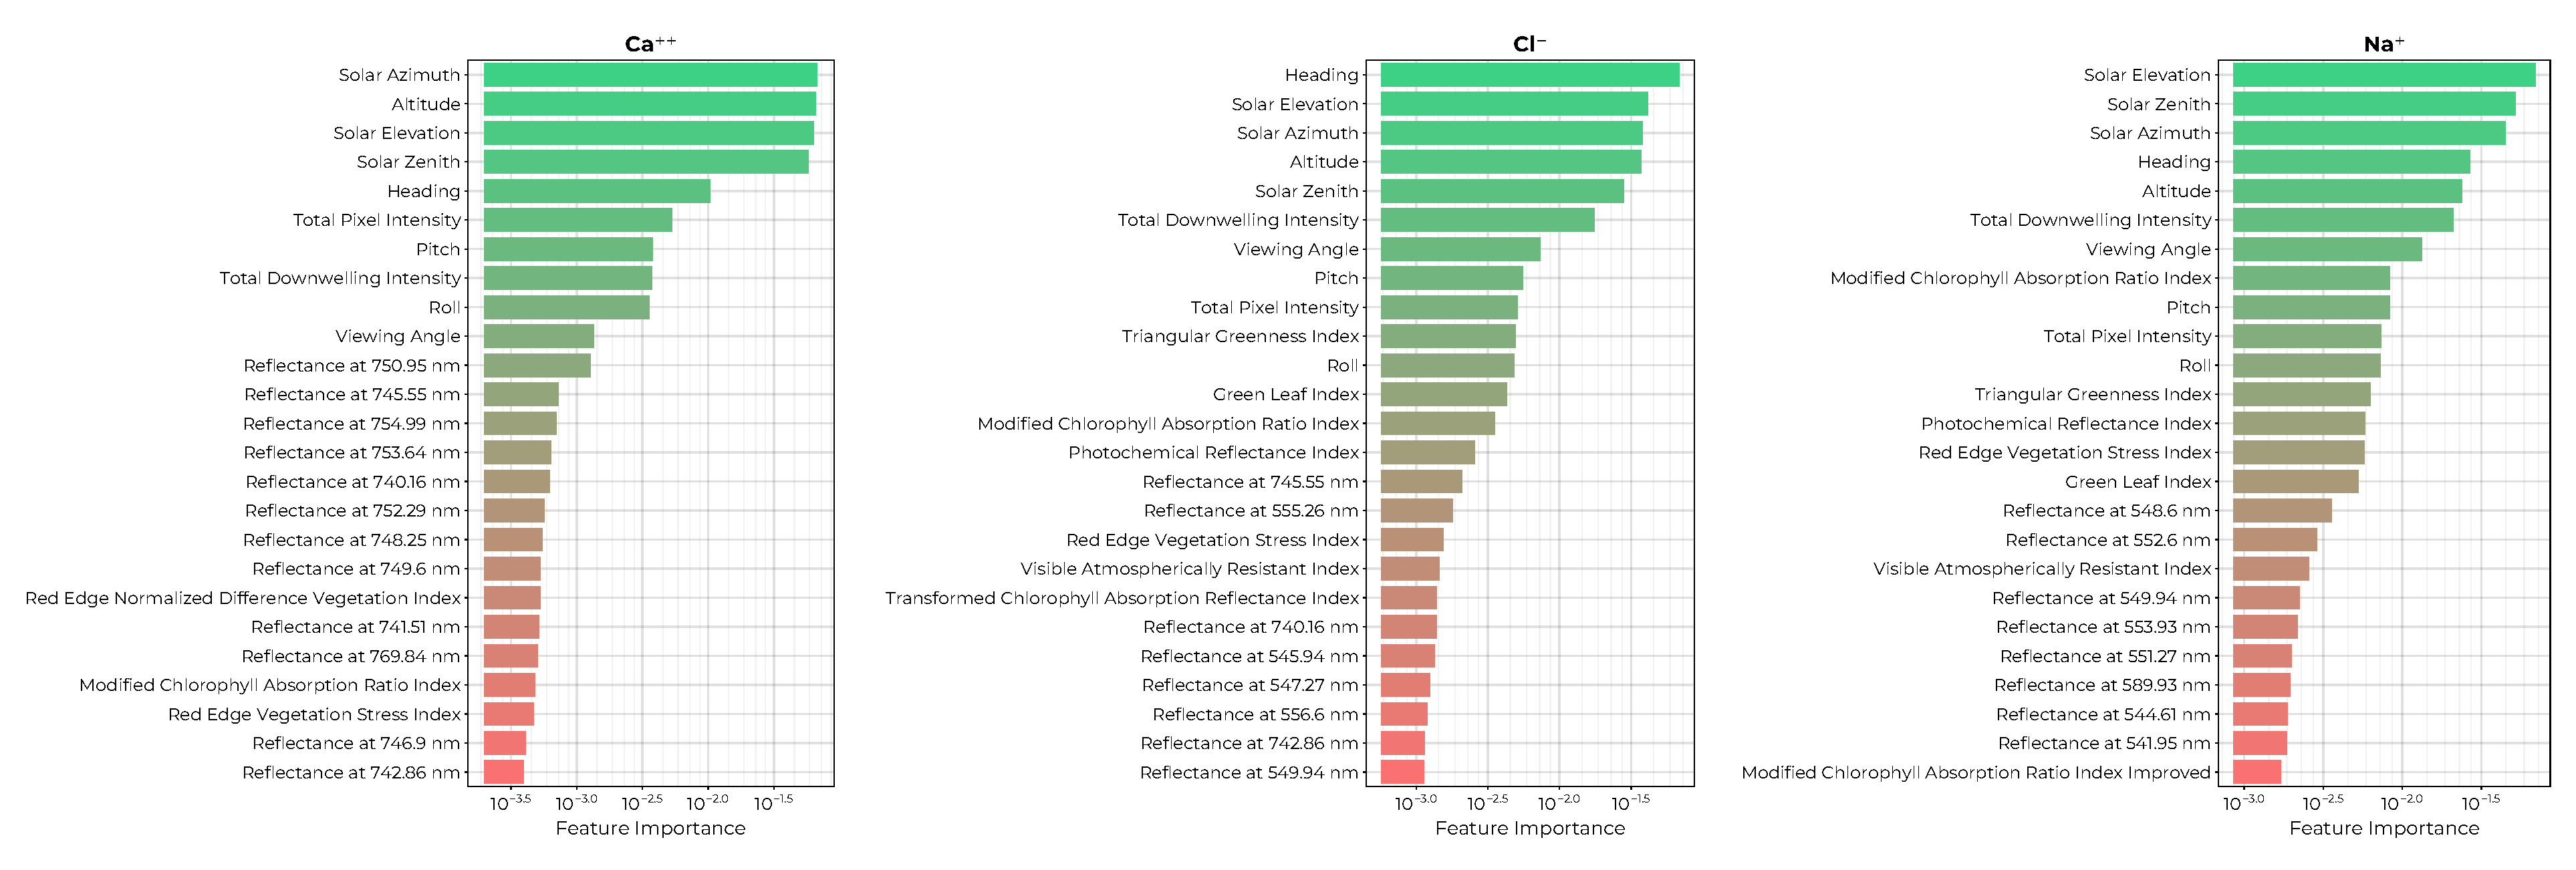
\includegraphics[width=18 cm]{figures/results/fits/ions-ranking.pdf}
\vspace{-0.1in}
\end{adjustwidth}
\caption{\hl{Ranked} %MDPI: Please change the hyphen (-) into a minus sign ($-$, "U+2212"). e.g., "-1" should be "$-$1".
 permutation importance for the top 25 features of the ion models. The permutation importance measures the decrease in the model's $R^2$ value when each feature is replaced by a random permutation of its values.\label{fig:ions-fi}}
\end{figure}  

\begin{figure}[H]

\vspace{-0.15in}
\hspace{-6pt}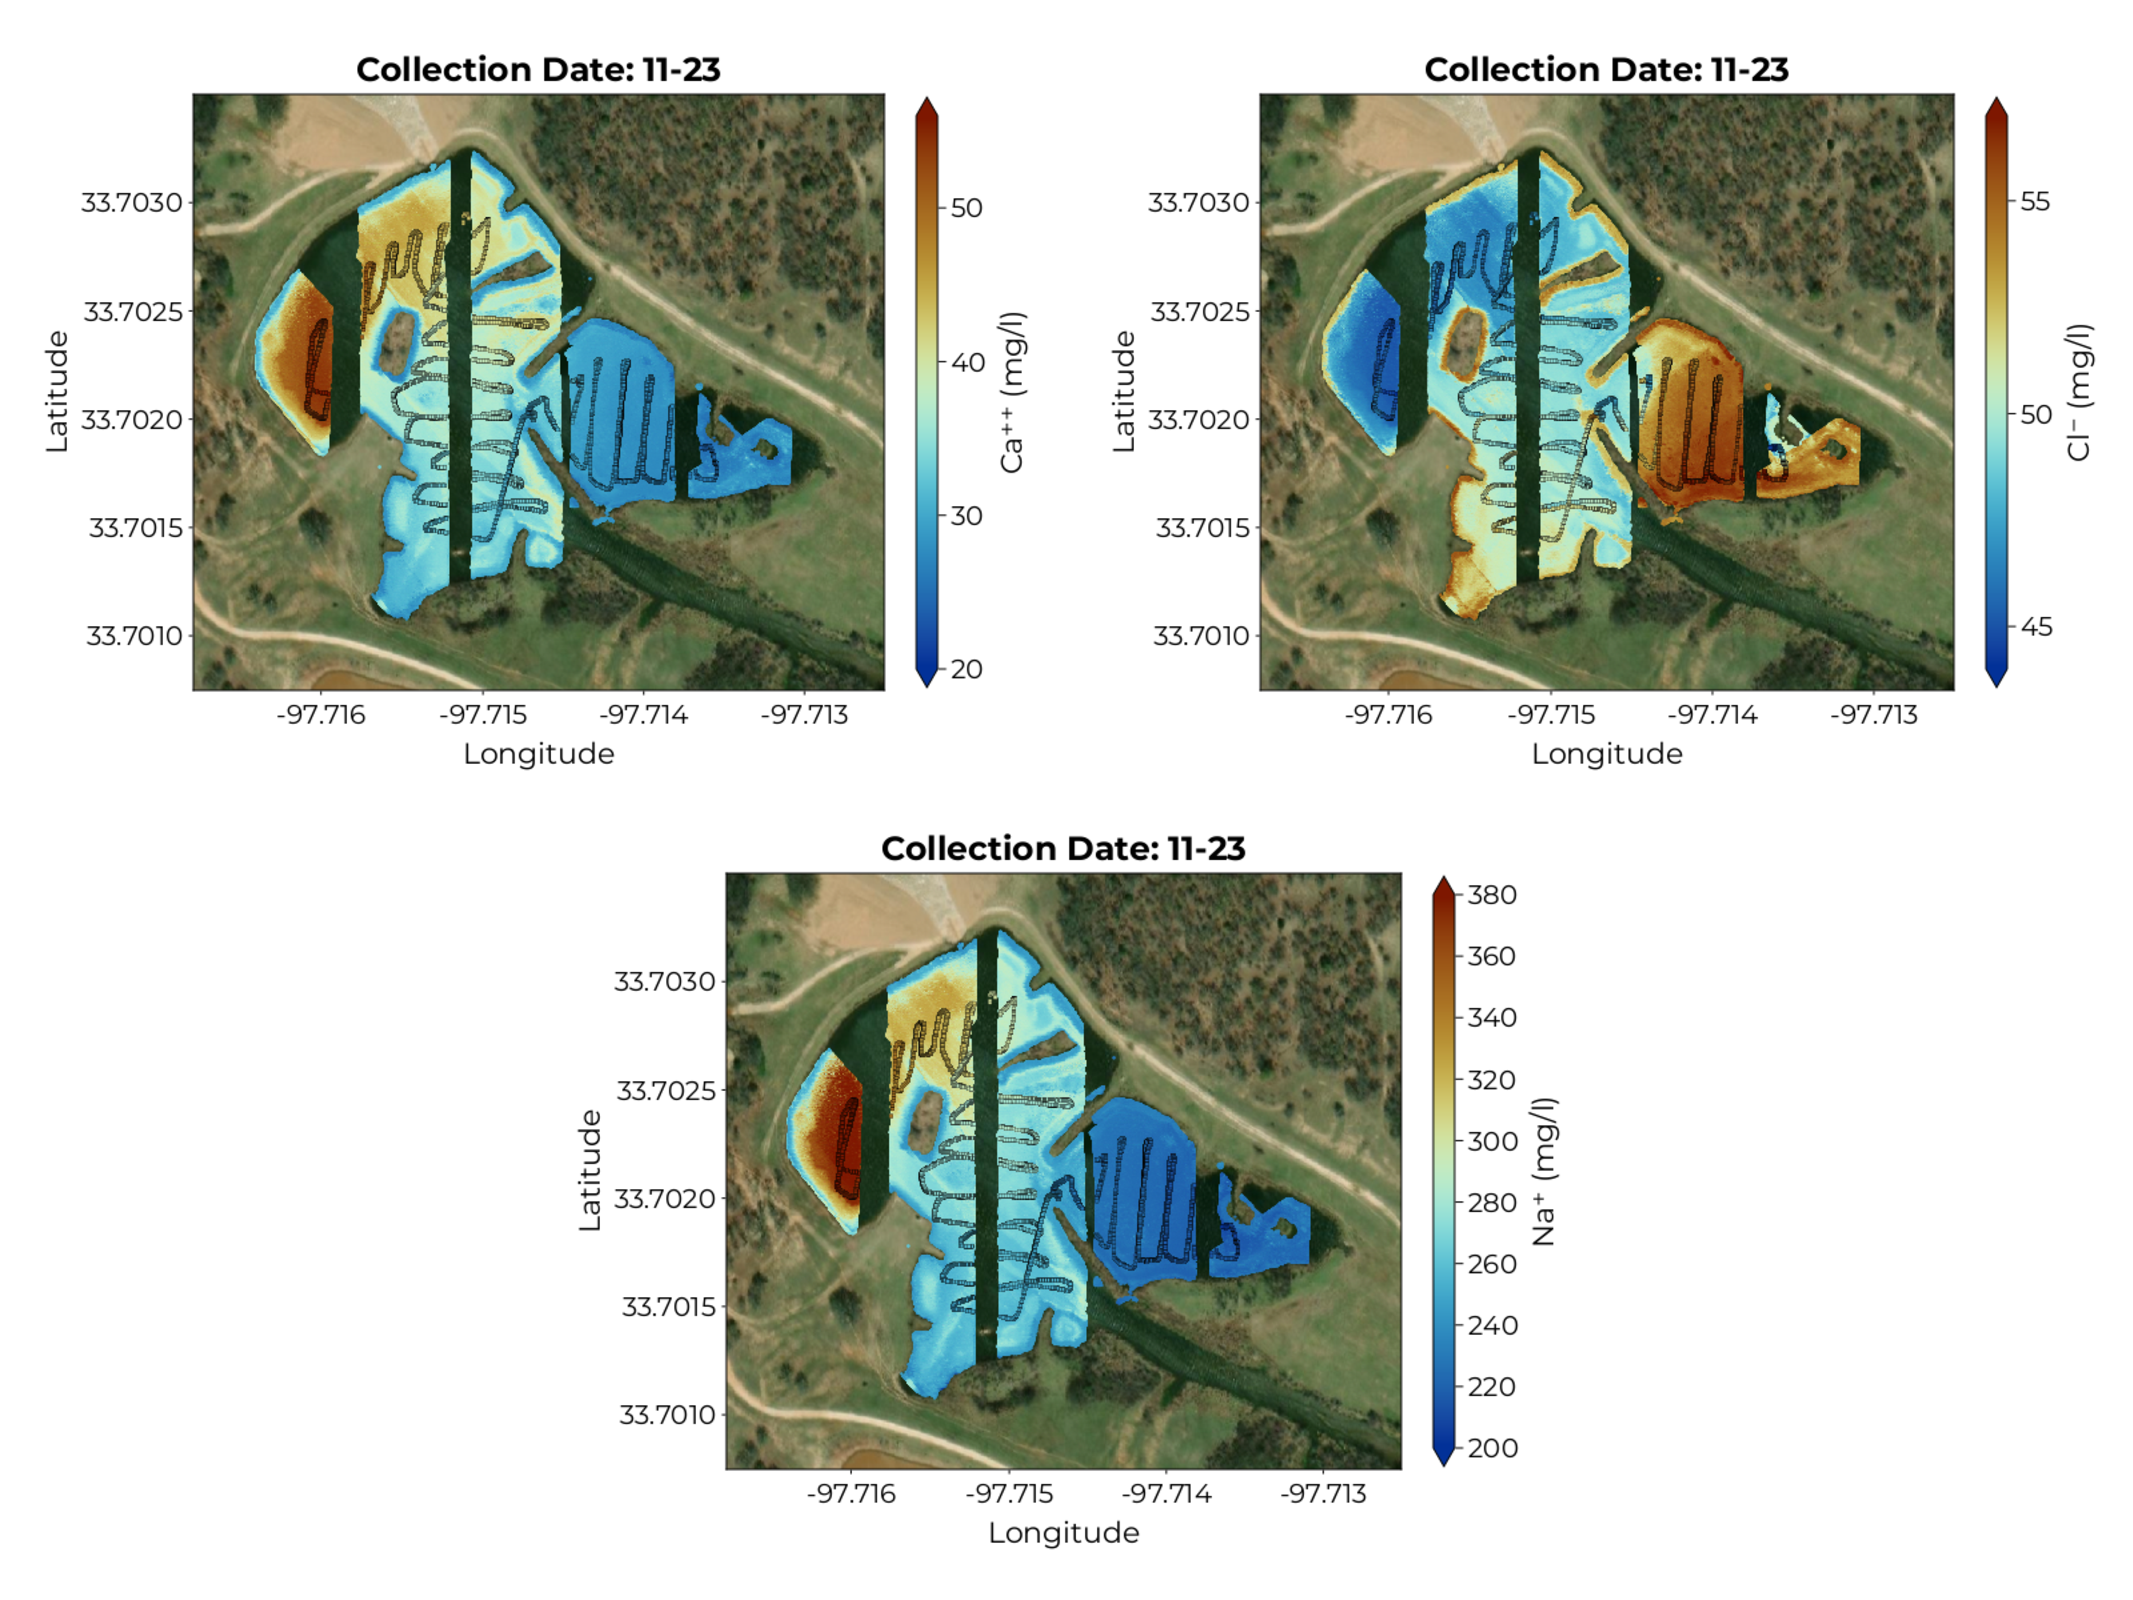
\includegraphics[width=\columnwidth]{figures/results/maps/ions.pdf}
\vspace{-0.1in}
\caption{\hl{Maps} %MDPI: Please change the hyphen (-) into a minus sign ($-$, "U+2212"). e.g., "-1" should be "$-$1".
 generated by applying the trained ion models to the data cubes collected on 23 November. Overlaid on the maps are the in situ reference measurements for the same collection period. The size of the squares has been exaggerated for the visualization. We note that there is good agreement between the generated map and the reference data. \label{fig:map-ions}}
\end{figure}  



\subsection{Biochemical Variables}

The measured biochemical variables include the pigments phycoerythrin, phycocyanin, and chlorophyll-a, as well as CDOM. Phycoerythrin and phycocyanin are both present in blue--green algae, and chlorophyll-a is found in all photosynthetic organisms except bacteria. In the combined dataset, the three pigments showed multimodal distributions separated by the collection day and with little spatial variation within each individual collection. CDOM showed a variable spatial distribution throughout the pond between the main water body and the eastern alcove on 23 November.

The results of the RFR fits for the biochemical variables are shown in Figure~\ref{fig:biochem-fit}. Phycoerythrin showed the best model performance, with an $R^2$ value of 0.995 in the training set. Both CDOM and chlorophyll-a achieved good performance, with $R^2$ values of 0.967 and 0.917 in the training set. Quantile--quantile plots indicate that the CDOM model degrades for values below 16 ppb, where data are sparse. The chlorophyll-a model shows the opposite trend, with poorer performance for concentrations above 5 ppb, for which there are very few records. The phycocyanin model had the lowest performance of the biochemical sensors, with an $R^2$ value of 0.727 and with model predictions rapidly decreasing in quality for concentrations greater than 3 ppb. 

The permutation importance ranking of the top 25 features of each biochemical model is shown in Figure~\ref{fig:biochem-fi}. Again, all four models include the solar illumination and viewing geometries amongst their most important features as well as the total downwelling intensity and total pixel intensity at the imager. Additionally, all four models include some vegetation indices amongst the top features, which utilize combinations of blue, green, yellow, red, and infrared reflectance bands. The phycoerythrin model shows a preference for green reflectance bins from 544 to 556 nm, while the phycocyanin model prefers blue and red reflectance bins. The CDOM model uses mainly red reflectance values, whereas the chlorophyll-a model includes red, green, and blue reflectance bins.

The maps generated for the 23 November collection by applying trained biochemical models are shown in Figure~\ref{fig:map-biochem}. The three pigments show low concentrations in the body of water but elevated levels near the shore. The CDOM distribution shows spatial variability, with higher values in the eastern alcove---similar to the separation seen in the maps for temperature, conductivity, $\textrm{Ca}^{2+}$, $\textrm{Cl}^{-}$, and $\textrm{Na}^{+}$.

\begin{figure}[H]

\vspace{-0.15in}
\hspace{-6pt}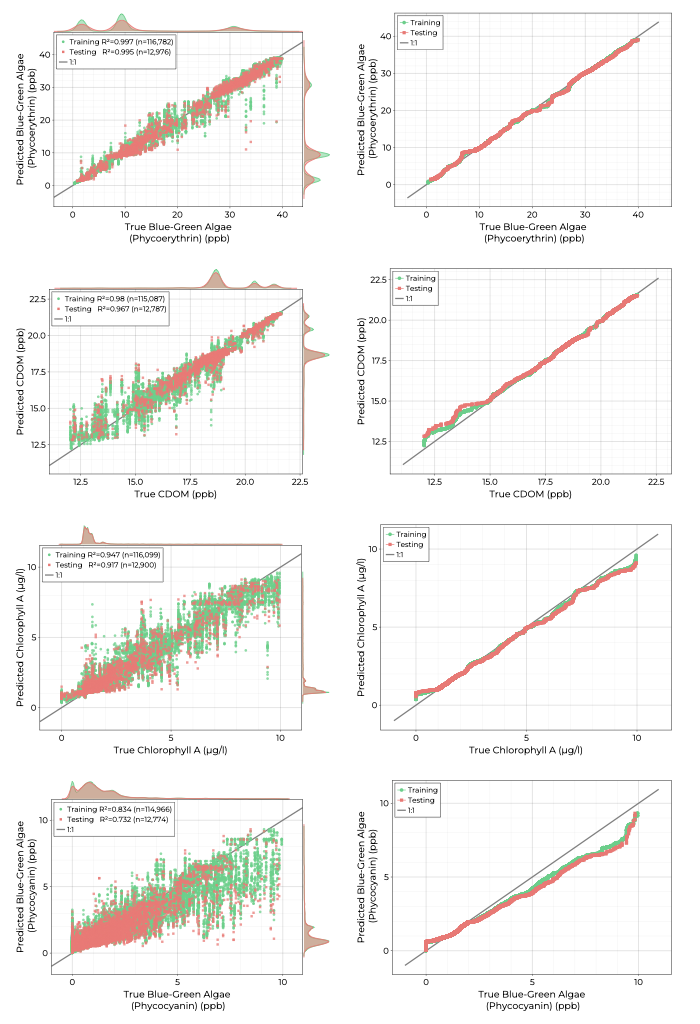
\includegraphics[width=\columnwidth]{figures/results/fits/biochemical-fitres.png}
\vspace{-0.1in}
\caption{\hl{Scatter} %MDPI: Please use commas to separate thousands for numbers with five or more digits (not four digits) in the picture, e.g., "10000" should be "10,000".
 plots (\textbf{left}) and quantile--quantile plots (\textbf{right}) for the final hyperparameter-optimized models for the biochemical targets blue--green algae (phycoerythrin), CDOM, chlorophyll-a, and blue--green algae (phycocyanin). \label{fig:biochem-fit}}
\end{figure}  

\begin{figure}[H]

\vspace{-0.15in}
\hspace{-6pt}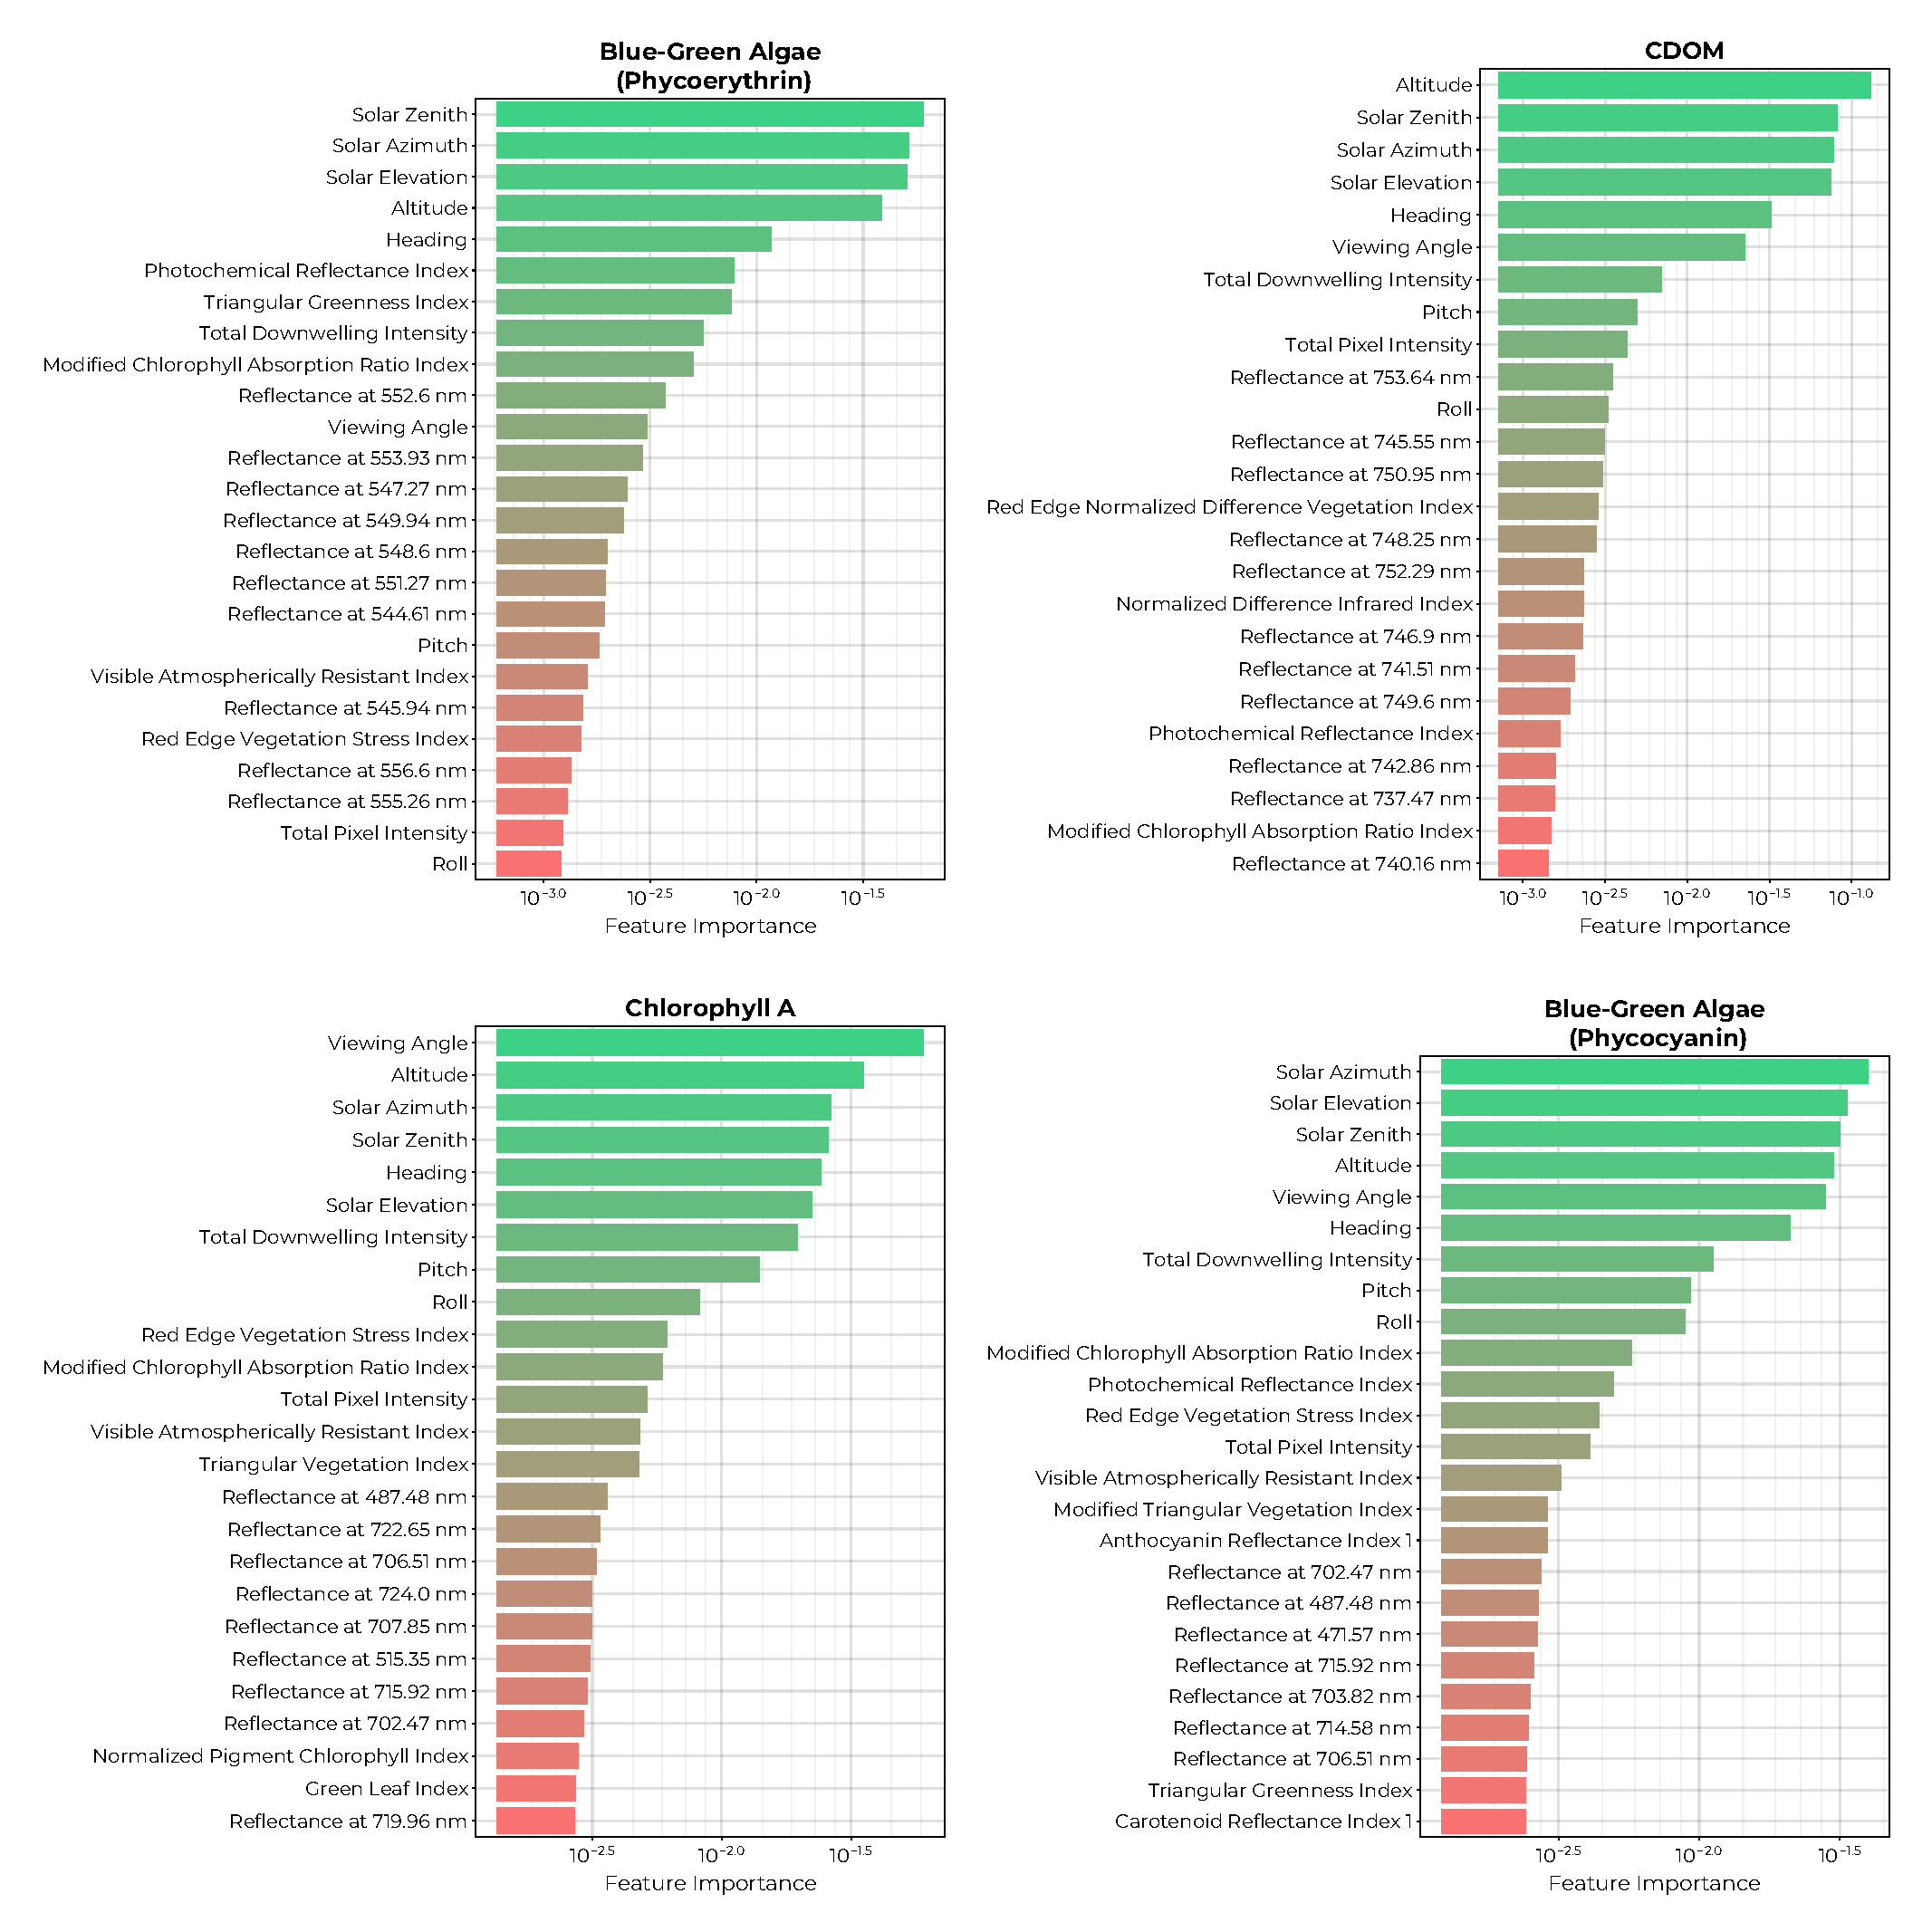
\includegraphics[width=0.9\columnwidth]{figures/results/fits/biochemical-ranking.pdf}
\vspace{-0.1in}
\caption{\hl{Ranked} %MDPI: Please change the hyphen (-) into a minus sign ($-$, "U+2212"). e.g., "-1" should be "$-$1".
 permutation importance for each feature in the trained biochemical models. The permutation importance measures the decrease in the model's $R^2$ value after replacing each feature with a random permutation of its values.\label{fig:biochem-fi}}
\end{figure}  


\vspace{-9pt}
\begin{figure}[H]

\vspace{-0.15in}
\hspace{-6pt}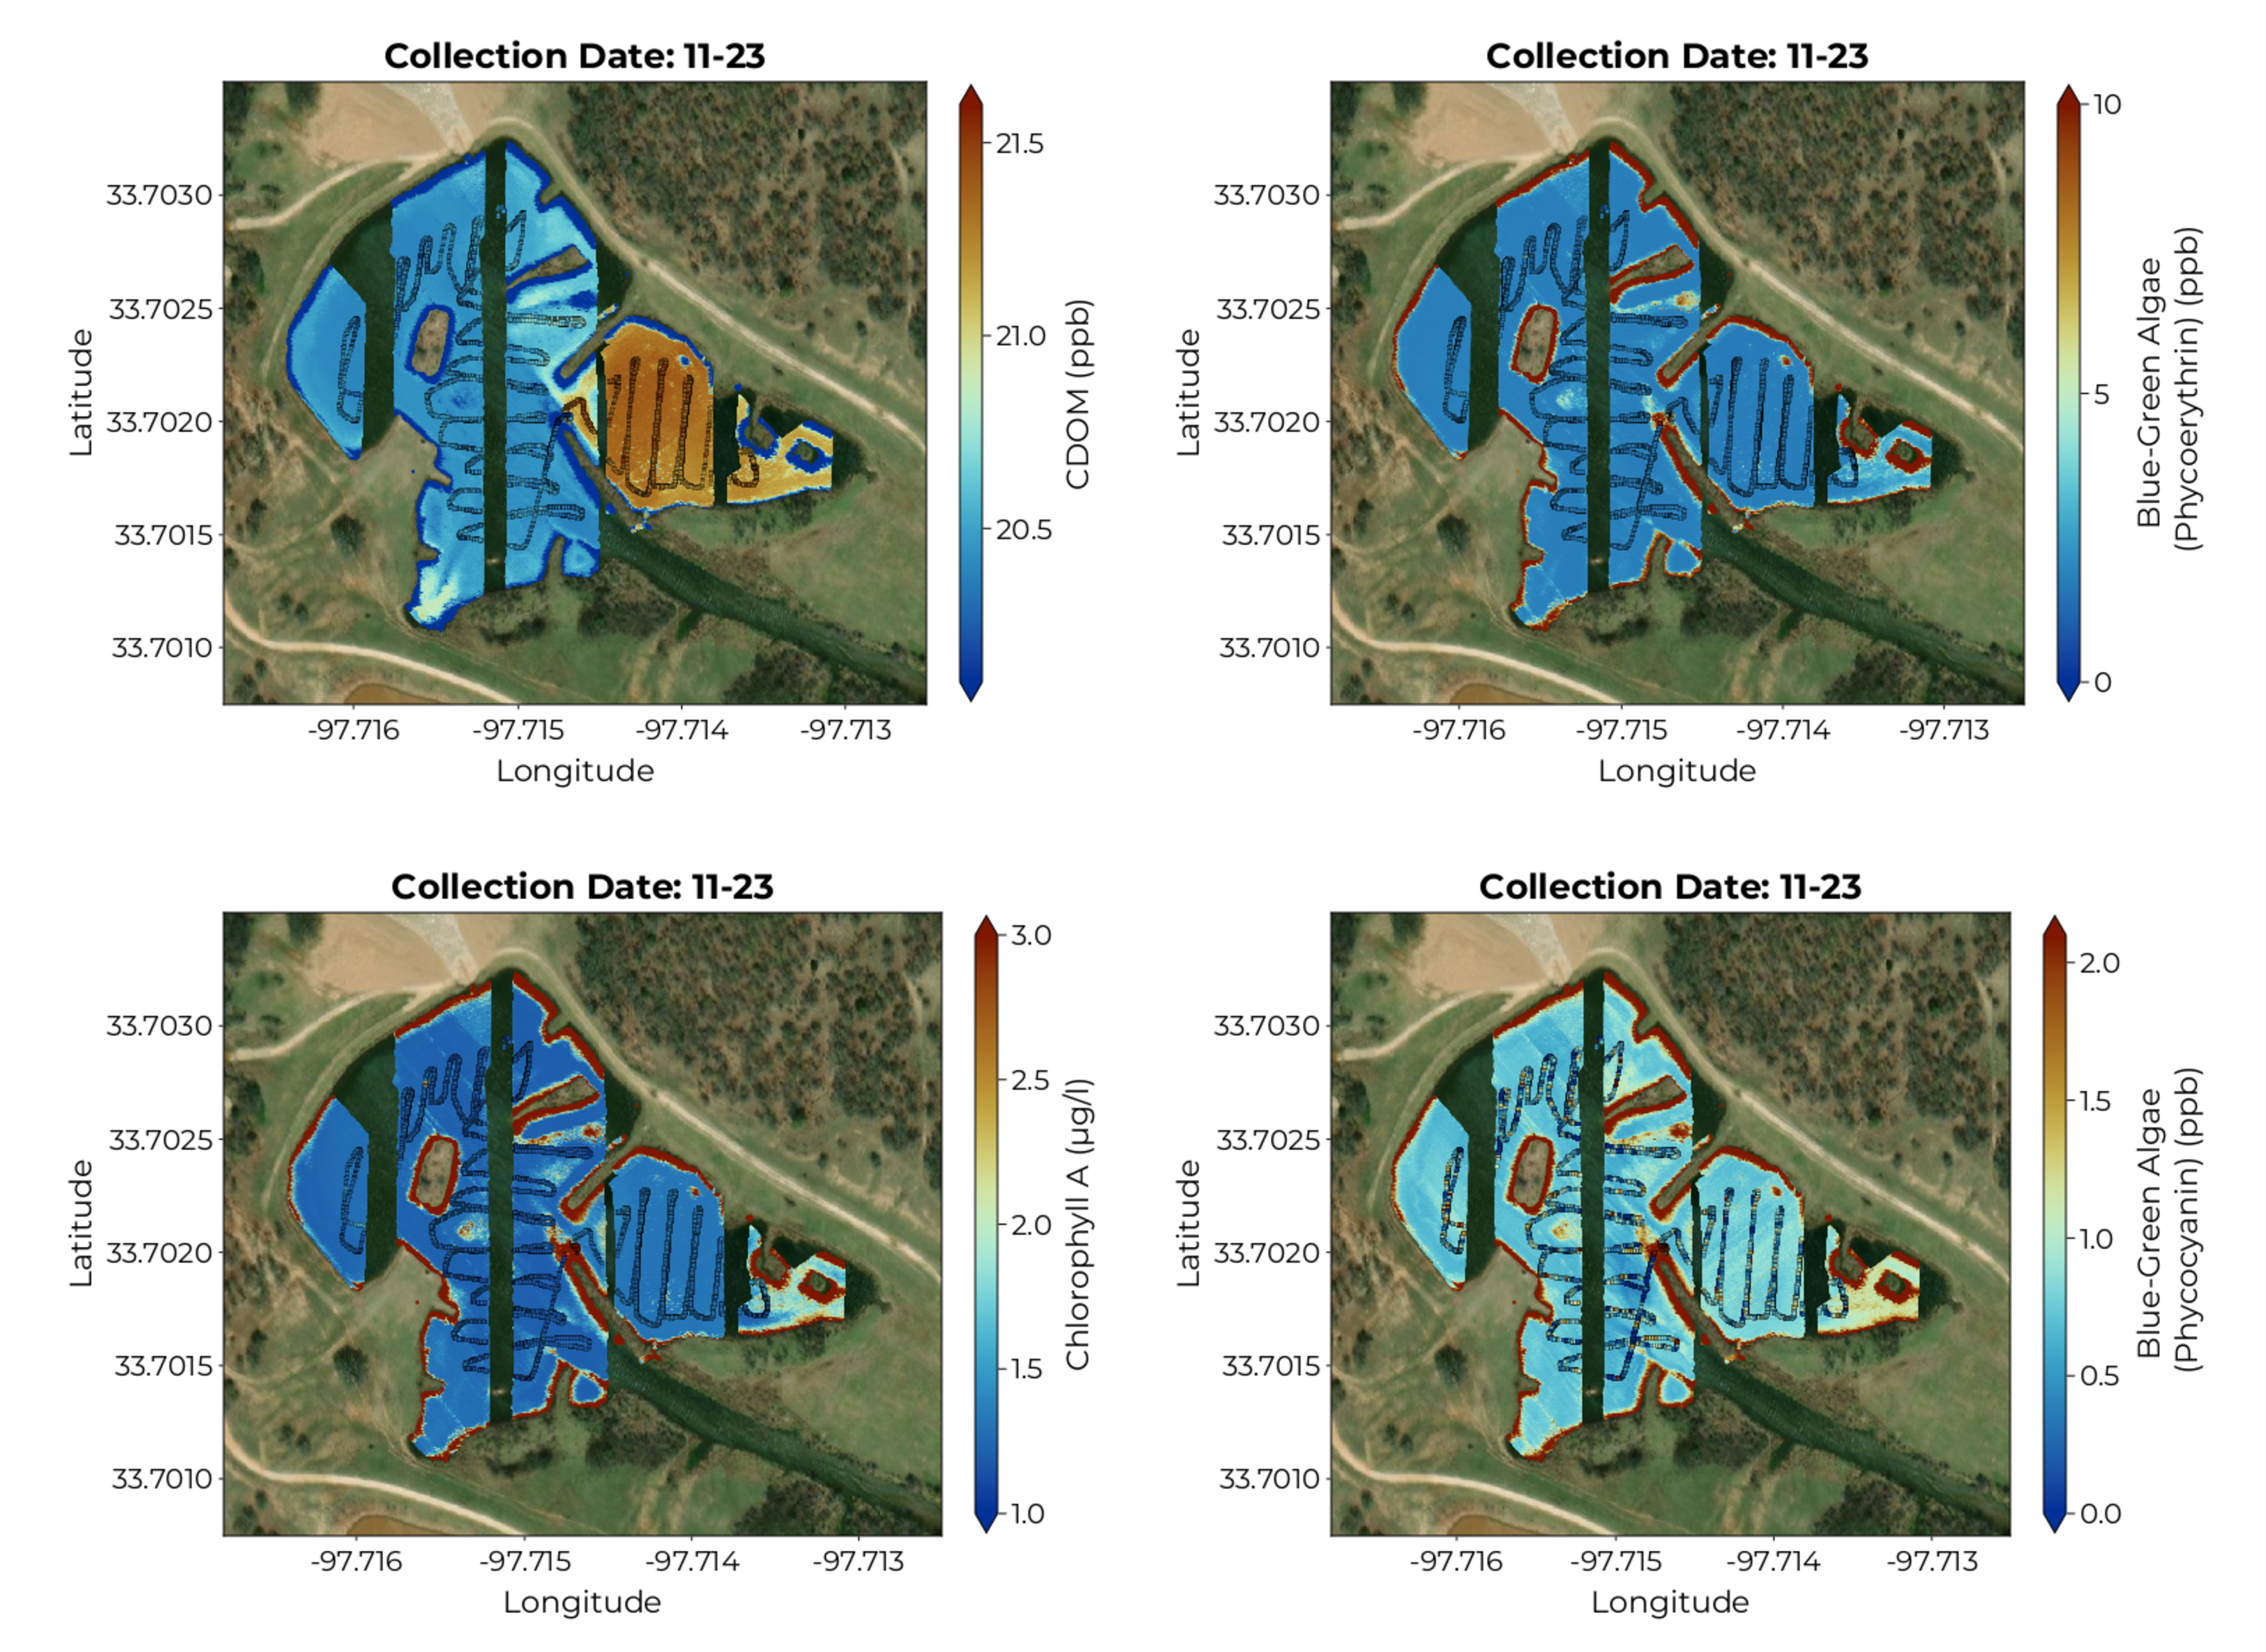
\includegraphics[width=0.92\columnwidth]{figures/results/maps/biochemical.pdf}
\vspace{-0.1in}
\caption{\hl{Maps} %MDPI: Please change the hyphen (-) into a minus sign ($-$, "U+2212"). e.g., "-1" should be "$-$1".
 \hl{generated} %MDPI: There are overlapped content (``longitude} in top and left subfigure). please revise.
 by applying the trained biochemical models to the data cubes collected on 23 November. Overlaid are the in situ reference data for the same collection period. The size of the squares has been exaggerated for the visualization. We note there is good agreement between the predicted map and the reference data. \label{fig:map-biochem}}
\end{figure}  


 

\subsection{Chemical Variables}

The final two models to consider are for the measured chemical concentrations of crude oil (CO) and optical brighteners (OB). The crude oil measurement includes natural unprocessed petroleum, whereas optical brighteners consist of whitening agents that are often added to products such as soaps, detergents, and cleaning agents. Both the crude oil and optical brightener measurements show multi-modal spatial distributions across each collection period. Scatter diagrams and quantile--quantile plots for the fitted models are shown in Figure~\ref{fig:chemicals-fit}. Both models achieve good performance, with $R^2$ values of 0.957 and 0.941 for CO and OB, respectively, %Please ensure meaning has been retained. 
on the holdout test set. The performance of the CO model degrades for concentrations below 24 ppb, for which there are few records. Similarly, the OB model shows worse performance for concentrations below roughly 3.5 ppb.

The ranked permutation importances of the top 25 features for each model are shown in Figure~\ref{fig:chemicals-fi}. Both models rank the solar illumination and viewing geometries together with the total downwelling intensity and total pixel intensities amongst the top features. Both models include a combination of spectral indices using blue, green, yellow, red, and infrared reflectance bins. Additionally, the CO model includes green--yellow reflectances from 539 to 589 nm as well as red reflectances from 749 to 769 nm. The OB model includes yellow reflectance at 584.6 nm and red reflectance bins.

The maps generated by applying the CO and OB models to the 23 November data cubes are shown in Figure~\ref{fig:map-chem}. Both models show a distinct spatial distribution, with elevated values in the eastern alcove of the pond---similar to the CDOM distribution in Figure~\ref{fig:map-biochem}.




% Example of a figure that spans the whole page width. The same concept works for tables, too.
%\begin{figure}[H]
%\begin{adjustwidth}{-\extralength}{0cm}
%\centering
%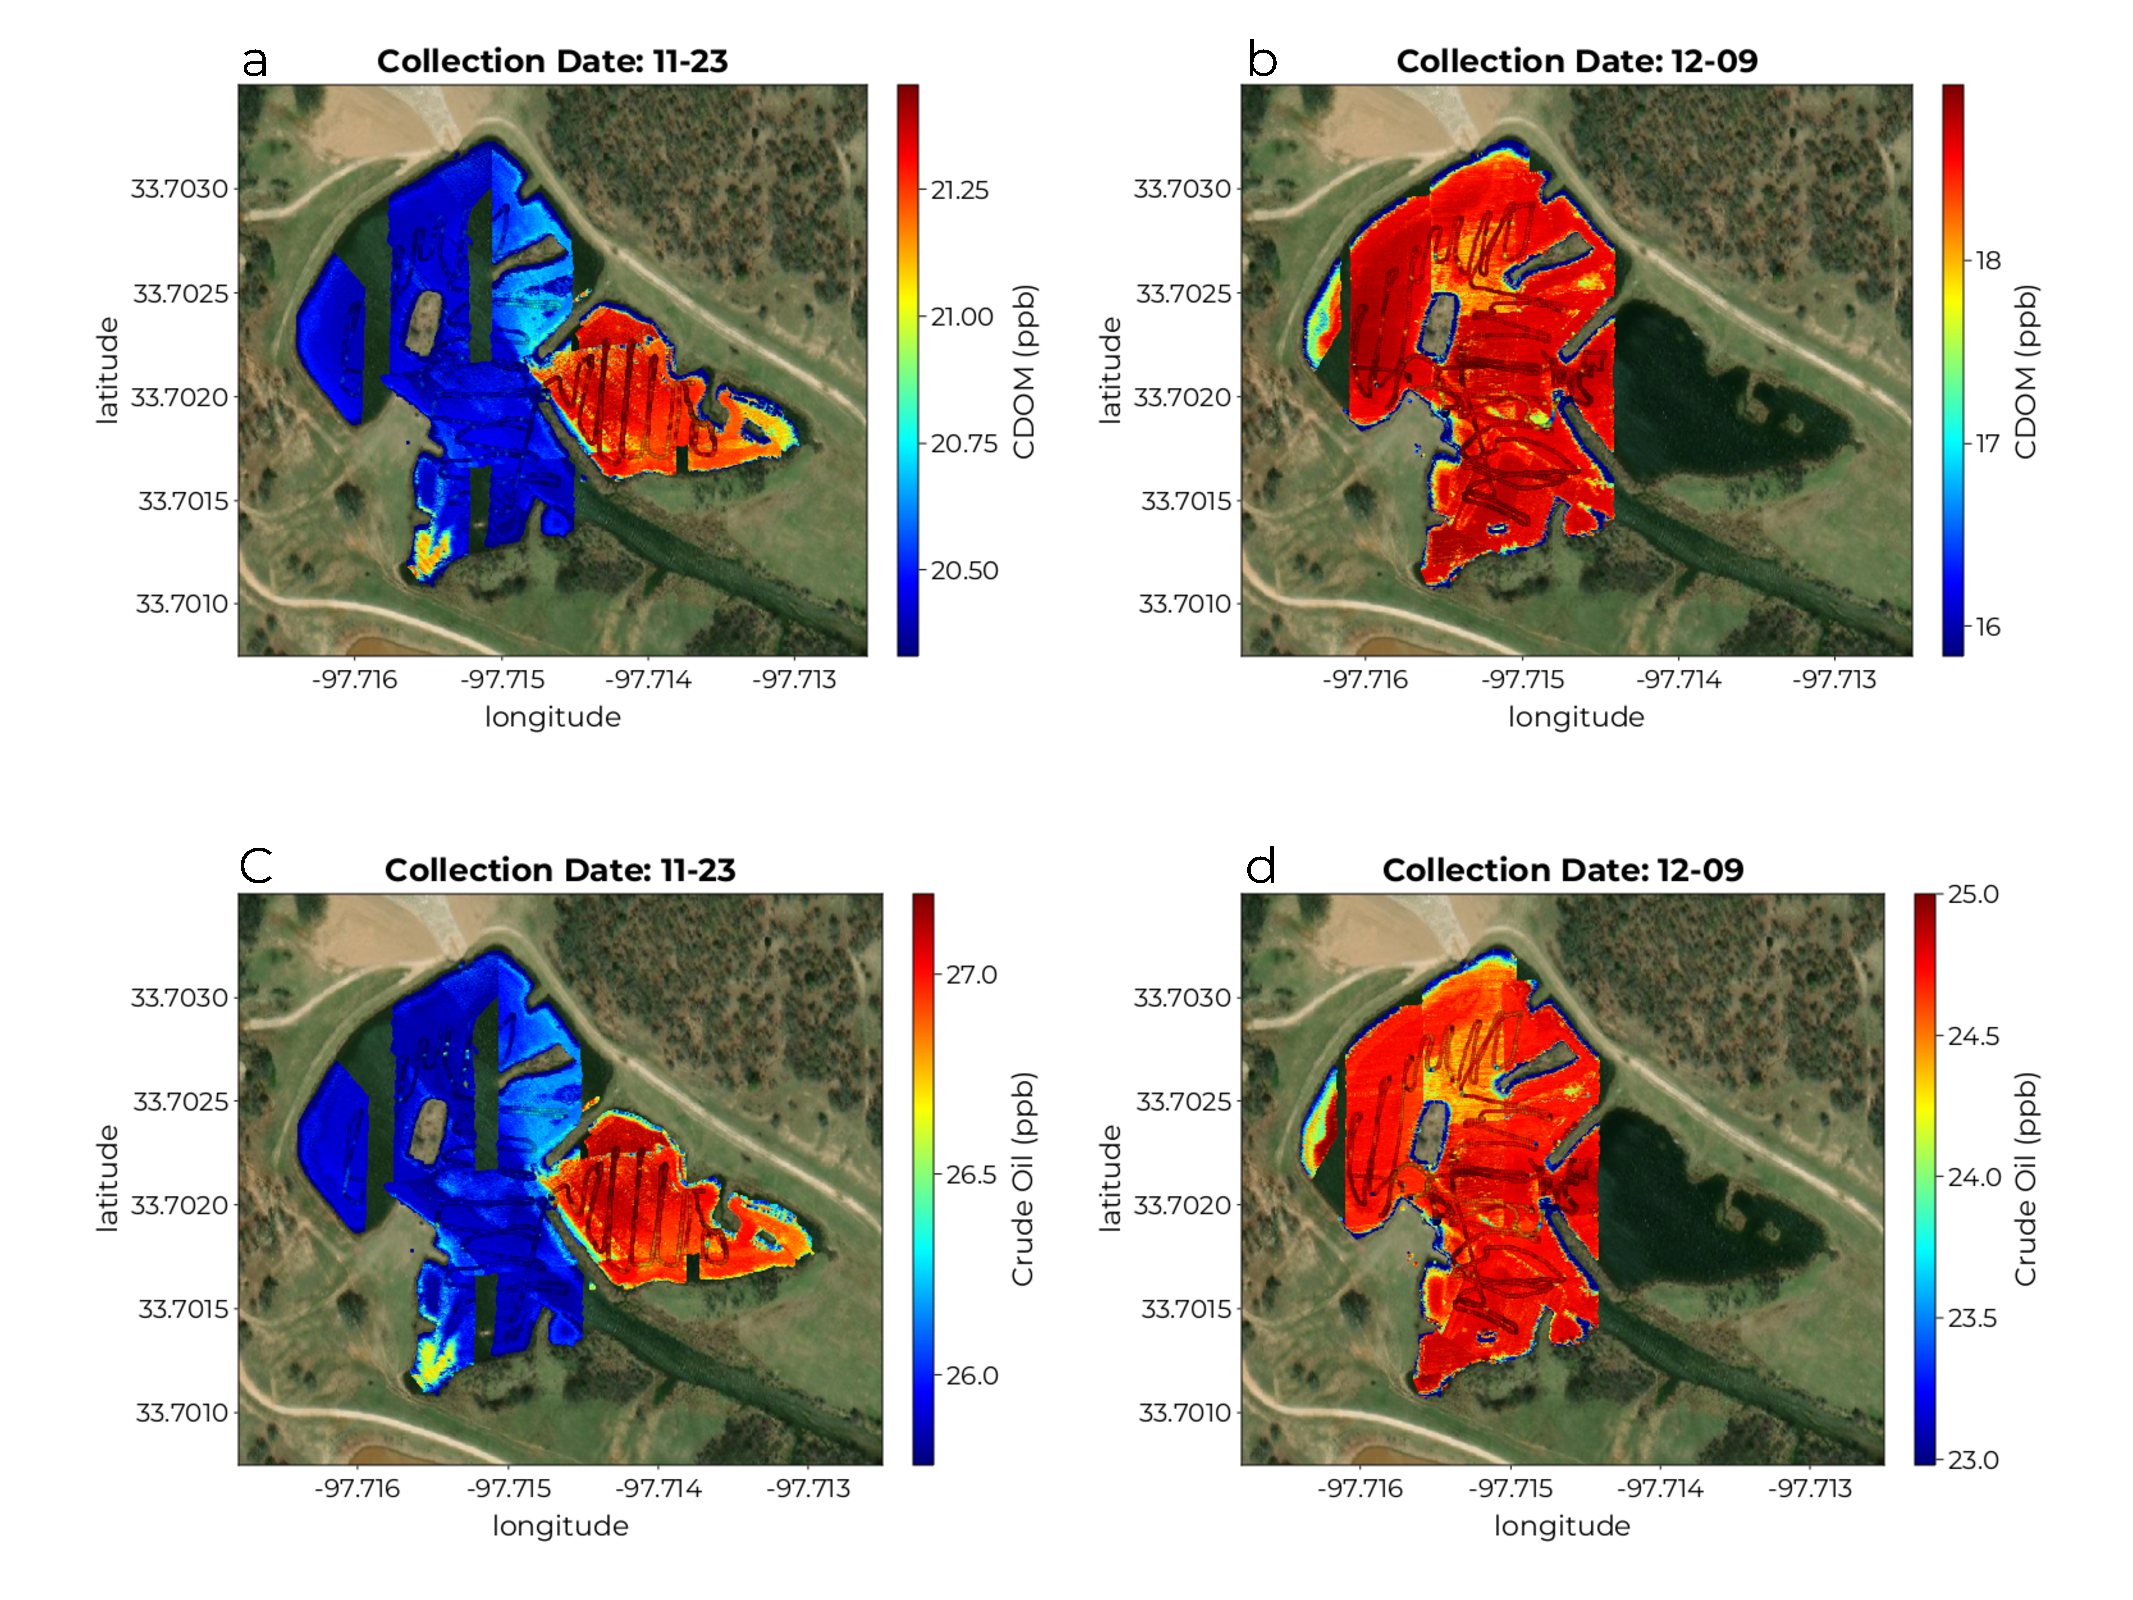
\includegraphics[width=18.0cm]{figures/results/map-combined.pdf}
%\end{adjustwidth}
%\caption{Maps generated by applying the ML model to hyperspectral data cubes. (\textbf{a}) The CDOM model applied to the 11-23 collection. (\textbf{b}) The CDOM model applied the the 12-09 collection. (\textbf{c}) the Crude Oil model applied to the 11-23 collection. (\textbf{d}) The Crude Oil model applied to the 12-09 collection. In each panel, boat data are overlaid as color-filled squares. We note that there is good agreement between estimated values at boat locations and the in situ reference measurements. \label{fig:maps}}
%\end{figure}  
\begin{figure}[H]

\vspace{-0.21in}
\hspace{-6pt}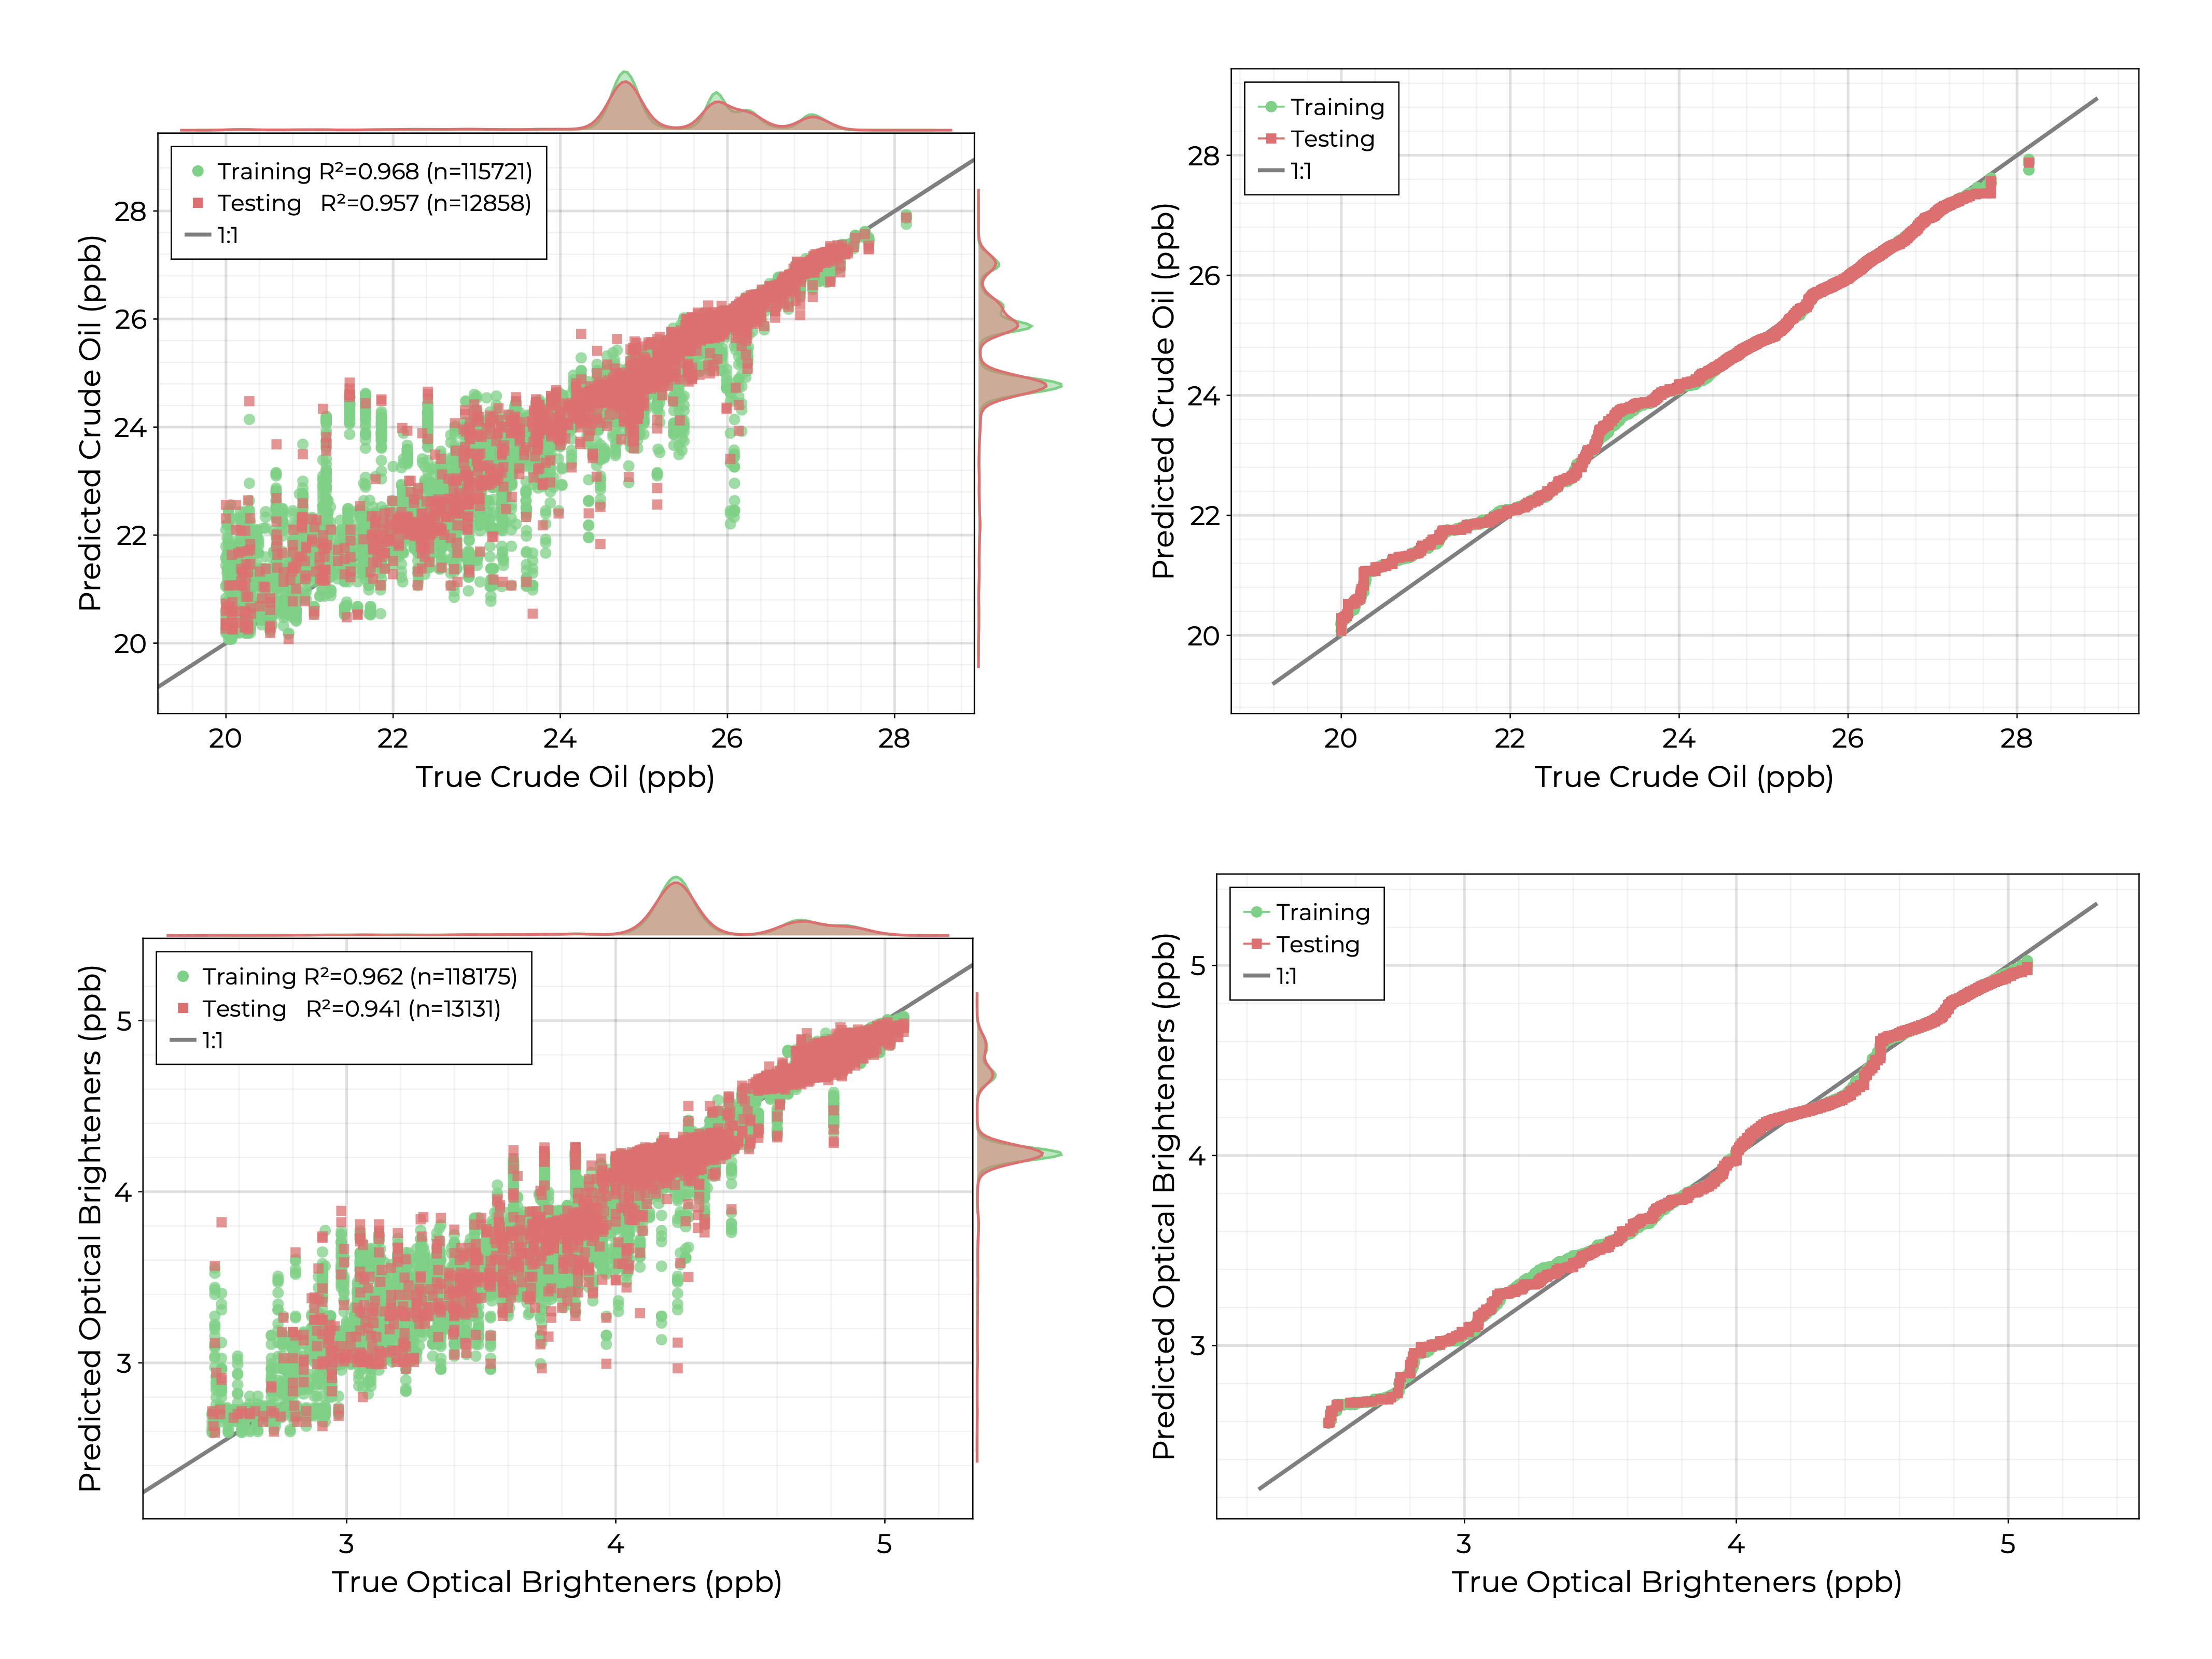
\includegraphics[width=\columnwidth]{figures/results/fits/chemical-fitres.png}
\vspace{-0.11in}
\caption{\hl{Scatter} %MDPI: Please use commas to separate thousands for numbers with five or more digits (not four digits) in the picture, e.g., "10000" should be "10,000".
 diagrams (\textbf{left}) and quantile--quantile plots (\textbf{right}) for the hyperparameter-optimized RFR models for the chemical variables measured by the USV.\label{fig:chemicals-fit}}
\end{figure}  

\vspace{-9pt}
\begin{figure}[H]
\vspace{-0.15in}
\hspace{-6pt}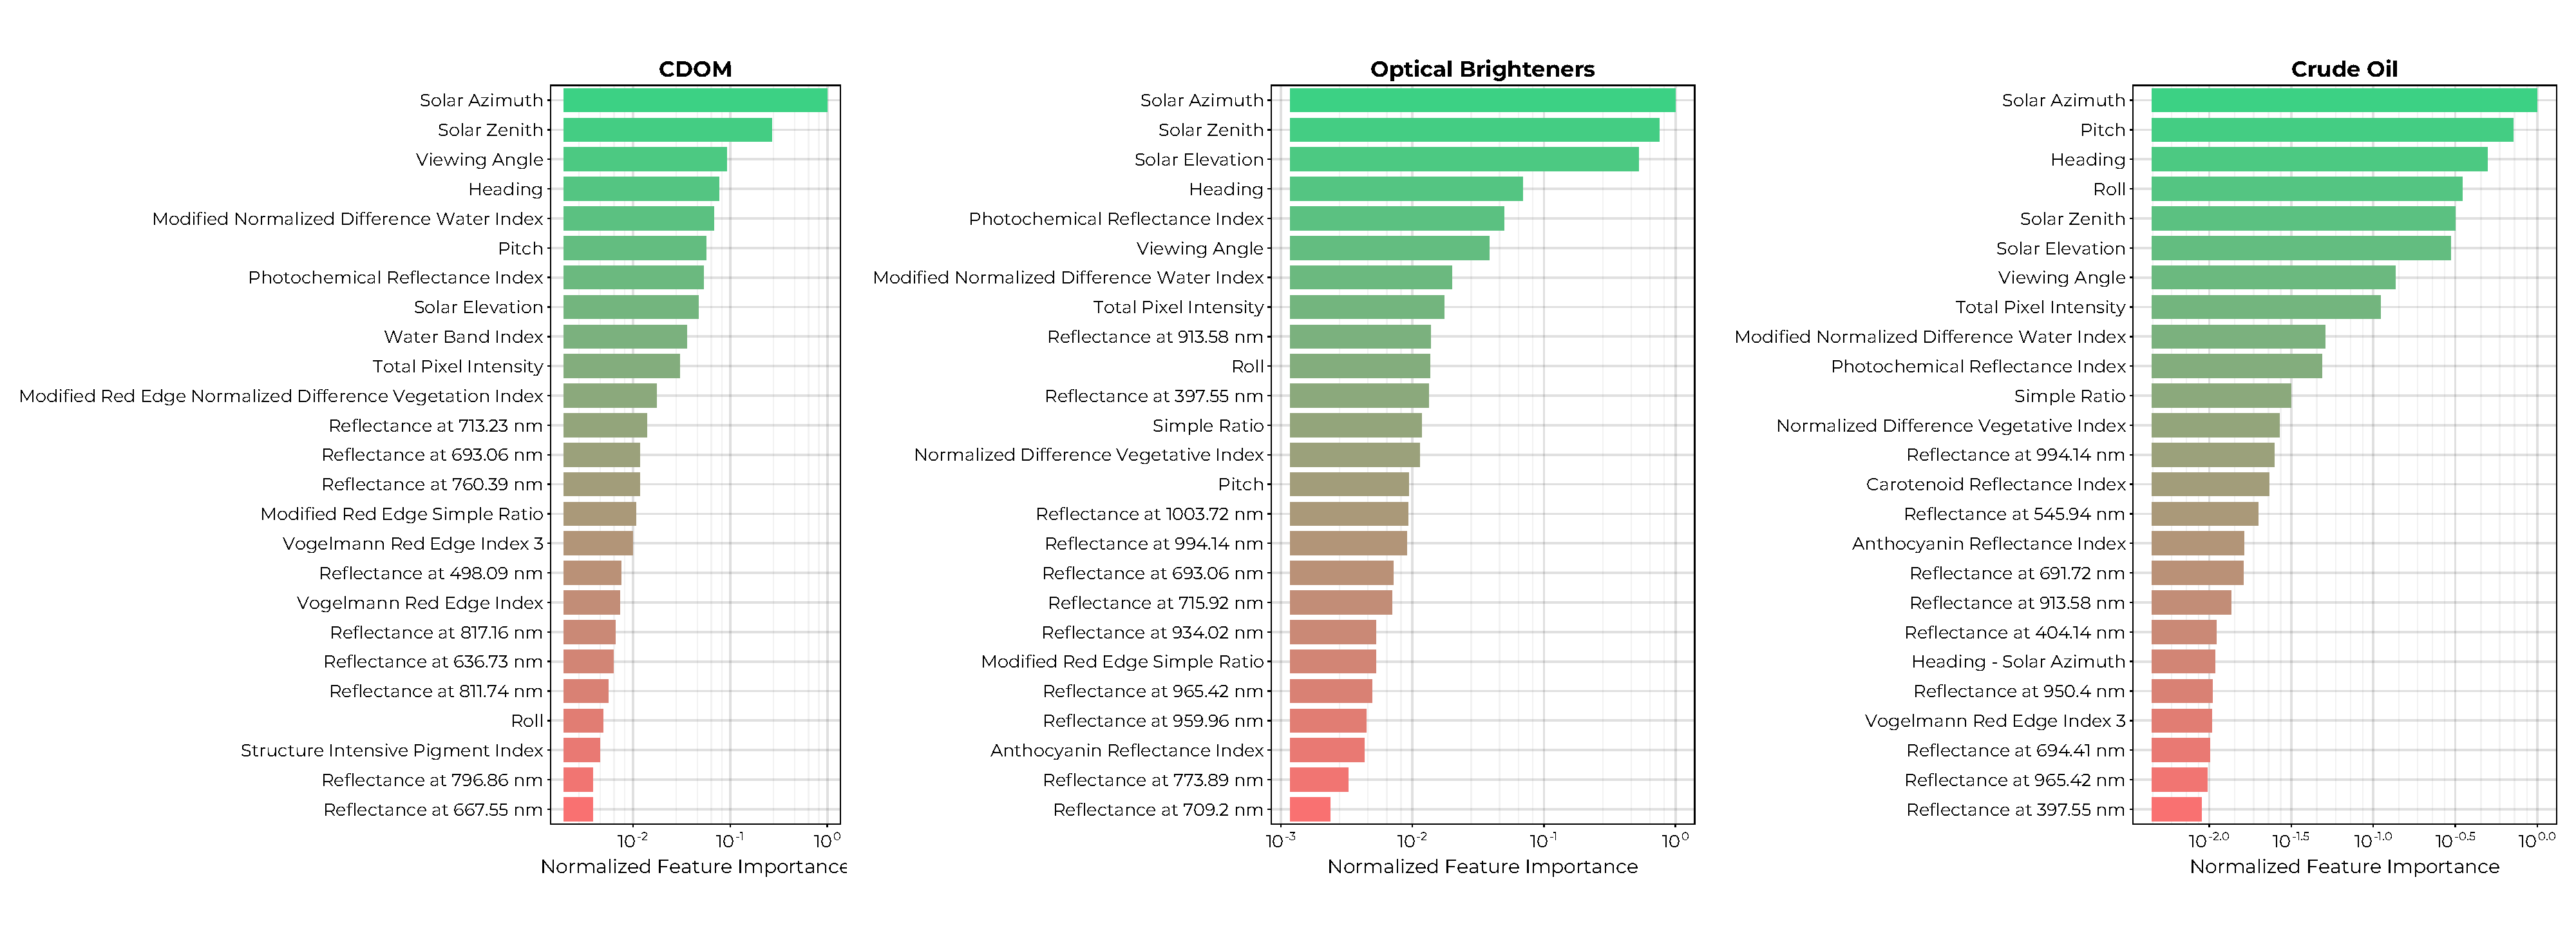
\includegraphics[width=\columnwidth]{figures/results/fits/chemical-ranking.pdf}
\vspace{-0.15in}
\caption{\hl{Ranked} %MDPI: Please change the hyphen (-) into a minus sign ($-$, "U+2212"). e.g., "-1" should be "$-$1".
 permutation importance for the top 25 features of the chemical models. The permutation importance measures the decrease in the model's $R^2$ value after replacing each feature in the prediction set with a random permutation of its values.\label{fig:chemicals-fi}}
\end{figure}  

\begin{figure}[H]

\vspace{-0.2in}
\hspace{-6pt}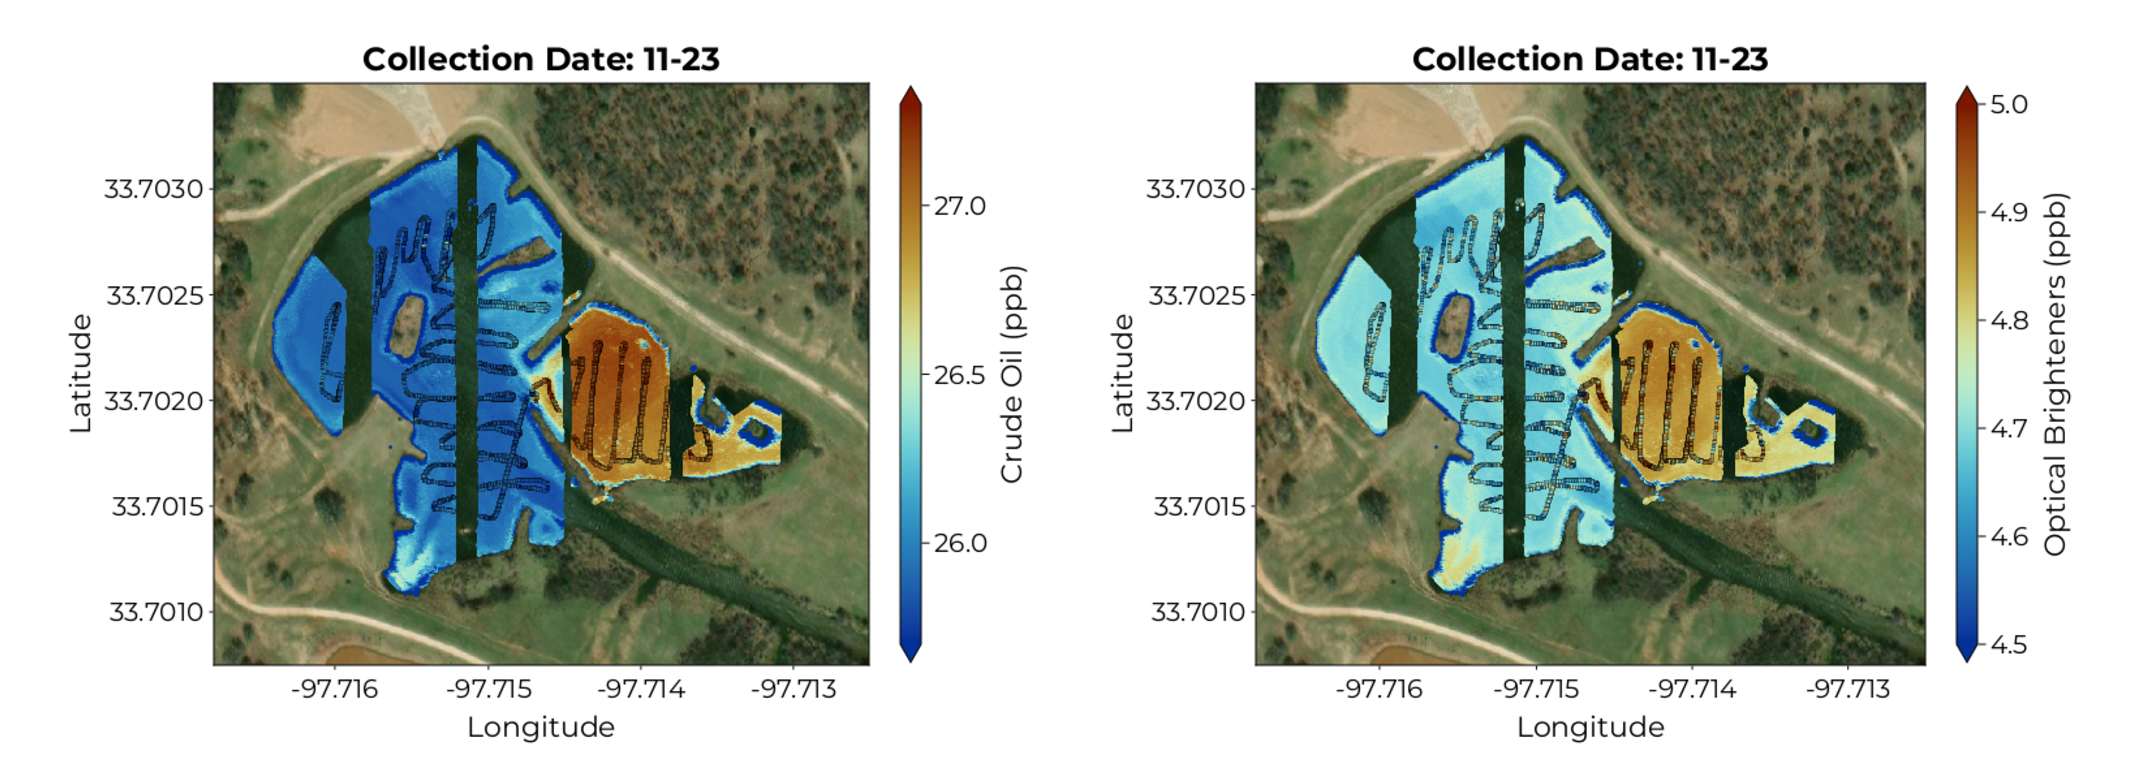
\includegraphics[width=\columnwidth]{figures/results/maps/chemical.pdf}
\vspace{-0.1in}
\caption{\hl{Maps} %MDPI: Please change the hyphen (-) into a minus sign ($-$, "U+2212"). e.g., "-1" should be "$-$1".
 generated by applying the trained chemical variable models to the hyperspectral data cubes collected on 23 November. Overlaid are color-filled squares showing the in situ reference data for the same collection period. The size of the squares is exaggerated for the visualization. We note that there is good agreement between the model predictions and reference data.\label{fig:map-chem}}
\end{figure} 

%%%%%%%%%%%%%%%%%%%%%%%%%%%%%%%%%%%%%%%%%%
\section{Discussion} \label{sec:discussion}

In recent years, much effort has been spent on the curation of comprehensive datasets combining water quality records with decades of satellite imagery to enable the development of new methods for retrieving water quality parameters. For example, Aurin et al. curated over 30 years of oceanographic field campaign data with associated coincident satellite imagery \cite{aurin2018remote}. Similarly, Ross et al. combined more than 600,000 records of dissolved organic carbon, chlorophyll-a and other water quality variables with historical Landsat reflectance data for the period 1984--2019 \cite{ross2019aquasat}. The sensing paradigm we have demonstrated here was able to rapidly collect comparable volumes of data within the span of just three observation periods. Therefore, despite the fact that individual UAV tracks cover far less spatial extent than remote sensing imagery, the ability to collect coordinated in situ measurements together with detailed hyperspectral images offers a significant improvement over these traditional approaches. With a coordinated robot team, one does not need to rely on infrequent satellite overpasses when planning data collection. Furthermore, the time offset between reference measurements and remote sensing is significantly reduced from days to minutes.

This study is not the first to employ UAVs equipped with multispectral or hyperspectral imagers for the purpose of assessing water composition and quality. Indeed there are many such examples focused on inferring optically active and inactive water quality parameters using band ratios and machine learning methods \cite{vogt2016near,lu2021retrieval, zhang2022selection}. The key advancement demonstrated by our robot team is the ability to combine UAV-borne hyperspectral imagers together with comprehensive, in situ sensing for a significant improvement in data volume. Purposefully coordinating USV sampling with the flight tracks of the UAV greatly accelerates data collection by removing the need to acquire individual samples for the calibration of water quality models. Additionally, the USV facilitates rapid validation of model predictions. When a trained model applied to collected hyperspectral imagery suggests elevated levels of a particular water quality parameter, the USV can quickly be provisioned to confirm these estimates with its reference instruments. 

In \cite{robotTeam1}, we introduced this paradigm. In this study, we have built on this approach in three new ways. First, we have demonstrated the ability to effectively combine observations from disparate collections by augmenting the machine learning models with sufficient features describing the illumination and viewing geometries. As Figure~\ref{fig:downwelling-hist} indicates, we observed variation in the total downwelling intensity between the images collected on the same day and between each separate collection period. These within-collection variations are due to a combination of the stability of the UAV (on which the upward facing downwelling irradiance spectrometer is mounted) together with the occasional interference of clouds. Moreover, the assumption that the water's surface can be treated as Lambertian is clearly violated when the water is not perfectly still. Despite the potential impact of these limitations on the quality of the resulting reflectance data cubes, the smoothness of the maps generated by our models suggests that we have provided sufficient context by including the relevant solar illumination and viewing angles as additional features in the final dataset.  This fact is reinforced by the position of these variables as the most important features for each of the estimated water quality variables. As long as we are primarily interested in these values and not the reflectances themselves, we are able to successfully account for these lighting effects when combining data from multiple collections.

The second contribution of this study is to explore the breadth of possible water quality and composition parameters that can be accurately mapped by hyperspectral imagery collected by the UAV. The results presented here confirm the ability of the robot team to predict optically active parameters including blue--green algae, chlorophyll-a, CDOM, crude oil, optical brighteners, turbidity, and temperature. Additionally, we are also able to infer the distributions of optically inactive variables including conductivity, pH, and ion concentrations. Other studies using multispectral and hyperspectral remote sensing imagery have also estimated optically inactive water quality parameters, with the ability to do so stemming from the relationship of these variables to optically active properties of the water \cite{vakili2020determination,guo2021machine,niu2021deep}. We note that in our investigation, the models trained for many of these variables outperformed their optically active counterparts. As the abundance of these variables is likely tied to the specific composition and content of the pond, it is unlikely that models trained for these optically inactive variables will generalize to other bodies of water. 

The third contribution of this work is the extension of our machine learning approach to enable uncertainty quantification through conformal prediction. For water quality risk assessment, the trustworthiness of model predictions is of equal or greater importance to the values themselves. However, robust uncertainty quantification has historically been challenging for many machine learning models, which behave like black boxes.
Conformal prediction is an attractive approach to enable model-agnostic uncertainty estimation and has recently seen adoption to remote sensing classification tasks such as land-type classification and object identification \cite{valle2023quantifying, zhu2024inductive}. In this setting, the goal is to produce predictive sets guaranteed to contain the correct class labels at a predetermined confidence level. Nevertheless, conformal prediction works equally well for regression tasks. By leveraging the large data volume collected by the robot team, we are able to simultaneously train predictive models and evaluate confidence intervals for their predictions. As the final column of Table~\ref{tab:fit-results} confirms, the empirical coverage on the holdout testing set provided by the inferred confidence intervals achieves the desired coverage to within 1\%. We chose to use a 90\% confidence interval for this study, but this can easily be adapted to suite the needs of a specific application if greater confidence is required. 

Despite the wealth of information provided by the increased resolution of hyperspectral images, their considerable size impedes their complete utilization in real-time applications. Often, much of the available spectral information is discarded in favor of indices like the NDVI, which can be quickly computed as images are captured \cite{horstrand2019uav}. Utilizing machine learning allows us to take advantage of the full spectrum captured by each pixel while simultaneously reducing the size of the final data product to single-band ``images'' of selected water quality variables. We note that training a reduced-feature model without further hyperparameter optimization takes roughly one minute per target variable of interest using the processing computer included on the UAV. This means that, in principle, training data can be collected by the USV, imagery can be acquired and processed by the UAV, coincident records can be selected, and the resulting dataset can be used to train machine learning models all while investigators are still in the field. Analyzing the maps produced by applying each trained model enables areas of interest to be readily pinpointed, as demonstrated by the identification of slightly elevated levels of %Please ensure meaning has been retained. 
crude oil, optical brighteners, and CDOM in the eastern alcove of the pond on 23 November. 

Finally, we note that the high spectral resolution of the UAV imagery together with the ability to collect precisely co-located reference measurements provides fertile ground for the development of new spectral indices targeted towards water quality variables. In this paper, we have shown that permutation importance ranking for trained machine learning models enables a straightforward interpretation of the relative values of each reflectance bin to the final model predictions. In future work, we plan to utilize this information to identify combinations of spectral bands that can be applied to remote sensing imagery captured by satellites equipped with hyperspectral imagers. The recently launched Environmental Mapping and Analysis Program (EnMAP) is one such example and includes over 91 spectral bands in the VNIR that overlap with those of our hyperspectral imager \cite{Storch2023TheEI}. 


%%%%%%%%%%%%%%%%%%%%%%%%%%%%%%%%%%%%%%%%%%
\section{Conclusions}

In this study, we address two key limitations of current remote sensing approaches to characterize water quality: namely, the limited spatial, spectral, and temporal resolution provided by existing satellite platforms and the lack of comprehensive in situ measurements needed to validate remote sensing data products. By equipping an autonomous USV with a suite of reference sensors, we rapidly collect significantly more data than existing approaches that rely on the collection of individual samples for lab analysis or are constrained to continuous sensing at fixed sites. Utilizing an autonomous UAV equipped with a hyperspectral imager in tandem with the USV allows us to quickly generate aligned datasets that are used to train machine learning models mapping measured reflectance spectra to the desired water quality variables. By virtue of this increased data volume, we are able to simultaneously estimate the uncertainty of our models by using conformal prediction. Finally, the hyperspectral data cube processing workflow employed onboard the UAV makes it possible to deploy these trained models to swiftly generate maps of the target variables across bodies of water. The rapid turnaround time from data collection to model deployment is critical for real-time water quality evaluation and risk assessment. 



%%%%%%%%%%%%%%%%%%%%%%%%%%%%%%%%%%%%%%%%%%
\vspace{6pt} 
%%%%%%%%%%%%%%%%%%%%%%%%%%%%%%%%%%%%%%%%%%
%% optional
\supplementary{The following supporting information can be downloaded at:  \linksupplementary{s1}, \hl{Table S1:} %MDPI: please provide an independent file to indicate supplementary materials.
 Hyperspectral reflectance indices.}

% Only for journal Methods and Protocols:
% If you wish to submit a video article, please do so with any other supplementary material.
% \supplementary{The following supporting information can be downloaded at: \linksupplementary{s1}, Figure S1: title; Table S1: title; Video S1: title. A supporting video article is available at doi: link.}

% Only for journal Hardware:
% If you wish to submit a video article, please do so with any other supplementary material.
% \supplementary{The following supporting information can be downloaded at: \linksupplementary{s1}, Figure S1: title; Table S1: title; Video S1: title.\vspace{6pt}\\
%\begin{tabularx}{\textwidth}{lll}
%\toprule
%\textbf{Name} & \textbf{Type} & \textbf{Description} \\
%\midrule
%S1 & Python script (.py) & Script of python source code used in XX \\
%S2 & Text (.txt) & Script of modelling code used to make Figure X \\
%S3 & Text (.txt) & Raw data from experiment X \\
%S4 & Video (.mp4) & Video demonstrating the hardware in use \\
%... & ... & ... \\
%\bottomrule
%\end{tabularx}
%}

%%%%%%%%%%%%%%%%%%%%%%%%%%%%%%%%%%%%%%%%%%
\authorcontributions{Conceptualization, D.J.L.; methodology, \hl{J.W.} %MDPI: We changed all J.L.W. into J.W. Please confirm.
 and D.J.L; software, J.W.; field deployment and preparation, J.W., A.A., L.O.H.W., S.T., B.F., P.M.H.D., M.I., M.L., D.S., and D.J.L.; validation, J.W.; formal analysis, J.W.; investigation J.W.; resources, D.J.L.; data curation, J.W., A.A., L.O.H.W., and D.J.L; writing---original draft preparation, J.W.; writing---review and editing, J.W. and D.J.L.; visualization, J.W.; supervision, D.J.L.; project administration, D.J.L.; funding acquisition, D.J.L. All authors have read and agreed to the published version of the manuscript.
}


\newpage
\funding{This research was funded by the following grants: the Texas National Security Network Excellence Fund award for Environmental Sensing Security Sentinels; the SOFWERX award for Machine Learning for Robotic Teams %Please ensure meaning has been retained. 
	and NSF Award OAC-2115094; support from the University of Texas at Dallas Office of Sponsored Programs, Dean of Natural Sciences and Mathematics, and Chair of the Physics Department is gratefully acknowledged; TRECIS CC* Cyberteam (NSF \#2019135); NSF OAC-2115094 Award; and EPA P3 grant number 84057001-0.
}

\institutionalreview{Not applicable.}

\informedconsent{Not applicable.}

\dataavailability{The raw data supporting the conclusions of this article will be made available by the authors on request.} 

% Only for journal Nursing Reports
%\publicinvolvement{Please describe how the public (patients, consumers, carers) were involved in the research. Consider reporting against the GRIPP2 (Guidance for Reporting Involvement of Patients and the Public) checklist. If the public were not involved in any aspect of the research add: ``No public involvement in any aspect of this research''.}

% Only for journal Nursing Reports
%\guidelinesstandards{Please add a statement indicating which reporting guideline was used when drafting the report. For example, ``This manuscript was drafted against the XXX (the full name of reporting guidelines and citation) for XXX (type of research) research''. A complete list of reporting guidelines can be accessed via the equator network: \url{https://www.equator-network.org/}.}

\acknowledgments{Don MacLaughlin, Scotty MacLaughlin, and the city of Plano, TX, are gratefully acknowledged for allowing us to deploy the autonomous robot team on their property.  Christopher Simmons is gratefully acknowledged for his computational support. We thank  Antonio Mannino for his advice with regard to selecting the robotic boat's sensing suite. Annette Rogers is gratefully acknowledged for supporting the arrangement of insurance coverage. Steven Lyles is gratefully acknowledged for supporting the arrangement of a secure place for the robot team. The authors acknowledge the OIT-Cyberinfrastructure Research Computing group at the University of Texas at Dallas and the TRECIS CC* Cyberteam (NSF \#2019135) for providing HPC resources that contributed to this research; the authors also acknowledge their receipt of the %Please ensure meaning has been retained. 
	NSF OAC-2115094 Award and EPA P3 grant number 84057001-0.}

\conflictsofinterest{The authors declare no conflicts of interest.}

%%%%%%%%%%%%%%%%%%%%%%%%%%%%%%%%%%%%%%%%%%
%% Optional

%% Only for journal Encyclopedia
%\entrylink{The Link to this entry published on the encyclopedia platform.}

\abbreviations{Abbreviations}{
The following abbreviations are used in this manuscript:\\

\noindent 
\begin{tabular}{@{}ll}
GPS & Global Positioning System \\ 
INS & Inertial Navigation System \\
UTM & Universal Transverse Mercator \\
UV & Ultraviolet \\
ML & Machine Learning \\
USV & Uncrewed Surface Vessel \\
UAV & Unmanned Aerial Vehicle \\
CDOM & Colored Dissolved Organic Matter \\
CO & Crude Oil \\ 
OB & Optical Brighteners \\
FNU & Formazin Nephelometric Unit \\
RFR & Random Forest Regressor \\
MLJ & Machine Learning framework for Julia \\
RMSE & Root Mean Square Error \\ 
MAE & Mean Absolute Error \\
RENDVI & Red-Edge Normalized Difference Vegetation Index
\end{tabular}
}

%%%%%%%%%%%%%%%%%%%%%%%%%%%%%%%%%%%%%%%%%%
%% Optional
\appendixtitles{no} % Leave argument "no" if all appendix headings stay EMPTY (then no dot is printed after "Appendix A"). If the appendix sections contain a heading then change the argument to "yes".
\appendixstart
\appendix
\section[\appendixname~\thesection]{}\label{Model Hyperparameters}
%% \subsection[\appendixname~\thesubsection]{}

\vspace{-6pt}
\begin{table}[H] 
\caption{Final hyperparameter values for each target model. The number of trees and the sampling ratio were optimized using a random search. The maximum tree depth was fixed to 20 to limit overfitting and to control the size of the final model. The number of sub-features was set to the square root of the total number of features, and the minimum samples per leaf and minimum samples per split were left to their default values. \label{tab:hyperparameters}}
\newcolumntype{C}{>{\centering\arraybackslash}X}
\begin{tabularx}{\textwidth}{CCCCCCC}
\toprule
\textbf{Target}	& \textbf{Number of Trees}	& \textbf{Sampling Ratio} & \textbf{Maximum Tree Depth} & \textbf{Number of Sub-Features} & \textbf{Minimum Samples per Leaf} & \textbf{Minimum Samples per Split}\\
\midrule
Temperature & 153 & 0.979 & 20 & 5 & 1 & 2 \\
Conductivity & 154 & 0.992 & 20 & 5 & 1 & 2\\
pH & 103 & 0.972 & 20 & 5 & 1 & 2\\
Turbidity & 158 & 0.998 & 20 & 5 & 1 & 2\\

\bottomrule
\end{tabularx}
%\end{adjustwidth}
\end{table}

\begin{table}[H]\ContinuedFloat
\small
\caption{\textit{Cont.}}

\newcolumntype{C}{>{\centering\arraybackslash}X}
\begin{tabularx}{\textwidth}{CCCCCCC}
\toprule
\textbf{Target}	& \textbf{Number of Trees}	& \textbf{Sampling Ratio} & \textbf{Maximum Tree Depth} & \textbf{Number of Sub-Features} & \textbf{Minimum Samples per Leaf} & \textbf{Minimum Samples per Split}\\
\midrule
$\mathrm{Ca}^{2+}$ & 172 & 0.984 & 20 & 5 & 1 & 2\\
$\mathrm{Cl^-}$ & 110 & 0.999 & 20 & 5 & 1 & 2\\
$\mathrm{Na^+}$ & 103 & 0.972 & 20 & 5 & 1 & 2\\
%\begin{adjustwidth}{-\extralength}{0cm}%\centering
%Blue-Green Algae (Phycoerythrin) & 153 & 0.979 & 20 & 5 & 1 & 2\\
Phycoerythrin & 158 & 0.998 & 20 & 5 & 1 & 2\\
CDOM & 157 & 0.982 & 20 & 5 & 1 & 2\\
Chlorophyll-a & 158 & 0.998 & 20 & 5 & 1 & 2\\
%Blue-Green Algae (Phycocyanin) & 153 & 0.979 & 20 & 5 & 1 & 2\\
Phycocyanin & 142 & 0.995 & 20 & 5 & 1 & 2\\
Crude Oil & 154 & 0.992 & 20 & 5 & 1 & 2\\
Optical Brighteners & 157 & 0.982 & 20 & 5 & 1 & 2\\
\bottomrule
\end{tabularx}
\end{table}


%%%%%%%%%%%%%%%%%%%%%%%%%%%%%%%%%%%%%%%%%%
\begin{adjustwidth}{-\extralength}{0cm}
%\printendnotes[custom] % Un-comment to print a list of endnotes

\reftitle{References}

% Please provide either the correct journal abbreviation (e.g. according to the “List of Title Word Abbreviations” http://www.issn.org/services/online-services/access-to-the-ltwa/) or the full name of the journal.
% Citations and References in Supplementary files are permitted provided that they also appear in the reference list here. 

%=====================================
% References, variant A: external bibliography
%=====================================

\begin{thebibliography}{999}

\bibitem[Melesse et~al.(2007)Melesse, Weng, Thenkabail, and
  Senay]{melesse2007remote}
Melesse, A.M.; Weng, Q.; Thenkabail, P.S.; Senay, G.B.
\newblock Remote sensing sensors and applications in environmental resources
  mapping and modelling.
\newblock {\em Sensors} {\bf 2007}, {\em 7},~3209--3241.

\bibitem[Joyce et~al.(2009)Joyce, Belliss, Samsonov, McNeill, and
  Glassey]{joyce2009review}
Joyce, K.E.; Belliss, S.E.; Samsonov, S.V.; McNeill, S.J.; Glassey, P.J.
\newblock A review of the status of satellite remote sensing and image
  processing techniques for mapping natural hazards and disasters.
\newblock {\em Prog. Phys. Geogr.} {\bf 2009}, {\em 33},~183--207.

\bibitem[Aurin et~al.(2018)Aurin, Mannino, and Lary]{aurin2018remote}
Aurin, D.; Mannino, A.; Lary, D.J.
\newblock Remote sensing of CDOM, CDOM spectral slope, and dissolved organic
  carbon in the global ocean.
\newblock {\em Appl. Sci.} {\bf 2018}, {\em 8},~2687.

\bibitem[Ross et~al.(2019)Ross, Topp, Appling, Yang, Kuhn, Butman, Simard, and
  Pavelsky]{ross2019aquasat}
Ross, M.R.; Topp, S.N.; Appling, A.P.; Yang, X.; Kuhn, C.; Butman, D.; Simard,
  M.; Pavelsky, T.M.
\newblock AquaSat: A data set to enable remote sensing of water quality for
  inland waters.
\newblock {\em Water Resour. Res.} {\bf 2019}, {\em 55},~10012--10025.

\bibitem[Fingas and Brown(2017)]{fingas2017review}
Fingas, M.; Brown, C.E.
\newblock A review of oil spill remote sensing.
\newblock {\em Sensors} {\bf 2017}, {\em 18},~91.

\bibitem[Koponen et~al.(2007)Koponen, Attila, Pulliainen, Kallio,
  Pyh{\"a}lahti, Lindfors, Rasmus, and Hallikainen]{remote-sensing-finland}
Koponen, S.; Attila, J.; Pulliainen, J.; Kallio, K.; Pyh{\"a}lahti, T.;
  Lindfors, A.; Rasmus, K.; Hallikainen, M.
\newblock A case study of airborne and satellite remote sensing of a spring
  bloom event in the Gulf of Finland.
\newblock {\em Cont. Shelf Res.} {\bf 2007}, {\em 27},~228--244.

\bibitem[Bonansea et~al.(2015)Bonansea, Rodriguez, Pinotti, and
  Ferrero]{bonansea2015using}
Bonansea, M.; Rodriguez, M.C.; Pinotti, L.; Ferrero, S.
\newblock Using multi-temporal Landsat imagery and linear mixed models for
  assessing water quality parameters in R{\'\i}o Tercero reservoir (Argentina).
\newblock {\em Remote Sens. Environ.} {\bf 2015}, {\em 158},~28--41.

\bibitem[Absalon et~al.(2023)Absalon, Matysik, Wo{\'z}nica, and
  Janczewska]{absalon2023detection}
Absalon, D.; Matysik, M.; Wo{\'z}nica, A.; Janczewska, N.
\newblock Detection of changes in the hydrobiological parameters of the Oder
  River during the ecological disaster in July 2022 based on multi-parameter
  probe tests and remote sensing methods.
\newblock {\em Ecol. Indic.} {\bf 2023}, {\em 148},~110103.

\bibitem[Lary(2010)]{lary2010artificial}
Lary, D.J.
\newblock Artificial intelligence in geoscience and remote sensing. In {\em
  Geoscience and Remote Sensing New Achievements}; \hl{IntechOpen:} %MDPI: Please add the location of the publisher (City and Country).
  2010.

\bibitem[Peterson et~al.(2020)Peterson, Sagan, and Sloan]{peterson2020deep}
Peterson, K.T.; Sagan, V.; Sloan, J.J.
\newblock Deep learning-based water quality estimation and anomaly detection
  using Landsat-8/Sentinel-2 virtual constellation and cloud computing.
\newblock {\em GIScience  Remote Sens.} {\bf 2020}, {\em 57},~510--525.

\bibitem[Belgiu and Dr{\u{a}}gu{\c{t}}(2016)]{belgiu2016random}
Belgiu, M.; Dr{\u{a}}gu{\c{t}}, L.
\newblock Random forest in remote sensing: A review of applications and future
  directions.
\newblock {\em ISPRS J. Photogramm. Remote Sens.} {\bf 2016},
  {\em 114},~24--31.

\bibitem[Sagan et~al.(2020)Sagan, Peterson, Maimaitijiang, Sidike, Sloan,
  Greeling, Maalouf, and Adams]{sagan2020monitoring}
Sagan, V.; Peterson, K.T.; Maimaitijiang, M.; Sidike, P.; Sloan, J.; Greeling,
  B.A.; Maalouf, S.; Adams, C.
\newblock Monitoring inland water quality using remote sensing: Potential and
  limitations of spectral indices, bio-optical simulations, machine learning,
  and cloud computing.
\newblock {\em Earth-Sci. Rev.} {\bf 2020}, {\em 205},~103187.

\bibitem[Hruska et~al.(2012)Hruska, Mitchell, Anderson, and
  Glenn]{hruska2012radiometric}
Hruska, R.; Mitchell, J.; Anderson, M.; Glenn, N.F.
\newblock Radiometric and geometric analysis of hyperspectral imagery acquired
  from an unmanned aerial vehicle.
\newblock {\em Remote Sens.} {\bf 2012}, {\em 4},~2736--2752.

\bibitem[Ad{\~a}o et~al.(2017)Ad{\~a}o, Hru{\v{s}}ka, P{\'a}dua, Bessa, Peres,
  Morais, and Sousa]{adao2017hyperspectral}
Ad{\~a}o, T.; Hru{\v{s}}ka, J.; P{\'a}dua, L.; Bessa, J.; Peres, E.; Morais,
  R.; Sousa, J.J.
\newblock Hyperspectral imaging: A review on UAV-based sensors, data processing
  and applications for agriculture and forestry.
\newblock {\em Remote Sens.} {\bf 2017}, {\em 9},~1110.

\bibitem[Banerjee et~al.(2020)Banerjee, Raval, and Cullen]{banerjee2020uav}
Banerjee, B.P.; Raval, S.; Cullen, P.
\newblock UAV-hyperspectral imaging of spectrally complex environments.
\newblock {\em Int. J. Remote Sens.} {\bf 2020}, {\em
  41},~4136--4159.

\bibitem[P{\'a}dua et~al.(2017)P{\'a}dua, Vanko, Hru{\v{s}}ka, Ad{\~a}o, Sousa,
  Peres, and Morais]{padua2017uas}
P{\'a}dua, L.; Vanko, J.; Hru{\v{s}}ka, J.; Ad{\~a}o, T.; Sousa, J.J.; Peres,
  E.; Morais, R.
\newblock UAS, sensors, and data processing in agroforestry: A review towards
  practical applications.
\newblock {\em Int. J.  Remote Sens.} {\bf 2017}, {\em
  38},~2349--2391.

\bibitem[Arroyo-Mora et~al.(2019)Arroyo-Mora, Kalacska, Inamdar, Soffer,
  Lucanus, Gorman, Naprstek, Schaaf, Ifimov, Elmer,
  et~al.]{arroyo2019implementation}
Arroyo-Mora, J.P.; Kalacska, M.; Inamdar, D.; Soffer, R.; Lucanus, O.; Gorman,
  J.; Naprstek, T.; Schaaf, E.S.; Ifimov, G.; Elmer, K.;  et~al.
\newblock Implementation of a UAV--hyperspectral pushbroom imager for
  ecological monitoring.
\newblock {\em Drones} {\bf 2019}, {\em 3},~12.

\bibitem[Kurihara et~al.(2020)Kurihara, Ishida, and
  Takahashi]{kurihara2020unmanned}
Kurihara, J.; Ishida, T.; Takahashi, Y.
\newblock Unmanned Aerial Vehicle (UAV)-based hyperspectral imaging system for
  precision agriculture and forest management.
\newblock In {\em Unmanned Aerial Vehicle: Applications in Agriculture and
  Environment}; \hl{2020} %MDPI: Please add the name of the publisher and their location.
; pp. 25--38.

\bibitem[Ehmann et~al.(2019)Ehmann, Kelleher, and Condon]{ehmann2019monitoring}
Ehmann, K.; Kelleher, C.; Condon, L.E.
\newblock Monitoring turbidity from above: Deploying small unoccupied aerial
  vehicles to image in-stream turbidity.
\newblock {\em Hydrol. Process.} {\bf 2019}, {\em 33},~1013--1021.

\bibitem[Lu et~al.(2021)Lu, Si, Wei, Li, Xia, Ye, and Xia]{lu2021retrieval}
Lu, Q.; Si, W.; Wei, L.; Li, Z.; Xia, Z.; Ye, S.; Xia, Y.
\newblock Retrieval of water quality from UAV-borne hyperspectral imagery: A
  comparative study of machine learning algorithms.
\newblock {\em Remote Sens.} {\bf 2021}, {\em 13},~3928.

\bibitem[Zhang et~al.(2022)Zhang, Zeng, and He]{zhang2022selection}
Zhang, D.; Zeng, S.; He, W.
\newblock Selection and Quantification of Best Water Quality Indicators Using
  UAV-Mounted Hyperspectral Data: A Case Focusing on a Local River Network in
  Suzhou City, China.
\newblock {\em Sustainability} {\bf 2022}, {\em 14},~16226.

\bibitem[Lary et~al.(2021)Lary, Schaefer, Waczak, Aker, Barbosa, Wijeratne,
  Talebi, Fernando, Sadler, Lary, and Lary]{robotTeam1}
Lary, D.J.; Schaefer, D.; Waczak, J.; Aker, A.; Barbosa, A.; Wijeratne, L.O.H.;
  Talebi, S.; Fernando, B.; Sadler, J.Z.; Lary, T.;  et~al.
\newblock Autonomous Learning of New Environments with a Robotic Team Employing
  Hyper-Spectral Remote Sensing, Comprehensive In-Situ Sensing and Machine
  Learning.
\newblock {\em Sensors} {\bf 2021}, {\em 21}, 2240.

\bibitem[Meier(2010)]{qgroundcontrol}
Meier, L.
\newblock QGroundControl.
\newblock  MAVLink Micro Air Vehicle Communication Protocol. 2010. Available
  online: \url{http://qgroundcontrol. org/mavlink/start} (accessed on 30 January
  2019).

\bibitem[De~Marco et~al.(2007)De~Marco, Clarke, and Pejcic]{de2007ion}
De~Marco, R.; Clarke, G.; Pejcic, B.
\newblock Ion-selective electrode potentiometry in environmental analysis.
\newblock {\em Electroanal. An Int. J. Devoted Fundam. Pract. Asp. Electroanal.} {\bf 2007}, {\em 19},~1987--2001.

\bibitem[Trees et~al.(2002)Trees, Bidigare, Karl, Van~Heukelem, and
  Dore]{trees2002fluorometric}
Trees, C.C.; Bidigare, R.R.; Karl, D.M.; Van~Heukelem, L.; Dore, J.
\newblock Fluorometric chlorophyll a: Sampling, laboratory methods, and data
  analysis protocols.
\newblock In \emph{Ocean Optics Protocols for Satellite Ocean Color Sensor
  Validation, NASA/TM-2002-210004/Rev3-Vol2};  Mueller, J.L., Fargion, G.S., Eds.; NASA Goddard Space Flight Center: Greenbelt, MD, USA, {2002}; pp. 269--283.

\bibitem[Tillman(2017)]{tillman2017evaluation}
Tillman, E.F.
\newblock \emph{Evaluation of the Eureka Manta2 Water-Quality Multiprobe Sonde};
\newblock Technical report; \hl{US Geological Survey:} %MDPI: Please add the location of the publisher (City and Country).
  2017.

\bibitem[Brient et~al.(2008)Brient, Lengronne, Bertrand, Rolland, Sipel,
  Steinmann, Baudin, Legeas, Rouzic, and Bormans]{Brient2008APP}
Brient, L.; Lengronne, M.; Bertrand, E.; Rolland, D.C.; Sipel, A.; Steinmann,
  D.; Baudin, I.; Legeas, M.; Rouzic, B.L.; Bormans, M.
\newblock A phycocyanin probe as a tool for monitoring cyanobacteria in
  freshwater bodies.
\newblock {\em J. Environ. Monit. JEM} {\bf 2008}, {\em 10},~248--255.

\bibitem[Boyer et~al.(2009)Boyer, Kelble, Ortner, and
  Rudnick]{boyer2009phytoplankton}
Boyer, J.N.; Kelble, C.R.; Ortner, P.B.; Rudnick, D.T.
\newblock Phytoplankton bloom status: Chlorophyll a biomass as an indicator of
  water quality condition in the southern estuaries of Florida, USA.
\newblock {\em Ecol. Indic.} {\bf 2009}, {\em 9},~S56--S67.

\bibitem[Brown and Fingas(2003)]{brown2003review}
Brown, C.E.; Fingas, M.F.
\newblock Review of the development of laser fluorosensors for oil spill
  application.
\newblock {\em Mar. Pollut. Bull.} {\bf 2003}, {\em 47},~477--484.

\bibitem[Cao et~al.(2009)Cao, Griffith, and Weisberg]{cao2009evaluation}
Cao, Y.; Griffith, J.F.; Weisberg, S.B.
\newblock Evaluation of optical brightener photodecay characteristics for
  detection of human fecal contamination.
\newblock {\em Water Res.} {\bf 2009}, {\em 43},~2273--2279.

\bibitem[Piper(1944)]{piper1944graphic}
Piper, A.M.
\newblock A graphic procedure in the geochemical interpretation of
  water-analyses.
\newblock {\em Eos Trans. Am. Geophys. Union} {\bf 1944}, {\em
  25},~914--928.

\bibitem[Dordoni et~al.(2023)Dordoni, Zappal{\`a}, and
  Barth]{dordoni2023preliminary}
Dordoni, M.; Zappal{\`a}, P.; Barth, J.A.
\newblock A preliminary global hydrochemical comparison of lakes and
  reservoirs.
\newblock {\em Front. Water} {\bf 2023}, {\em 5},~1084050.

\bibitem[Pace et~al.(2012)Pace, Reche, Cole, Fern{\'a}ndez-Barbero, Mazuecos,
  and Prairie]{pace2012ph}
Pace, M.L.; Reche, I.; Cole, J.J.; Fern{\'a}ndez-Barbero, A.; Mazuecos, I.P.;
  Prairie, Y.T.
\newblock pH change induces shifts in the size and light absorption of
  dissolved organic matter.
\newblock {\em Biogeochemistry} {\bf 2012}, {\em 108},~109--118.

\bibitem[Ruddick et~al.(2019)Ruddick, Voss, Banks, Boss, Castagna, Frouin,
  Hieronymi, Jamet, Johnson, Kuusk, et~al.]{reflectance-conversion}
Ruddick, K.G.; Voss, K.; Banks, A.C.; Boss, E.; Castagna, A.; Frouin, R.;
  Hieronymi, M.; Jamet, C.; Johnson, B.C.; Kuusk, J.;  et~al.
\newblock A review of protocols for fiducial reference measurements of
  downwelling irradiance for the validation of satellite remote sensing data
  over water.
\newblock {\em Remote Sens.} {\bf 2019}, {\em 11},~1742.

\bibitem[M{\"u}ller et~al.(2002)M{\"u}ller, Lehner, Muller, Reinartz,
  Schroeder, and Vollmer]{GeorectificationMuller}
M{\"u}ller, R.; Lehner, M.; Muller, R.; Reinartz, P.; Schroeder, M.; Vollmer,
  B.
\newblock \emph{A Program for Direct Georeferencing of Airborne and Spaceborne Line
  Scanner Images};
\newblock  \hl{2002.} %MDPI: Please add the name of the publisher and their location.


\bibitem[B{\"a}umker and Heimes(2001)]{GeorectificationBaumker}
B{\"a}umker, M.; Heimes, F.
\newblock New calibration and computing method for direct georeferencing of
  image and scanner data using the position and angular data of an hybrid
  inertial navigation system.
\newblock In Proceedings of the OEEPE Workshop, Integrated Sensor Orientation, Hannover, Germany,
 17--18 September  2001; pp. 1--17.

\bibitem[Mostafa and Schwarz(2000)]{GeorectificationMostafa}
Mostafa, M.M.R.; Schwarz, K.P.
\newblock A Multi-Sensor System for Airborne Image Capture and Georeferencing.
\newblock {\em Photogramm. Eng.  Remote Sens.} {\bf 2000}, {\em
  66},~1417--1424.

\bibitem[Bezanson et~al.(2012)Bezanson, Karpinski, Shah, and Edelman]{julia-1}
Bezanson, J.; Karpinski, S.; Shah, V.B.; Edelman, A.
\newblock Julia: A fast dynamic language for technical computing.
\newblock {\em arXiv} {\bf 2012}, arXiv:1209.5145.

\bibitem[env(2023)]{envi_vegetation_indices}
\textls[-25]{Vegetation Indices Background,  2023.
  Available online:  \url{https://www.nv5geospatialsoftware.com/docs/backgroundvegetationindices.html}} (accessed on 3 January 2024).

\bibitem[Thenkabail et~al.(2018)Thenkabail, Lyon, and
  Huete]{thenkabail2018hyperspectral}
Thenkabail, P.S.; Lyon, J.G.; Huete, A.
\newblock {\em Hyperspectral Indices and Image Classifications for Agriculture
  and Vegetation}; CRC Press:  \hl{Boca Raton, FL, USA,} %We added the location of publisher. Please confirm
 2018.

\bibitem[Kaufman and Tanre(1992)]{kaufman1992atmospherically}
Kaufman, Y.J.; Tanre, D.
\newblock Atmospherically resistant vegetation index (ARVI) for EOS-MODIS.
\newblock {\em IEEE Trans. Geosci.  Remote Sens.} {\bf 1992},
  {\em 30},~261--270.

\bibitem[Zheng et~al.(2018)Zheng, Huang, Cui, Shi, and Liu]{SpectralIndexWheat}
Zheng, Q.; Huang, W.; Cui, X.; Shi, Y.; Liu, L.
\newblock New Spectral Index for Detecting Wheat Yellow Rust Using Sentinel-2
  Multispectral Imagery.
\newblock {\em Sensors} {\bf 2018}, {\em 18}, 868.

\bibitem[Blaom et~al.(2020)Blaom, Kiraly, Lienart, Simillides, Arenas, and
  Vollmer]{MLJ1}
Blaom, A.D.; Kiraly, F.; Lienart, T.; Simillides, Y.; Arenas, D.; Vollmer, S.J.
\newblock {MLJ}: A Julia package for composable machine learning.
\newblock {\em J. Open Source Softw.} {\bf 2020}, {\em 5},~2704.
\newblock {\url{https://doi.org/10.21105/joss.02704}}.


\bibitem[Sadeghi et~al.(2022)Sadeghi, Chiarawongse, Squire, Jones, Noack, St-Jean, Huijzer, Schätzle, Butterworth, Peng, and Blaom]{random-forest-regression}
Sadeghi, B.; Chiarowongse, P.; Squire, K.; Jones, D.C.; Noack, A.; St-Jean, C.; Huijzer, R.; Schätzle, R.; Butterworth, I.; Peng, Y.; Blaom, A.
\newblock DecisionTree.jl - A Julia implementation of the CART Decision Tree and Random Forest algorithms.
\newblock {\em Zenodo} {\bf 2022}.
\newblock {\url{https://doi.org/10.5281/zenodo.7359268}}.


\bibitem[Breiman(2017)]{decision-trees}
Breiman, L.
\newblock {\em Classification and Regression Trees}; \hl{Routledge:} %MDPI: Please add the location of the publisher (City and Country).
  2017.

\bibitem[Breiman(2001)]{random-forest}
Breiman, L.
\newblock Random forests.
\newblock {\em Machine Learn.} {\bf 2001}, {\em 45},~5--32.

\bibitem[Grinsztajn et~al.(2022)Grinsztajn, Oyallon, and
  Varoquaux]{grinsztajn2022tree}
Grinsztajn, L.; Oyallon, E.; Varoquaux, G.
\newblock Why do tree-based models still outperform deep learning on typical
  tabular data?
\newblock {\em Adv. Neural Inf. Process. Syst.} {\bf 2022},
  {\em 35},~507--520.

\bibitem[Shwartz-Ziv and Armon(2022)]{shwartz2022tabular}
Shwartz-Ziv, R.; Armon, A.
\newblock Tabular data: Deep learning is not all you need.
\newblock {\em Inf. Fusion} {\bf 2022}, {\em 81},~84--90.

\bibitem[Louppe et~al.(2013)Louppe, Wehenkel, Sutera, and
  Geurts]{rfr-importance-ranking}
Louppe, G.; Wehenkel, L.; Sutera, A.; Geurts, P.
\newblock Understanding variable importances in forests of randomized trees.
\newblock {\em Adv. Neural Inf. Process. Syst.} {\bf 2013},
  {\em \hl{26}}.
%MDPI: Please add page.


\bibitem[Strobl et~al.(2008)Strobl, Boulesteix, Kneib, Augustin, and
  Zeileis]{strobl2008conditional}
Strobl, C.; Boulesteix, A.L.; Kneib, T.; Augustin, T.; Zeileis, A.
\newblock Conditional variable importance for random forests.
\newblock {\em BMC Bioinform.} {\bf 2008}, {\em 9},~307.

\bibitem[Parr et~al.(2018)Parr, Turgutlu, Csiszar, and Howard]{parr2018beware}
Parr, T.; Turgutlu, K.; Csiszar, C.; Howard, J.
\newblock Beware default random forest importances.
\newblock {\em March} {\bf 2018}, {\em 26},~2018.

\bibitem[Shafer and Vovk(2008)]{conformal-prediction-1}
Shafer, G.; Vovk, V.
\newblock A Tutorial on Conformal Prediction.
\newblock {\em J. Mach. Learn. Res.} {\bf 2008}, {\em 9}, 371--421.

\bibitem[Angelopoulos and Bates(2021)]{conformal-prediction-2}
Angelopoulos, A.N.; Bates, S.
\newblock A gentle introduction to conformal prediction and distribution-free
  uncertainty quantification.
\newblock {\em arXiv} {\bf 2021},  arXiv:2107.07511.

\bibitem[Fontana et~al.(2023)Fontana, Zeni, and
  Vantini]{conformal-prediction-3}
Fontana, M.; Zeni, G.; Vantini, S.
\newblock Conformal prediction: A unified review of theory and new challenges.
\newblock {\em Bernoulli} {\bf 2023}, {\em 29},~1--23.

\bibitem[Papadopoulos(2008)]{conformal-prediction-4}
Papadopoulos, H.
\newblock Inductive conformal prediction: Theory and application to neural
  networks. In {\em Tools in Artificial Intelligence}; \hl{Citeseer:} %MDPI: Please add the location of the publisher (City and Country).
 2008.

\bibitem[Vogt and Vogt(2016)]{vogt2016near}
Vogt, M.C.; Vogt, M.E.
\newblock Near-remote sensing of water turbidity using small unmanned aircraft
  systems.
\newblock {\em Environ. Pract.} {\bf 2016}, {\em 18},~18--31.

\bibitem[Vakili and Amanollahi(2020)]{vakili2020determination}
Vakili, T.; Amanollahi, J.
\newblock Determination of optically inactive water quality variables using
  Landsat 8 data: A case study in Geshlagh reservoir affected by agricultural
  land use.
\newblock {\em J. Clean. Prod.} {\bf 2020}, {\em 247},~119134.

\bibitem[Guo et~al.(2021)Guo, Huang, Chen, Guo, and Singh]{guo2021machine}
Guo, H.; Huang, J.J.; Chen, B.; Guo, X.; Singh, V.P.
\newblock A machine learning-based strategy for estimating non-optically active
  water quality parameters using Sentinel-2 imagery.
\newblock {\em Int. J.  Remote Sens.} {\bf 2021}, {\em
  42},~1841--1866.

\bibitem[Niu et~al.(2021)Niu, Tan, Jia, and Wang]{niu2021deep}
Niu, C.; Tan, K.; Jia, X.; Wang, X.
\newblock Deep learning based regression for optically inactive inland water
  quality parameter estimation using airborne hyperspectral imagery.
\newblock {\em Environ. Pollut.} {\bf 2021}, {\em 286},~117534.

\bibitem[Valle et~al.(2023)Valle, Izbicki, and Leite]{valle2023quantifying}
Valle, D.; Izbicki, R.; Leite, R.V.
\newblock Quantifying uncertainty in land-use land-cover classification using
  conformal statistics.
\newblock {\em Remote Sens. Environ.} {\bf 2023}, {\em 295},~113682.

\bibitem[Zhu et~al.(2024)Zhu, Xi, Wu, Zhong, Qi, Chen, Xu, and
  Ji]{zhu2024inductive}
Zhu, N.; Xi, Z.; Wu, C.; Zhong, F.; Qi, R.; Chen, H.; Xu, S.; Ji, W.
\newblock Inductive Conformal Prediction Enhanced LSTM-SNN Network:
  Applications to Birds and UAVs Recognition.
\newblock {\em IEEE Geosci. Remote. Sens. Lett.} {\bf 2024}, \emph{21}, 3502705. \url{https://doi.org/10.1109/LGRS.2024.3361481}.

\bibitem[Horstrand et~al.(2019)Horstrand, Guerra, Rodr{\'\i}guez, D{\'\i}az,
  L{\'o}pez, and L{\'o}pez]{horstrand2019uav}
Horstrand, P.; Guerra, R.; Rodr{\'\i}guez, A.; D{\'\i}az, M.; L{\'o}pez, S.;
  L{\'o}pez, J.F.
\newblock A UAV platform based on a hyperspectral sensor for image capturing
  and on-board processing.
\newblock {\em IEEE Access} {\bf 2019}, {\em 7},~66919--66938.

\bibitem[Storch et~al.(2023)Storch, Honold, Chabrillat, Habermeyer, Tucker,
  Brell, Ohndorf, Wirth, Betz, Kuchler, M{\"u}hle, Carmona, Baur, M{\"u}cke,
  L{\"o}w, Schulze, Zimmermann, Lenzen, Wiesner, Aida, Kahle, Willburger,
  Hartung, Dietrich, Plesia, Tegler, Schork, Alonso, Marshall, Gerasch,
  Schwind, Pato, Schneider, de~los Reyes, Langheinrich, Wenzel, Bachmann,
  Holzwarth, Pinnel, Guanter, Segl, Scheffler, Foerster, Bohn, Bracher, Soppa,
  Gascon, Green, Kokaly, Moreno, Ong, Sornig, Wernitz, Bagschik, Reintsema,
  Porta, Schickling, and Fischer]{Storch2023TheEI}
Storch, T.; Honold, H.P.; Chabrillat, S.; Habermeyer, M.; Tucker, P.; Brell,
  M.; Ohndorf, A.; Wirth, K.; Betz, M.; Kuchler, M.;  et~al.
\newblock The EnMAP imaging spectroscopy mission towards operations.
\newblock {\em Remote Sens. Environ.} {\bf 2023}, \emph{294}, 113632.

\end{thebibliography}



% If authors have biography, please use the format below
%\section*{Short Biography of Authors}
%\bio
%{\raisebox{-0.35cm}{\includegraphics[width=3.5cm,height=5.3cm,clip,keepaspectratio]{Definitions/author1.pdf}}}
%{\textbf{Firstname Lastname} Biography of first author}
%
%\bio
%{\raisebox{-0.35cm}{\includegraphics[width=3.5cm,height=5.3cm,clip,keepaspectratio]{Definitions/author2.jpg}}}
%{\textbf{Firstname Lastname} Biography of second author}

% For the MDPI journals use author-date citation, please follow the formatting guidelines on http://www.mdpi.com/authors/references
% To cite two works by the same author: \citeauthor{ref-journal-1a} (\citeyear{ref-journal-1a}, \citeyear{ref-journal-1b}). This produces: Whittaker (1967, 1975)
% To cite two works by the same author with specific pages: \citeauthor{ref-journal-3a} (\citeyear{ref-journal-3a}, p. 328; \citeyear{ref-journal-3b}, p.475). This produces: Wong (1999, p. 328; 2000, p. 475)

%%%%%%%%%%%%%%%%%%%%%%%%%%%%%%%%%%%%%%%%%%
%% for journal Sci
%\reviewreports{\\
%Reviewer 1 comments and authors’ response\\
%Reviewer 2 comments and authors’ response\\
%Reviewer 3 comments and authors’ response
%}
%%%%%%%%%%%%%%%%%%%%%%%%%%%%%%%%%%%%%%%%%%
\PublishersNote{}
\end{adjustwidth}
\end{document}
